%\documentclass[12pt,a4paper]{article}
\documentclass[12pt,a4paper]{mitthesis}
\usepackage[utf8]{inputenc}
\usepackage[spanish]{babel}

\usepackage{cite}

\usepackage{amsmath}
\usepackage{amsfonts}
\usepackage{amssymb}
\usepackage{graphicx}

\usepackage{cmap}
\pagestyle{plain}

\usepackage{pdfpages}

\usepackage{listings}
\usepackage{color}

\usepackage{tcolorbox}

\usepackage{nicefrac}

\usepackage{url}

%%%%%%%%%%%%%%%%%%%%%%%%%%%%%%%%%%%%%%%%%%%%%%%%%%%%%%%%%%%%%%%%%%%%%%%%%%%%%%%%%%%%%%%%%%%%%%%%%%%
%%%%%%%%%%%%%%%%%%%%%%%%%%%%%%%%%%%%%%%%%%%%%%%%%%%%%%%%%%%%%%%%%%%%%%%%%%%%%%%%%%%%%%%%%%%%%%%%%%%

\newcommand{\abbrlabel}[1]{\makebox[3cm][l]{\textbf{#1}\ \dotfill}}
\newenvironment{abbreviations}{\begin{list}{}{\renewcommand{\makelabel}{\abbrlabel}}}{\end{list}}

\pagestyle{plain}

\newtheorem{defn}{Definici\'on}

\newcommand{\R}{\mathbb{R}}
\newcommand{\Var}[1]{\mathrm{Var}\left( #1 \right)}
\newcommand{\Cov}[1]{\mathrm{Cov}\left( #1 \right)}
\newcommand{\abso}[1]{\lvert #1 \rvert}

\begin{document}

%%%%%%%%%%%%%%%%%%%%%%%%%%%%%%%%%%%%%%%%%%%%%%%%%%%%%%%%%%%%%%%%%%%%%%%%%%%%%%%%%%%%%%%%%%%%%%%%%%%

%% -*-latex-*-
% 
% For questions, comments, concerns or complaints:
% thesis@mit.edu
% 
%
% $Log: cover.tex,v $
% Revision 1.8  2008/05/13 15:02:15  jdreed
% Degree month is June, not May.  Added note about prevdegrees.
% Arthur Smith's title updated
%
% Revision 1.7  2001/02/08 18:53:16  boojum
% changed some \newpages to \cleardoublepages
%
% Revision 1.6  1999/10/21 14:49:31  boojum
% changed comment referring to documentstyle
%
% Revision 1.5  1999/10/21 14:39:04  boojum
% *** empty log message ***
%
% Revision 1.4  1997/04/18  17:54:10  othomas
% added page numbers on abstract and cover, and made 1 abstract
% page the default rather than 2.  (anne hunter tells me this
% is the new institute standard.)
%
% Revision 1.4  1997/04/18  17:54:10  othomas
% added page numbers on abstract and cover, and made 1 abstract
% page the default rather than 2.  (anne hunter tells me this
% is the new institute standard.)
%
% Revision 1.3  93/05/17  17:06:29  starflt
% Added acknowledgements section (suggested by tompalka)
% 
% Revision 1.2  92/04/22  13:13:13  epeisach
% Fixes for 1991 course 6 requirements
% Phrase "and to grant others the right to do so" has been added to 
% permission clause
% Second copy of abstract is not counted as separate pages so numbering works
% out
% 
% Revision 1.1  92/04/22  13:08:20  epeisach

% NOTE:
% These templates make an effort to conform to the MIT Thesis specifications,
% however the specifications can change.  We recommend that you verify the
% layout of your title page with your thesis advisor and/or the MIT 
% Libraries before printing your final copy.
\title{Estacionariedad d\'ebil en registros polisomnogr\'aficos de adultos mayores,
como posible marcador de deterioro cognitivo}

\author{Julio Cesar Enciso Alva}
% If you wish to list your previous degrees on the cover page, use the 
% previous degrees command:
%       \prevdegrees{A.A., Harvard University (1985)}
% You can use the \\ command to list multiple previous degrees
%       \prevdegrees{B.S., University of California (1978) \\
%                    S.M., Massachusetts Institute of Technology (1981)}
\department{\'Area Acad\'emica de Matem\'aticas y F\'isica}

% If the thesis is for two degrees simultaneously, list them both
% separated by \and like this:
% \degree{Doctor of Philosophy \and Master of Science}
\degree{Licenciado en Matem\'aticas Aplicadas}

% As of the 2007-08 academic year, valid degree months are September, 
% February, or June.  The default is June.
\degreemonth{(mes)}
\degreeyear{2017}
\thesisdate{(fecha)}

%% By default, the thesis will be copyrighted to MIT.  If you need to copyright
%% the thesis to yourself, just specify the `vi' documentclass option.  If for
%% some reason you want to exactly specify the copyright notice text, you can
%% use the \copyrightnoticetext command.  
%\copyrightnoticetext{\copyright IBM, 1990.  Do not open till Xmas.}

% If there is more than one supervisor, use the \supervisor command
% once for each.
\supervisor{Dr. Jorge Viveros Rogel}{(grado)}
\supervisor{Dra. Erika Rodr\'iguez Torres}{(grado)}

% This is the department committee chairman, not the thesis committee
% chairman.  You should replace this with your Department's Committee
% Chairman.
\chairman{()}{()}

% Make the titlepage based on the above information.  If you need
% something special and can't use the standard form, you can specify
% the exact text of the titlepage yourself.  Put it in a titlepage
% environment and leave blank lines where you want vertical space.
% The spaces will be adjusted to fill the entire page.  The dotted
% lines for the signatures are made with the \signature command.
\maketitle

% The abstractpage environment sets up everything on the page except
% the text itself.  The title and other header material are put at the
% top of the page, and the supervisors are listed at the bottom.  A
% new page is begun both before and after.  Of course, an abstract may
% be more than one page itself.  If you need more control over the
% format of the page, you can use the abstract environment, which puts
% the word "Abstract" at the beginning and single spaces its text.

%% You can either \input (*not* \include) your abstract file, or you can put
%% the text of the abstract directly between the \begin{abstractpage} and
%% \end{abstractpage} commands.

% First copy: start a new page, and save the page number.
\cleardoublepage
% Uncomment the next line if you do NOT want a page number on your
% abstract and acknowledgments pages.
% \pagestyle{empty}
\setcounter{savepage}{\thepage}
\begin{abstractpage}
% $Log: abstract.tex,v $
% Revision 1.1  93/05/14  14:56:25  starflt
% Initial revision
% 
% Revision 1.1  90/05/04  10:41:01  lwvanels
% Initial revision
% 
%
%% The text of your abstract and nothing else (other than comments) goes here.
%% It will be single-spaced and the rest of the text that is supposed to go on
%% the abstract page will be generated by the abstractpage environment.  This
%% file should be \input (not \include 'd) from cover.tex.
In this thesis, I designed and implemented a compiler which performs
optimizations that reduce the number of low-level floating point operations
necessary for a specific task; this involves the optimization of chains of
floating point operations as well as the implementation of a ``fixed'' point
data type that allows some floating point operations to simulated with integer
arithmetic.  The source language of the compiler is a subset of C, and the
destination language is assembly language for a micro-floating point CPU.  An
instruction-level simulator of the CPU was written to allow testing of the
code.  A series of test pieces of codes was compiled, both with and without
optimization, to determine how effective these optimizations were.

\end{abstractpage}

% Additional copy: start a new page, and reset the page number.  This way,
% the second copy of the abstract is not counted as separate pages.
% Uncomment the next 6 lines if you need two copies of the abstract
% page.
% \setcounter{page}{\thesavepage}
% \begin{abstractpage}
% % $Log: abstract.tex,v $
% Revision 1.1  93/05/14  14:56:25  starflt
% Initial revision
% 
% Revision 1.1  90/05/04  10:41:01  lwvanels
% Initial revision
% 
%
%% The text of your abstract and nothing else (other than comments) goes here.
%% It will be single-spaced and the rest of the text that is supposed to go on
%% the abstract page will be generated by the abstractpage environment.  This
%% file should be \input (not \include 'd) from cover.tex.
In this thesis, I designed and implemented a compiler which performs
optimizations that reduce the number of low-level floating point operations
necessary for a specific task; this involves the optimization of chains of
floating point operations as well as the implementation of a ``fixed'' point
data type that allows some floating point operations to simulated with integer
arithmetic.  The source language of the compiler is a subset of C, and the
destination language is assembly language for a micro-floating point CPU.  An
instruction-level simulator of the CPU was written to allow testing of the
code.  A series of test pieces of codes was compiled, both with and without
optimization, to determine how effective these optimizations were.

% \end{abstractpage}

\cleardoublepage

%%%%%%%%%%%%%%%%%%%%%%%%%%%%%%%%%%%%%%%%%%%%%%%%%%%%%%%%%%%%%%%%%%%%%%
%%%%%%%%%%%%%%%%%%%%%%%%%%%%%%%%%%%%%%%%%%%%%%%%%%%%%%%%%%%%%%%%%%%%%%
%%%%%%%%%%%%%%%%%%%%%%%%%%%%%%%%%%%%%%%%%%%%%%%%%%%%%%%%%%%%%%%%%%%%%%

%\section*{Agradecimientos}
%
%Esta secci\'on ser\'a escrita m\'as tarde con gran detenimiento

%%%%%%%%%%%%%%%%%%%%%%%%%%%%%%%%%%%%%%%%%%%%%%%%%%%%%%%%%%%%%%%%%%%%%%
%%%%%%%%%%%%%%%%%%%%%%%%%%%%%%%%%%%%%%%%%%%%%%%%%%%%%%%%%%%%%%%%%%%%%%
%%%%%%%%%%%%%%%%%%%%%%%%%%%%%%%%%%%%%%%%%%%%%%%%%%%%%%%%%%%%%%%%%%%%%%

%%%%%%%%%%%%%%%%%%%%%%%%%%%%%%%%%%%%%%%%%%%%%%%%%%%%%%%%%%%%%%%%%%%%%%
% -*-latex-*-


%%%%%%%%%%%%%%%%%%%%%%%%%%%%%%%%%%%%%%%%%%%%%%%%%%%%%%%%%%%%%%%%%%%%%%%%%%%%%%%%%%%%%%%%%%%%%%%%%%%

\tableofcontents
\newpage
%\listoffigures
%\newpage
%\listoftables

%%%%%%%%%%%%%%%%%%%%%%%%%%%%%%%%%%%%%%%%%%%%%%%%%%%%%%%%%%%%%%%%%%%%%%%%%%%%%%%%%%%%%%%%%%%%%%%%%%%

\chapter*{Abreviaciones}

\begin{abbreviations}
\item[EEG] Electroencefalograma
\item[POS] Polisomnograma
\end{abbreviations}

%%%%%%%%%%%%%%%%%%%%%%%%%%%%%%%%%%%%%%%%%%%%%%%%%%%%%%%%%%%%%%%%%%%%%%%%%%%%%%%%%%%%%%%%%%%%%%%%%%%

%%%%%%%%%%%%%%%%%%%%%%%%%%%%%%%%%%%%%%%%%%%%%%%%%%%%%%%%%%%%%%%%%%%%%%%%%%%%%%%%%%%%%%%%%%%%%%%%%%%
%%%%%%%%%%%%%%%%%%%%%%%%%%%%%%%%%%%%%%%%%%%%%%%%%%%%%%%%%%%%%%%%%%%%%%%%%%%%%%%%%%%%%%%%%%%%%%%%%%%
\chapter*{Introducci\'on}

A grosso modo:

El objetivo de este trabajo es explorar la hip\'otesis de estacionariedad en registros
polisomnogr\'aficos (EEG durante el sue\~no) en adultos mayores con Deterioro Cognitivo y de
un grupo control.

Se describen diferencias entre [lo que arrojan los an\'alisis para] registros de ambos grupos, 
que sugieren su posible utilizaci\'on 
como marcadores de uso cl\'inico.

El estudio y diagnóstico de una gran cantidad de enfermedades depende de nuestra habilidad para
registrar y analizar se\~nales electrofisiol\'ogicas. 

Se suele asumir que estas se\~nales son complejas: no lineales, no estacionarias y sin equilibrio 
por naturaleza. Pero usualmente no se comprueban formalmente estas propiedades.

Correlaci\'on inter-hemisf\'erica durante el sueño MOR del Adulto Mayor con Deterioro Cognitivo.

\begin{figure}[h]
\centering
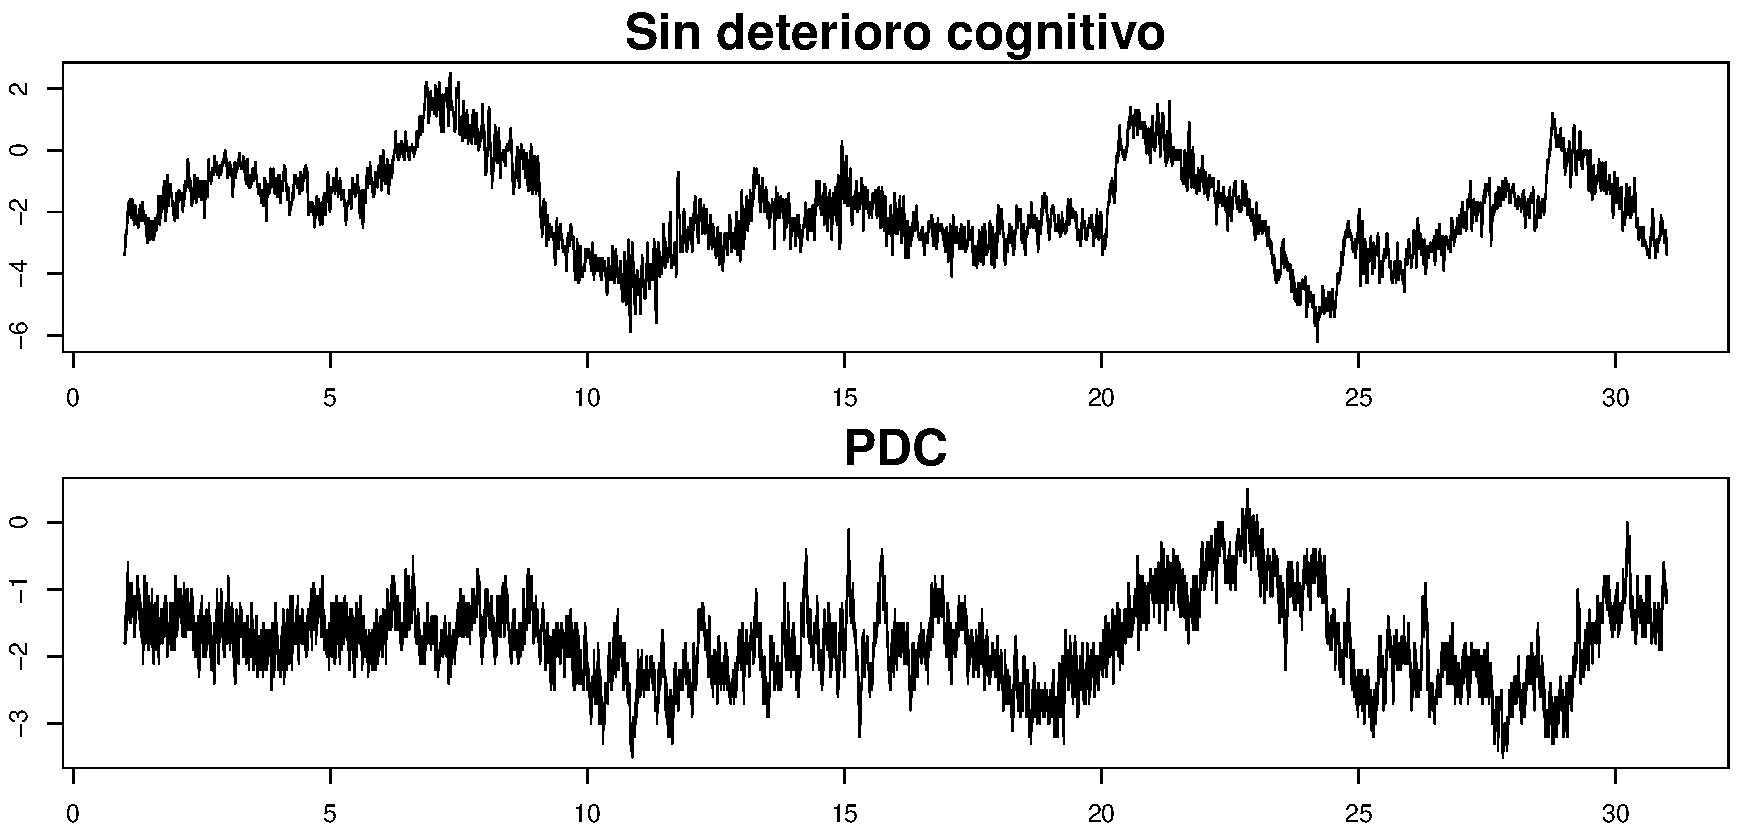
\includegraphics[width=.8\linewidth]{graficaintro.pdf}
\end{figure}

Adaptado de V\'azquez-Tagle y colaboradores (2016)

%Visualmente, el sue\~no MOR se caracteriza por movimientos oculares r\'apidos, aton\'ia muscular y 
%una actividad electroencefalogr\'afica desincronizada \cite{RosalesLagarde09}.

%%%%%%%%%%%%%%%%%%%%%%%%%%%%%%%%%%%%%%%%%%%%%%%%%%%%%%%%%%%%%%%%%%%%%%%%%%%%%%%%%%%%%%%%%%%%%%%%%%%
%%%%%%%%%%%%%%%%%%%%%%%%%%%%%%%%%%%%%%%%%%%%%%%%%%%%%%%%%%%%%%%%%%%%%%%%%%%%%%%%%%%%%%%%%%%%%%%%%%%

%%%%%%%%%%%%%%%%%%%%%%%%%%%%%%%%%%%%%%%%%%%%%%%%%%%%%%%%%%%%%%%%%%%%%%%%%%%%%%%%%%%%%%%%%%%%%%%%%%%
\chapter{Planteamiento del problema}

%Dentro de la teor\'ia de los ciclos de vida, la \'ultima etapa se refiere a la poblaci\'on 
%envejecida, en quienes lo caracter\'istico son las p\'erdidas f\'isicas, mentales, sociales y 
%econ\'omicas asociadas a la edad avanzada, con una vuelta a la dependencia sobre el grupo 
%intermedio. 
%En la caracterizaci\'on del grupo envejecido el deterioro de la salud es 
%un elemento principal. 
%El mayor impacto social y probablemente económico del envejecimiento, se desprende de los cambios en el estado de salud que conlleva.



%Tanto el deterioro cognitivo como las alteraciones del sueño son frecuentes en las personas de 
%edad avanzada y, aunque interfieren con la calidad de vida del individuo, no suelen ser 
%consideradas como patológicas sino como problemas asociados al propio envejecimiento.
%
%En un segundo momento, se pretenden medir aspectos cerebrales en el momento del sueño por medio 
%de un encefalograma para que con los resultados obtenidos de ambas fases y se determine la 
%diferencia entre los grupos de adulto mayor en evaluación cognitiva y su encefalografía.
%

%Visualmente, el sue\~no MOR se caracteriza por movimientos oculares r\'apidos, aton\'ia muscular y 
%una actividad electroencefalogr\'afica desincronizada \cite{RosalesLagarde09}.

%%%%%%%%%%%%%%%%%%%%%%%%%%%%%%%%%%%%%%%%%%%%%%%%%%%%%%%%%%%%%%%%%%%%%%%%%%%%%%%%%%%%%%%%%%%%%%%%%%%

\section{Justificaci\'on}

El deterioro cognitivo, que se define como ''un estado de transici\'on entre el envejecimiento 
normal y la demencia'' {Garrido09} es uno de los problemas de salud m\'as importantes en los 
pa\'ises desarrollados y sub-desarrollados que afecta directamente la calidad de vida de los 
adultos mayores lo que genera una mayor demanda de servicios de salud en el pa\'is.
Por otro lado, todav\'ia son incipientes las investigaciones para identificar 
factores de riesgo modificables de la demencia.
\cite{PlanAlzheimer04}

%Dada su relación con la edad, en la última década se ha dado un continuo incremento tanto en su incidencia como en su prevalencia, secundariamente al aumento progresivo de la longevidad en la población en general.

El estado de salud de la poblaci\'on de edad avanzada en su conjunto, tiene un peso espec\'ifico 
que recae en el sistema de salud en mayor o menor grado en funci\'on de la eficiencia de \'este. 
Por ello, existe la necesidad de que en el sistema de salud, realice una valoración integral del 
adulto mayor por parte del equipo de salud, para la detecci\'on temprana del deterioro cognitivo ya 
que  
%de nuestra población adulta mayor vive con algún tipo de deterioro, y 
al no ser diagnosticado adecuadamente incrementa el riesgo de evolucionar a demencia y por 
consiguiente largos y pesados periodos de cuidado y una atenci\'on especializada para recibir el 
tratamiento m\'as apropiado al que no todos tienen acceso, por los gastos que representa en todos 
los niveles. 
%Por otro lado, existe una gran demanda de datos fiables sobre la salud mental de los adultos mayores del estado de Hidalgo, dadas las limitaciones de los estudios epidemiológicos realizados hasta la fecha y los problemas metodológicos derivados de trabajar con diferentes localidades.

%Dada la relación entre el deterioro cognitivo y la calidad de sueño en adultos mayores, parece necesario reflexionar sobre las prevalencias del deterioro cognitivo, el rumbo que han tomado y su evaluación psicológica, las funciones mentales evaluadas, las metodologías y los resultados en México con énfasis particular en su relación con salud mental, así como considerar alternativas para valorar la función mental a nivel estatal y nacional con el apoyo de métodos de análisis biológicos. 

%%%%%%%%%%%%%%%%%%%%%%%%%%%%%%%%%%%%%%%%%%%%%%%%%%%%%%%%%%%%%%%%%%%%%%%%%%%%%%%%%%%%%%%%%%%%%%%%%%%

\section{Pregunta de investigaci\'on}

Considerando los registros de PSG como series de tiempo,
¿es plausible usar sus propiedades estad\'isticas dependientes del tiempo, espec\'ificamente
la estacionariedad d\'ebil,
como marcadores para el diagn\'ostico cl\'inico del DC --en alguna de 
sus fases-- en adultos mayores?

%%%%%%%%%%%%%%%%%%%%%%%%%%%%%%%%%%%%%%%%%%%%%%%%%%%%%%%%%%%%%%%%%%%%%%%%%%%%%%%%%%%%%%%%%%%%%%%%%%%

\section{Hip\'otesis}

Existen diferencias cuantificables estad\'isticamente significativas entre las propiedades
estad\'isticas dependientes del tiempo, de los registros de PSG
durante etapas espec\'ificas de sue\~no, en adultos
mayores con DC respecto a individuos control.

%%%%%%%%%%%%%%%%%%%%%%%%%%%%%%%%%%%%%%%%%%%%%%%%%%%%%%%%%%%%%%%%%%%%%%%%%%%%%%%%%%%%%%%%%%%%%%%%%%%

\section{Objetivo general}

A modo de estudio de casos retrospectivo,
deducir a partir de pruebas estad\'isticas formales (en el sentido matem\'atico) las propiedades
estad\'isticas de registros de PSG en adultos mayores con DC.

%%%%%%%%%%%%%%%%%%%%%%%%%%%%%%%%%%%%%%%%%%%%%%%%%%%%%%%%%%%%%%%%%%%%%%%%%%%%%%%%%%%%%%%%%%%%%%%%%%%

\subsection{Objetivos espec\'ificos}

\begin{itemize}
\item Investigar las definiciones de estacionariedad y sus consecuencias te\'oricas

\item Investigar en la literatura c\'omo detectar si es plausible que una serie de tiempo 
dada sea una realizaci\'on de un proceso d\'ebilmente estacionario, 
y bajo qu\'e supuestos es v\'alida esta caracterizaci\'on

\item Usando los an\'alisis hallados en la literatura para determinar si las series de tiempo,
obtenidas a partir de los registros PSG considerados, provienen de procesos
debilmente estacionarios.
Revisar si la informaci\'on obtenida en los diferentes sujetos muestra diferencias entre
sujetos con y sin DC

\item Determinar, para el caso de estudio presente, la validez de los \textbf{supuestos de 
estacionariedad d\'ebil}: su presencia o ausencia, en intervalos cortos o arbitrarios de tiempo
\end{itemize}

%%%%%%%%%%%%%%%%%%%%%%%%%%%%%%%%%%%%%%%%%%%%%%%%%%%%%%%%%%%%%%%%%%%%%%%%%%%%%%%%%%%%%%%%%%%%%%%%%%%

%%%%%%%%%%%%%%%%%%%%%%%%%%%%%%%%%%%%%

%%%%%%%%%%%%%%%%%%%%%%%%%%%%%%%%%%%%%%%%%%%%%%%%%%%%%%%%%%%%%%%%%%%%%%%%%%%%%%%%%%%%%%%%%%%%%%%%%%%
%%%%%%%%%%%%%%%%%%%%%%%%%%%%%%%%%%%%%%%%%%%%%%%%%%%%%%%%%%%%%%%%%%%%%%%%%%%%%%%%%%%%%%%%%%%%%%%%%%%
\section{Conceptos, fisiolog\'ia}

En esta secci\'on se exponen conceptos propios de la biolog\'ia y que ayudar\'an a definir
al sujeto de estudio: registros de PSG en adultos mayores con y sin PDC.
Se pretende que la exposici\'on sea accesible a\'un sin una preparaci\'on 
especializada en fisiolog\'ia, especialmente considerando que el autor pertenece a tal grupo.

%%%%%%%%%%%%%%%%%%%%%%%%%%%%%%%%%%%%%%%%%%%%%%%%%%%%%%%%%%%%%%%%%%%%%%%%%%%%%%%%%%%%%%%%%%%%%%%%%%%

\subsection{Adulto mayor}

Se define como adulto mayor a un individuo de 60 a\~nos o m\'as que habite un pa\'is en v\'ias de
desarrollo, o 65 a\~nos en pa\'ises desarrollados \cite{Hita14}.
En esta etapa 
%ocurren cambios fisiol\'ogicos, psicol\'ogicos y sociales
el organismo sufre cambios fisiolo\'ogicos y psicol\'ogicos que dificultan la capacidad de
adaptaci\'on al ambiente, teniendo como consecuencia una mayor suceptibilidad a padecer enfermedades
y morir en consecuencia \cite{Hita14}.


%El envejecimiento es un proceso biológico que se caracteriza por la disminución de las funciones 
%que hacen más susceptible al ser humano de padecer enfermedades y morir a consecuencia de 
%ellas [1]. 
%Durante esta etapa ocurren cambios biol\'ogicos, psicol\'ogicos y sociales, normales e 
%inherentes a todo individuo debido a que el organismo va perdiendo la habilidad para responder 
%ante el estr\'es y mantener la regulación homeost\'atica y metabólica, teniendo como consecuencia 
%la disminuci\'on de las capacidades cognitivas y de sobrevivencia, reflejándose en la imposibilidad 
%de adaptarse a situaciones de restricci\'on o sobrecarga de cualquier tipo [4,9,10]

El envejecimiento considerado normal viene determinado por una serie de procesos moleculares, 
celulares, fisiol\'ogicos y psicol\'ogicos que conducen directamente al deterioro de funciones 
cognitivas, específicamente en la atenci\'on y memoria \cite{Navarrete03,Park09}.
%Aunque el envejecimiento es un proceso normal, la 
La
funcionalidad durante la vejez no es homog\'enea
en general; se relaciona con el estilo de vida, los factores de riesgo, el acceso a la
educaci\'on y las acciones de promoci\'on a la salud realizadas en edades m\'as tempranas
\cite{Ohayon04,Sanhueza14}.

%A pesar de ser un proceso natural, no todos los individuos envejecen de la misma forma debido a 
%que la calidad de vida y funcionalidad durante la vejez est\'a relacionada con los aprendizajes 
%adquiridos durante la infancia, adolescencia y edad adulta \cite{Ohayon04}. 
%Los estilos de vida, los factores de riesgo, la accesibilidad a la educaci\'on y la promoci\'on 
%de la salud adoptados a lo largo de la vida son fundamentales al momento de llegar a esta etapa 
%para que en el presente de esta se logre autonom\'ia, a pesar de la edad y los padecimientos que 
%se tengan \cite{Sanhueza14}.

%%%%%%%%%%%%%%%%%%%%%%%%%%%%%%%%%%%%%%%%%%%%%%%%%%%%%%%%%%%%%%%%%%%%%%%%%%%%%%%%%%%%%%%%%%%%%%%%%%%

%\subsubsection{Cambios en la anatom\'ia cerebral con la vejez}

En un principio se consideraba que el envejecimiento cerebral ocurr\'ia fundamentalmente por una 
muerte neuronal programada \cite{Coleman87}, sin embargo, estudios realizados con tejido cerebral 
post mortem de adultos mayores que en vida fueron sanos, mostraron que dicha muerte neuronal no 
alcanza un 10\% en su totalidad \cite{Esiri07}. 
En este sentido, los cambios morfol\'gicos que 
sufren las neuronas durante el envejecimiento son abundantes, observ\'andose una importante 
disminuci\'on de la arborizaci\'n dendr\'itica as\'i como en la densidad y volumen \cite{Hita14}. 
%La disminución en la arborización dendr\'itica y de las espinas dendr\'iticas de las neuronas 
%piramidales de la corteza prefrontal, temporal superior, pre central y occipital \cite{Hita14}. 
%Dichas alteraciones morfol\'ogicas conducen durante el envejecimiento a una disminuci\'on de 
%la densidad sin\'aptica y a una desmielinizaci\'on ax\'onica en neuronas de la 
%neocorteza \cite{Terry}.
Con el paso del tiempo, la organizaci\'on an\'atomo-funcional del cerebro sufre modificaciones 
que traen como consecuencia la afectaci\'on de diferentes capacidades cognitivas, 
sin embargo, 
la vulnerabilidad de los circuitos neuronales ante los procesos que ocurren durante el 
envejecimiento no suceden de forma homog\'enea en todo el cerebro \cite{Hita14}.

%Por otro lado, la relevancia del estudio de los cambios anat\'omicos asociados al envejecimiento 
%fisiol\'ogico ha ido aumentando al permitir evaluar como dichos cambios se correlacionan con 
%el deterioro funcional y cognitivo que caracteriza a las personas mayores, facilita la 
%identificaci\'on de estadios tempranos de diferentes patolog\'ias neurodegenerativas estableciendo 
%diferencias entre estas y los cambios asociados al envejecimiento fisiol\'ogico \cite{Hita14}.

%%%%%%%%%%%%%%%%%%%%%%%%%%%%%%%%%%%%%%%%%%%%%%%%%%%%%%%%%%%%%%%%%%%%%%%%%%%%%%%%%%%%%%%%%%%%%%%%%%%

\subsection{El sue\~no}

%(Esta secci\'on tambi\'en es copiada, por el momento)

El sue\~no se define como ''un proceso vital c\'iclico complejo y activo, compuesto por varias 
fases y que posee una estructura interna caracter\'istica, con diversas interrelaciones en los 
sistemas hormonales y nerviosos'' \cite{FernandezConde07}. 
%Una suspensi\'on f\'acilmente reversible 
%de la interacci\'on sensoriomotriz con el medio ambiente, por lo general asociados con el 
%dec\'ubito y la inmovilidad.
El sue\~no en el ser humano se puede caracterizar por las siguientes propiedades\cite{CarrilloMora}
%Las caracter\'isticas conductuales que se asocian con el sue\~no en el ser humano pueden 
%enumerarse de la siguiente forma\cite{CarrilloMora} 
\begin{enumerate}
\item Disminuci\'on de conciencia y reactividad a est\'imulos externos
\item F\'acilmente reversible\footnote{Lo cual lo diferencia de otros estados 
patol\'ogicos como el estupor y el coma}
\item Inmovilidad y relajaci\'on muscular
\item Periodicidad t\'ipica circadiana (diaria)
\item Los individuos adquieren una postura estereotipada
\item La privaci\'on induce alteraciones conductuales y 
fisiol\'ogicas, adem\'as de que genera una ''deuda'' acumulativa
\end{enumerate}

%%%%%%%%%%%%%%%%%%%%%%%%%%%%%%%%%%%%%%%%%%%%%%%%%%%%%%%%%%%%%%%%%%%%%%%%%%%%%%%%%%%%%%%%%%%%%%%%%%%

%El sustrato neurol\'ogico relacionado con la ritmicidad del sueño se encuentra en el hipot\'alamo, 
%estructura que tiene diversidad de conexiones en el Sistema Nervioso Central, con el fin de 
%ejercer una funci\'on o funciones capaces de sincronizar el organismo 
%\cite{FernandezConde07,Cabrera14}.
%Las estructuras l\'imbicas, tales como la am\'igdala y el hipot\'alamo, tambi\'en estar\'ian 
%activadas, lo que explicar\'ia los fen\'omenos emotivos durante la fase de sue\~no REM ya que 
%las emociones est\'an directamente vinculadas con estas zonas cerebrales \cite{Bonet08}.

%%%%%%%%%%%%%%%%%%%%%%%%%%%%%%%%%%%%%%%%%%%%%%%%%%%%%%%%%%%%%%%%%%%%%%%%%%%%%%%%%%%%%%%%%%%%%%%%%%%
%%%%%%%%%%%%%%%%%%%%%%%%%%%%%%%%%%%%%%%%%%%%%%%%%%%%%%%%%%%%%%%%%%%%%%%%%%%%%%%%%%%%%%%%%%%%%%%%%%%

\subsection{Electroencefalograma}

%Esta secci\'on est\'a fuermente basada\footnote{A este punto, ya
%no es una copia, pero quiz\'a ser\'ia mejor diversificar las fuentes} 
%en el cap\'itulo de libro 
%''The origin of biopotentials'' de John William Clark \cite{clark98}.

La actividad el\'ectrica en el cerebro de animales ya hab\'ia sido descrita desde finales del
siglo XIX, pero se le atribuye al psiquiatra alem\'an Hans Berger ser el primero en analizar
este fen\'omeno sistem\'aticamente adem\'as de acu\~nar el t\'ermino ''electroencefalograma'' (EEG)
para referirse a las fluctuaciones en los potenciales de acci\'on registradas en el cerebro.
De manera convencional, la actividad el\'ectrica del cerebro 
se registra en tres locaciones diferentes: en la corteza cerebral
expuesta (electrocorticograma, ECoG), a trav\'es de agujas incrustadas en el tejido nervioso
(registro profundo), o el cuero cabelludo (EEG).

%La actividad el\'ectrica en el cerebro de animales con y sin anestesia ya hab\'ia sido descrito
%cualitativamente desde el siglo XIX, pero el primero en analizarla sistem\'aticamente fue el
%psiquiatra alem\'an Hans Berger, quien introdujo el t\'ermino electroencefalograma (EEG) para
%denotar las fluctuaciones en los potenciales registrados en el cerebro. [tengo citas sobre ello]
%De manera convencional, la actividad el\'ectrica del cerebro se registra usando tres tipos de
%electrodos: 'scalp', cortical y electrodos de profundidad.
%Cuando los electrodos se colocan en la superficie expuesta del cerebro (cortex) el
%registro se llama electrocorticograma (ECoG). Tambi\'en se pueden usar electrodos de aguja
%aislada fina --de varios dise\~nos-- incrustados en el tejido nervioso del cerebro, en
%cuyo caso el registro se conoce como 'registro profundo'. Seg\'un se reporta, el da\~no al
%tejido cerebral es sorprendentemente peque\~no si se usan agujas con un tama\~no
%y dise\~no adecuados.

As\'i la actividad el\'ectrica cerebral se mida
en el cuero cabelludo, la corteza cerebral o las profundidades 
del mismo,
las fluctuaciones de potenciales registrados representan una superposici\'on
de potenciales de campo producidos por una amplia variedad de 
generadores de corriente dentro de un medio conductor volum\'etrico --es decir, los elementos
neuronales activos generan, cada cual, corrientes que son conducidas y disipada a 
trav\'es del espacio.
A su vez, estos generadores de campos el\'ectricos corresponden a agregados de elementos
neuronales con interconexiones complejas: dendritas, somas y axones.
%M\'as a\'un, la arquitectura del tejido cerebral no es uniforme
%espacialmente.
A ello hay que adicionar que la arquitectura cerebral es altamente no homog\'enea.

%%%%%%%%%%%%%%%%%%%%%%%%%%%%%%%%%%%%%%%%%%%%%%%%%%%%%%%%%%%%%%%%%%%%%%%%%%%%%%%%%%%%%%%%%%%%%%%%%%%

%\subsubsection{Potenciales bioel\'ectricos del cerebro}

%Los registros unipolares de potencial en la superficie cortical, relativos a un potencial de
%referencia remoto, pueden ser vistos como una medida del potencial de campo integrado sobre la
%frontera de un volumen conductor 'grande' que contiene un conjunto de fuentes de potenciales de 
%campo.

%Bajo condiciones normales los potenciales de campo producidos por axones, en 
%la corteza cerebral, aportan muy poco al potencial registrado;
%%al potencial de superficie integrado; 
%esto d
Debido a que los axones en la corteza cerebral tienen orientaciones muy diversas --con
%orientaciones muy diversas 
respecto a la superficie-- y a que disparan de manera as\'incrona, el aporte neto de estos campos
al potencial registrado es negligible bajo condiciones normales.
%En consecuencia, su influencia neta sobre el potencial de campo en la superficie es negligible.
Una excepci\'on, muy importante, ocurre en caso de una respuesta evocada por un est\'imulo
simult\'aneo (s\'incronizado) del del n\'ucleo 
tal\'amico o de las aferentes nerviosas.
%, que se proyecta en el cortex v\'ia axones corticotal\'amicos).
Estas respuestas sincronizadas suelen tener una amplitud relativamente alta, y
son referidas como 'potenciales evocados'.
%, y su amplitud es
%relativamente alta.

%%%%%%%%%%%%%%%%%%%%%%%%%%%%%%%%%%%%%%%%%%%%%%%%%%%%%%%%%%%%%%%%%%%%%%%%%%%%%%%%%%%%%%%%%%%%%%%%%%%

\subsubsection{EEG cl\'inico}

El sistema m\'as usado para la colocaci\'on de los electrodos en el EEG con fines cl\'inicos es el 
'International Federation 10--20 system' \cite{Jasper58,AASM07} mostrado en la figura \ref{img1020}. 
Este sistema usa varios
referentes anat\'omicos estandarizados para la ubicaci\'on de los electrodos.

La representaci\'on de los canales de EEG es referida como un \textbf{montaje}
En un montaje bipolar, cada canal mide la diferencia entre dos electrodos adyacentes.
En un monntaje referencial, cada canal mide la diferencia entre un electrodo y un electrodo
de referencia, usualmente la oreja.
\footnote{Existen otros tipos de montaje, como el promedio (promedio sobre electrodos adyacentes,
como los sistemas 5\% y 10\%) o el Laplaciano (parecido al promedio, pero usando un filtrado
basado en pesos relacionados con la distancia entre electrodos). S\'olo hablo del referencial
y diferencial porque uno se usa en el estudio y otro es importante hist\'oricamente.}
Aunque los mismos eventos el\'ectricos se registran en cada uno de los montajes,
aparecen en un diferente formato seg\'un el caso. Los potenciales cambiantes
son amplificados por amplificadores diferenciales acoplados de alta ganancia.
La se\~nal resultante es grabada y graficada.

\begin{figure}
\centering
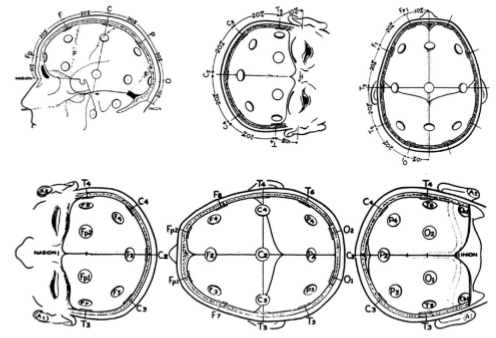
\includegraphics[width=0.8\linewidth]{figura_6.png} 
\caption{El sistema 10--20, recomendado por la
International Federation of EEG Societies. 
%\cite{Jasper58,AASM07}
}
\label{img1020}
\end{figure}

%The system most often used to place electrodes for monitoring the clinical
%EEG is the International Federation 10–20 system shown in Figure 4.28. This
%system uses certain anatomical landmarks to standardize placement of EEG
%electrodes. The representation of the EEG channels is referred to as a
%montage. 
%In the bipolar montage, each channel measures the difference
%between two adjacent electrodes. 
%In the referential montage, each channel
%measures the diffference between one electrode and a reference electrode,
%such as on the ear. In the average reference montage, each channel measures
%the difference between one electrode and the average of all other electrodes.
%In the Laplacian montage, each channel measures the difference between one
%electrode and a weighted average of the surrounding electrodes. The differ-
%ential amplifier requires a separate ground electrode plus differential inputs to
%the electrode connections. The advantage of using a differential recording
%between closely spaced electrodes (between successive pairs in the standard
%system, for example) is cancellation of far-field activity common to both
%electrodes; one thereby obtains sharp localization of the response. 
%Although
%the same electric events are recorded in each of the ways, they appear in a
%different format in each case. The potential changes that occur are amplified by
%high-gain, differential, capacitively coupled amplifiers. The output signals are
%recorded and displayed.

En el EEG cl\'inico de rutina, los electrodos son un problema: deben ser peque\~nos, deben estar
fijados al 'scalp' de manera sencilla con una distorsi\'on m\'inima debido al cuero cabelludo,
deben ser c\'omodos, y deben permanecer en el mismo sitio por largos periodos de tiempo.
El [encargado del registro] prepara la superficie del 'scalp' desengrasando el \'area de registro
limpi\'andola con alcohol, aplica una pasta conductora, pega los electrodos no-polarizables (Ag/AgCl)
al scalp con pegamento (coloid\'on), y los sostiene en el sitio con cintas de caucho
--o se usa una gorra de caucho que contiene todos los electrodos.

%In the routine recording of clinical EEGs, the input electrodes are a
%problem. They must be small, they must be easily affixed to the scalp with
%minimal disturbance of the hair, they must cause no discomfort, and they must
%remain in place for extended periods of time. Technicians prepare the surface
%of the scalp, degrease the recording area by cleaning it with alcohol, apply a
%conducting paste, and glue nonpolarizable Ag/AgCl electrodes to the scalp
%with a glue (collodion) and hold them in place with rubber straps, or use a
%rubber cap that contains all electrodes.

El EEG usualmente se registra con el sujeto despierto pero relajado, descansando en una cama con 
los ojos cerrados; la posici\'on debe ser tal que los artefactos debidos al movimiento de 
electrodos en el 'scalp' sean m\'inimas. 
La actividad muscular, de la cara, cuello, orejas, etc., es quiz\'a la forma m\'as sutil de 
contaminaci\'on de los registros de EEG cuando se busca actividad espont\'anea del cerebro
durante una actividad, o la actividad evocada por est\'imulos sensoriales.
Por ejemplo, el espectro de frecuencias del potencial de campo producido por m\'usculos faciales
medianamente contra\'idos, incluye componentes de frecuencia que bien cuadran en el rango
usual del EEG (0.5--100 Hz).
Una vez se ha conseguido el estado de reposo en un adulto normal, sus registros de scalp
muestran un ritmo alfa dominante en el \'area parietal-occipital, mientras que en \'area
frontal ha un ritmo beta con baja amplitud y alta frecuencia --adem\'as del ritmo alfa.
En un sujeto normal hay cierta simetr\'ia entre los registros de los hemisferios derecho e 
izquierdo. 
La variedad de artefactos conocidos es muy basta.

%The EEG is usually recorded with the subject awake but resting recumbent
%on a bed with eyes closed. With the patient relaxed in such a manner, artifacts
%from electrode-lead movement are significantly reduced, as are contaminating
%signals from the scalp. 
%Muscle activity from the face, neck, ears, and so on is
%perhaps the most subtle contaminant of EEG records in the recording of both
%spontaneous ongoing activity in the brain and activity evoked by a sensory
%stimulus (evoked response). 
%For example, the frequency spectrum of the field
%produced by mildly contracted facial muscles contains frequency components
%well within the nominal EEG range (0.5 to 100 Hz). After technicians have
%achieved resting, quiescent conditions in the normal adult subject, the subject’s
%scalp recordings show a dominant alpha rhythm in the parietal-occipital areas,
%whereas in the frontal areas, there is a low-amplitude, higher-frequency beta
%rhythm in addition to the alpha rhythm. In the normal subject there is
%symmetry between the recordings of the right and left hemispheres. There
%can be a wide range of EEG measurement artifacts.

En general hay una relaci\'on entre el grado de actividad cerebral
y la 'frecuencia promedio' del EEG: la frecuancia incrementa progresivamente cuando hay altos
grados de actividad. Por ejemplo, las ondas delta se encuentran frecuentemente durante el
estupor, anestesia quir\'urgica, y sue\~no; las ondas theta son comunes en infantes;
las ondas alfa ocurren en estado de relajaci\'on; las ondas beta aparecen durante actividad
mental intensa.
Sin embargo, durante periodos de actividad mental las ondas se vuelven m\'as as\'incronas
que sincronizadas, de modo que la magnitud del potencial integrado de superficie
decrece a pesar de la alta actividad cortical.

%In general there is a relationship between the degree of cerebral activity
%and the average frequency of the EEG rhythm: The frequency increases
%progressively with higher and higher degrees of activity. For example, delta
%waves are frequently found in stupor, surgical anesthesia, and sleep; theta
%waves in infants; alpha waves during relaxed states; and beta waves during
%intense mental activity. However, during periods of mental activity, the waves
%usually become asynchronous rather than synchronous, so that the magnitude
%of the summed surface potential recording decreases despite increased cortical
%activity.

%%%%%%%%%%%%%%%%%%%%%%%%%%%%%%%%%%%%%%%%%%%%%%%%%%%%%%%%%%%%%%%%%%%%%%%%%%%%%%%%%%%%%%%%%%%%%%%%%%%

\subsection{Ritmos de sue\~no en el EEG}

Los registros de EEG desde el cuero cabelludo muestran una actividad el\'ectrica oscilatoria 
continua y cambiante. Tanto la intensidad como los patrones de esta actividad est\'an determinados
por los eventos de excitaci\'on conjunta del cerebro, resultante de las funciones en el
sistema reticular de activaci\'on del tallo cerebral \cite{Clark98}.
Estas 'ondas' observadas en los registros de potenciales el\'ectricos en el cerebro 
(\ref{ritmos}) son referidas como
\textbf{ondas cerebrales}, mientras que %el registro \textit{per se} recibe el nombre de EEG.

La frecuencia de las ondas cerebrales var\'ia entre 0.5 y 100 Hz, 
se ha identificado que su composici\'on est\'a fuertemente
relacionada con el grado de actividad cerebral, habiendo --por ejemplo-- diferencias claras
entre registros durante vigilia y sue\~no.
Aunque la mayor parte del tiempo el EEG es irregul y no muestra patrones claros,
es relativamente com\'un que muestre ondas cerebrales relativamente organizadas; para su estudio,
estas se clasifican en cuatro grandes grupos: alfa, beta, gamma, delta.


\begin{figure}
\centering
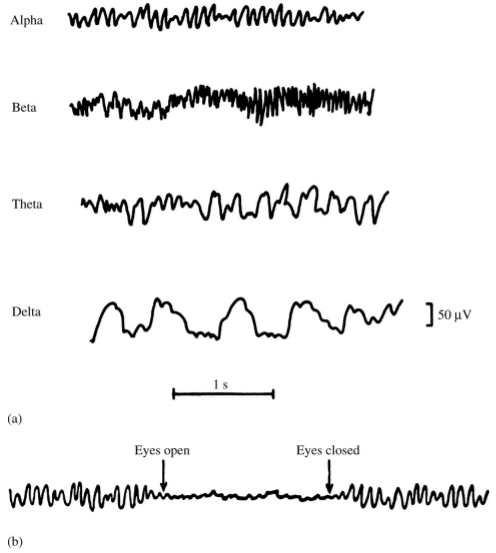
\includegraphics[width=0.7\linewidth]{figura_4.png} 
\caption{\textbf{(a)} Diferentes tipos de ondas normales en el EEG.
\textbf{(b)} Supresi\'on del ritmo alfa debido a una descarga dessincronizada cuando
el paciente abre los ojos.
%(From A. C. Guyton, Structure and Function of the Nervous System, 2nd ed.,
%Philadelphia: W.B. Saunders, 1972; used with permission.)
[Estos gr\'aficos ser\'an reconstruidos]
}
\label{ritmos}
\end{figure}


Las ondas alfa ocurren en frecuencias entre 8 y 13 Hz. 
Se encuentran en
los EEG --bajo condiciones normales--
de sujetos despiertos en un estado de quietud del pensamiento.
Estas ondas ocurren m\'as intensamente en la regi\'on occipital, pero tambi\'en pueden ser
registradas en las regiones frontal y parietal. Su voltaje aproximado est\'a entre 20 y 200 mV.
Cuando el sujeto duerme, las ondas alfa desaparecen completamente. 
Cuando el sujeto est\'a
despierto y su atenci\'on se dirige a una actividad mental espec\'ifica, las ondas alfa
son reemplaxadas por ondas dessincronizadas de mayor frecuencia y menor voltaje.
%En la figura \ref{ritmos} se muestra este efecto con la acci\'on de cerrar los ojos.

Las ondas beta ocurren en el rango de frecuencias de 14 a 30 Hz.
%, y usualmente
%--en especial durante actividad mental intensa-- hasta 50 Hz.
Normalmente se registran en las regiones parietal y frontal. A veces se les divide
 en dos tipos: beta I y beta II. Las ondas beta I tienen una frecuencia de cerca del doble a
 las ondas alfa, y son afectadas de manera similar por la actividad mental --desaparecen
y son reemplazadas por ondas dessincronizadas de menor amplitud.
Las ondas beta II, en cambio, aparecen durante una activaci\'on intensa del sistema nervioso
central y durante tensi\'on.

%Beta waves normally occur in the frequency range of 14 to 30 Hz, and
%sometimes—particularly during intense mental activity—as high as 50 Hz.
%These are most frequently recorded from the parietal and frontal regions of the
%scalp. They can be divided into two major types: beta I and beta II. The beta I
%waves have a frequency about twice that of the alpha waves. They are affected
%by mental activity in much the same way as the alpha waves (they disappear
%and in their place appears an asynchronous, low-voltage wave). The beta II
%waves, on the other hand, appear during intense activation of the central
%nervous system and during tension. Thus one type of beta activity is elicited by
%mental activity, whereas the other is inhibited by it.

Las ondas theta tienen frecuencias entre 4 y 7 Hz. Ocurren principalmente en las regiones
parietal y temporal en ni\~nos, pero pueden aparecer en algunos adultos durante 
estr\'es emocional, sobre todo durante periodos de decepsi\'on y frustraci\'on.
%Por ejemplo, pueden ser inducidos en el EEG de una persona frustrada una vez se le permite
%disfrutar una experiencia placentera, la cual es removida s\'ubitamente. Esto causa
%aproximadamente 20 s de ondas theta.

%Theta waves have frequencies between 4 and 7 Hz. These occur mainly in
%the parietal and temporal regions in children, but they also occur during
%emotional stress in some adults, particularly during periods of disappointment
%and frustration. For example, they can often be brought about in the EEG of a
%frustrated person by allowing the person to enjoy some pleasant experience
%and then suddenly removing the element of pleasure. This causes approxi-
%mately 20 s of theta waves.

Las ondas delta incluyen todas las ondas del EEG 'abajo de' 3.5 Hz. 
%A veces, estas ondas s\'olo
%aparecen cada 2 o 3 seg. 
Ocurren generalmente en el sue\~no profundo en infantes,
y despu\'es de enfermedades org\'anicas serias del cerebro.
Tambi\'en pueden ser registradas en cerebros de animales a los cuales se ha hecho 
transsecci\'on subcortical, produciendo una separaci\'on funcional entre la corteza
cerebral y el 
sistema reticular de activaci\'on del tallo cerebral. 
%Entonces, las ondas delta s\'olo pueden ocurrir en la cortreza cerebral,
%independientemente de la actividad en las regiones m\'as bajas del cerebro.

%%%%%%%%%%%%%%%%%%%%%%%%%%%%%%%%%%%%%%%%%%%%%%%%%%%%%%%%%%%%%%%%%%%%%%%%%%%%%%%%%%%%%%%%%%%%%%%%%%%

%\subsection{Patrones en el sue\~no}

%When an individual in a relaxed, inattentive state becomes drowsy and falls
%asleep, the alpha rhythm is replaced by slower, larger waves 
%(\ref{ritmosEEG},\cite{Jasper42}). 

En el sue\~no profundo se observan ondas delta muy irregulares. Junto con ellas, durante el sue\~no
medianamente profundo, ocurren trenes cortos de ondas parecidas a las alfa y que son referidas como
\textit{husos de sue\~no} (sleep spindles). El ritmo alfa y los husos de sue\~no 
est\'a sincronizados en
el sue\~no y la somnolencia, en contraste con la actividad irregular, desincronizada y de bajo 
voltaje registrada en estado de alerta.

%In
%deep sleep, very large, somewhat irregular delta waves are observed. Inter-
%spersed with these waves—during moderately deep sleep—are bursts of alpha-
%like activity called sleep spindles. The alpha rhythm and the patterns of the
%drowsy and sleeping subject are synchronized, in contrast with the low-voltage
%desynchronized, irregular activity seen in the subject who is in an alert state.
%The high-amplitude, slow waves seen in the EEG of a subject who is asleep
%are sometimes replaced by rapid, low-voltage irregular activity resembling that
%obtained in alert subjects. 
%However, the sleep of a subject with this irregular
%pattern is not interrupted; in fact, the threshold for arousal by sensory stimuli is
%elevated. 
%This condition has therefore come to be called paradoxical sleep.
%During paradoxical sleep, the subject exhibits rapid, roving eye movements.

A veces,
las ondas lentas de amplitud alta son reemplazadas durante el sue\~no por ondas r\'apidas de
bajo voltaje, irregulares, que recuerdan la actividad en el EEG durante el estado de alerta.
La presencia de estos patrones irregulares no interrumpen el sue\~no, sino que 
incluso se incrementa el umbral
para que los est\'imulos externos despierten al paciente; 
este comportamiento es referido como ''sue\~no parad\'ogico''.
Durante este sue\~no parad\'ogico, el sujeto exhibe movimientos oculares r\'apidos,
raz\'on por la cual se le conoce como ''sue\~no de movimientos oculares r\'apidos'' (MOR).
%o sue\~no parad\'ojico debido a que se presentan simult\'aneamente
%una reducci\'on marcada en el tono
%muscular y los movimientos oculares r\'apidos.
%La etapa del sue\~no donde se encuentran los husos de sue\~no y la actividad
%sincronizada 
La etapa fuera del sue\~no
es referida como sue\~no no-MOR (NMOR) o sue\~no de ondas lentas.
Los sujetos humanos que despiertan durante la fase de sue\~no MOR suelen reportar que
ten\'ian enso\~naciones, a diferencia de aquellos que despiertan durante la fase NREM.

%For this reason, it is also called rapid-eye-movement sleep, or REM sleep.
%Conversely, spindle or synchronized sleep is frequently called nonrapid-eye-
%movement (NREM), or slow-wave sleep. Human subjects aroused at a time
%when their EEG exhibits a paradoxical (REM) sleep pattern generally report
%that they were dreaming, whereas individuals wakened from spindle sleep do
%not. 

%Estas observaciones sugieren que el sue\~no MOR y las enso\~naciones est\'an fuermente
%asociadas. De manera parad\'ojica, durante el sue\~no REM hay una reducci\'on marcada en el tono
%muscular a pesar de los movimientos oculares r\'apidos.

%This observation and other evidence indicate that REM sleep and
%dreaming are closely associated. It is interesting that during REM sleep, there
%is a marked reduction in muscle tone, despite the rapid eye movements.

\begin{figure}
\centering
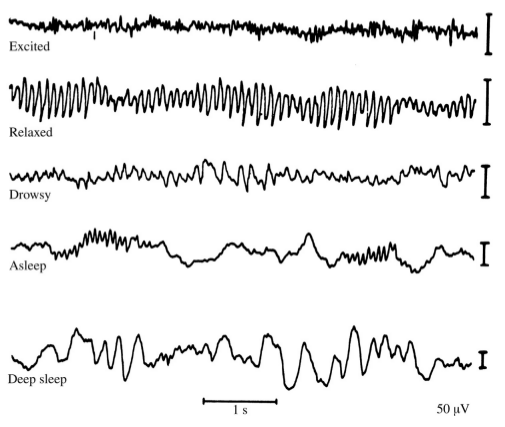
\includegraphics[width=0.7\linewidth]{figura_7.png} 
\caption{Los cambios en el EEG que ocurren durante el sue\~no en un sujeto.
Las marcas de calibraci\'on corresponden a 50 mV.
%H. Jasper, ‘‘Electrocephalography.’’ In Epilepsy and Cerebral Localization, W.
%G. Penfield and T. C. Erickson (eds.). Springfield, IL: Charles C. Thomas,
%1941.)
[Estos gr\'aficos ser\'an redibujados]
}
\label{ritmosEEG}
\end{figure}

%%%%%%%%%%%%%%%%%%%%%%%%%%%%%%%%%%%%%%%%%%%%%%%%%%%%%%%%%%%%%%%%%%%%%%%%%%%%%%%%%%%%%%%%%%%%%%%%%%%

\subsection{Etapas del sue\~no}

El sue\~no normal se divide en dos etapas: sue\~no  MOR (fase R)
%\footnote{Tambi\'en conocido como
%REM (Rapid-eyemovement)} (movimiento-ocular-r\'apido) 
y sue\~o no-MOR (fase N), los cuales se diferencian 
fundamentalmente por sus rasgos electroencefalogr\'aficos y una serie de caracter\'isticas 
fisiol\'ogicas --de los cuales surgen sus nombres.
Cabe mencionar que
la nomenclatura acerca de las fases del sue\~no ha sido 
recientemente modificada por la Academia Americana de Medicina del Sueño en 2007, 
de modo que en este trabajo se usar\'an ambas nomenclaturas siempre que sea posible, por fines
de compatibilidad con la terminolog\'ia usual.

%Una herramienta tecnol\'ogica que ha sido de vital importancia para el estudio de la fisiolog\'ia 
%del sue\~no es el electroencefalograma (EEG). De forma muy simplificada, el EEG es el la 
%representaci\'on gr\'afica y digital de las oscilaciones que muestra la actividad el\'ectrica 
%del cerebro, al ser registrada mediante electrodos colocados encima de la piel cabelluda en 
%distintas regiones de la cabeza \cite{Hita14}.

%El sue\~no MOR se caracteriza por la presencia de ondas de bajo voltaje y alta frecuencia en el 
%EEG, aton\'ia muscular y movimientos oculares r\'apidos, adem\'as es donde se presentan 
%la mayor\'ia de los sue\~nos. 
%El sue\~no no-MOR se compone de cuatro fases, 1 y 2, que son de sue\~no ligero, y 3 y 4 de 
%sue\~no profundo, las mismas que transcurren de manera secuencial desde la primera hasta la 
%cuarta fase, que es la fase reparadora del sue\~no, aquella que produce en la persona la 
%sensaci\'on de haber descansado cuando se levanta 13,22,43.

%Las características de las fases del sueño no-MOR incluyen cuatro etapas, la primera que 
%corresponde a la transición de la vigilia al sueño; la etapa 2 es la intermedia (mayor porcentaje 
%del tiempo de sueño) y en el EEG aparecen husos de sueño y los complejos K. La etapa 3 es la del 
%sueño relativamente profundo, representado en el electroencefalograma por ondas lentas de gran 
%amplitud, y la etapa 4o de sueño profundo con más del 50\% de ondas lentas de gran amplitud13.

%Durante el estado de alerta, mientras se mantienen los ojos cerrados, en el EEG se observan 
%oscilaciones de la actividad eléctrica que suelen encontrarse entre 8-13 ciclos por segundo (Hz), 
%principalmente a nivel de las regiones occipitales (ritmo alfa). Durante el sueño ocurren cambios 
%característicos de la actividad eléctrica cerebral que son la base para dividir el sueño en varias 
%fases. Como ya se mencionó, el sueño suele dividirse en dos grandes fases que, de forma normal, 
%ocurren siempre en la misma sucesión: todo episodio de sueño comienza con el llamado sueño sin 
%movimientos oculares rápidos (No MOR), que tiene varias fases, y después pasa al sueño con 
%movimientos oculares rápidos (MOR). 

%%%%%%%%%%%%%%%%%%%%%%%%%%%%%%%%%%%%%%%%%%%%%%%%%%%%%%%%%%%%%%%%%%%%%%%%%%%%%%%%%%%%%%%%%%%%%%%%%%%

\subsubsection{Sueño no-MOR (N)}

\begin{description}
\item[Fase 1 (N1)] Corresponde con la somnolencia o el inicio del sue\~no ligero, en ella es muy 
f\'acil despertarse. La actividad muscular disminuye paulatinamente y pueden observarse algunas 
breves sacudidas musculares s\'ubitas que a veces coinciden con una sensación de ca\'ida 
(mioclon\'ias h\'ipnicas). En el EEG se observa actividad de frecuencias mezcladas, pero de bajo 
voltaje y algunas ondas agudas (ondas agudas del v\'ertex). 

\item[Fase 2 (N2)] En el EEG se caracteriza por que aparecen patrones espec\'ificos de actividad 
cerebral llamados \textbf{husos de sue\~no} y \textbf{complejos K}. F\'isicamente la 
temperatura, la frecuencia cardiaca y respiratoria comienzan a disminuir paulatinamente. 

\item[Fases 3 y 4 (N3)] Sue\~no de ondas lentas, es la fase de sue\~no no-MOR m\'as profunda, 
y en el EEG se observa actividad de frecuencia muy lenta (< 2 Hz).
\end{description}

%%%%%%%%%%%%%%%%%%%%%%%%%%%%%%%%%%%%%%%%%%%%%%%%%%%%%%%%%%%%%%%%%%%%%%%%%%%%%%%%%%%%%%%%%%%%%%%%%%%

\subsubsection{Sueño MOR (R)}

Se caracteriza por la presencia de movimientos oculares r\'apidos. F\'isicamente el tono de todos 
los m\'usculos disminuye (con excepción de los m\'usculos respiratorios y los esf\'interes vesical 
y anal), as\'i mismo la frecuencia cardiaca y respiratoria se vuelve irregular.%,
%e incluso puede 
%incrementarse y 
%existe erección espontánea del pene o del clítoris. 
Durante el sue\~no MOR se producen la mayor\'ia de las enso\~naciones (lo que conocemos 
coloquialmente como sue\~nos), y la mayor\'ia de los pacientes que despiertan durante esta fase 
suelen recordar v\'ividamente el contenido de sus enso\~naciones \cite{Chokroverty09}.

%Por otro lado, las necesidades de sueño son muy variables según la edad y las circunstancias 
%individuales 43,54:
%Un niño recién nacido duerme casi todo el día, con una proporción próxima al 50\% del denominado 
%sueño «activo», que es el equivalente del sueño MOR. A lo largo de la lactancia los períodos de 
%vigilia son progresivamente más prolongados y se consolida el sueño de la noche; además, la 
%proporción de sueño MOR desciende al 25-30 \%, que se mantendrá durante toda la vida. Entre el 1er 
%y 3er año de vida el niño ya sólo duerme una o dos siestas. Entre los 4 y 5 años y la adolescencia 
%los niños son hipervigilantes, muy pocos duermen siesta, pero tienen un sueño nocturno de 9-10 
%horas bien estructurado en 5 ciclos o más. Por lo que se refiere a los individuos jóvenes, en 
%ellos reaparece en muchos casos la necesidad fisiológica de una siesta a mitad del día43,55.

%%%%%%%%%%%%%%%%%%%%%%%

%La necesidad de sue\~no en un adulto puede oscilar entre 5 y 9 horas. Asimismo, var\'ia 
%notablemente el horario de sueño entre noct\'ambulos y madrugadores. En \'epocas de mucha actividad 
%intelectual o de crecimiento o durante los meses del embarazo, puede aumentar la necesidad de 
%sue\~no, mientras que el estr\'es, la ansiedad o el ejercicio f\'isico practicado por la tarde 
%pueden reducir la cantidad de sue\~no. 

%%%%%%%%%%%%%%%%%%%%%%%

%Los estudios efectuados en individuos aislados de influencias exteriores han mostrado que la 
%tendencia fisiológica general es a retrasar ligeramente la fase de sueño con respecto al ciclo 
%convencional de 24 horas y a dormir una corta siesta “de mediodía” 43,56. 
Un adulto j\'oven pasa aproximadamente entre 70--100 min en el sue\~no no-MOR para despu\'es entrar 
al sue\~no MOR, el cual puede durar entre 5--30 min; este ciclo se repite cada hora y media.
%durante toda la noche de sue\~no. 
A lo largo de la noche pueden presentarse normalmente entre 4 y 6 ciclos de 
sue\~no MOR.
En los ancianos se va fragmentando el sue\~no nocturno con frecuentes episodios de despertar, y se 
reduce mucho el porcentaje de sue\~no en fase 4 y no tanto el de sue\~no MOR, que se mantiene 
m\'as constante.% a lo largo de la vida. 
%Las personas de edad avanzada tienen tendencia a aumentar el tiempo de permanencia en la cama. 
%Muchas de ellas dormitan 
Adicionalmente, muchos adultos mayores dormitan
%f\'acilmente 
durante el d\'ia varias siestas cortas\cite{CarrilloMora}.

%%%%%%%%%%%%%%%%%%%%%%%%%%%%%%%%%%%%%%%%%%%%%%%%%%%%%%%%%%%%%%%%%%%%%%%%%%%%%%%%%%%%%%%%%%%%%%%%%%%

%\subsection{Alteraciones del ciclo vigilia-sueño}
%
%La relevancia que tiene el sueño para para la supervivencia de un individuo es la cantidad de horas que este duerme a lo largo de su vida, mismas que depende fundamentalmente de sus necesidades fisiológicas y de las demandas del ambiente al que está expuesto 4,57
% En el caso de los humanos, es posible establecer una clasificación de patrones de sueño en función de su duración (corta, intermedia y larga) 4. Las personas que muestran un patrón de sueño intermedio, es decir, duración aproximada de entre 7-8 horas, presentan un mejor estado de salud a lo largo de su vida, comparado con los individuos de duración de sueño corta o excesivamente larga que frecuentemente tienen de problemas de salud y/o laborales 42,45,46 . 
 
%La estabilidad del sue\~no nocturno es otro factor a tener en cuenta debido a que es razonable 
%pensar que un sue\~no muy fragmentado no cumplir\'a con sus funciones fisiol\'ogicas de igual forma 
%que un patr\'on de sue\~no estable a lo largo de la noche.

%%%%%%%%%%%%%%%%
%%%%%%%%%%%%%%%%
%
%Los adultos mayores informan que duermen menos durante la noche, y se acuestan y se despiertan 
%m\'as temprano de lo habitual. Adem\'as, tardan m\'as tiempo en conciliar el sue\~no, se 
%despiertan con m\'as frecuencia durante la noche y la duraci\'on de estos despertares es 
%m\'as prolongada 58,59.
%
%%%%%%%%%%%%%%%%
%%%%%%%%%%%%%%%%

%La disminución del tiempo de sueño asociada a un incremento de la somnolencia diurna incide negativamente en la función cerebral del día siguiente 60
%Por otro lado, existen diversas formas de pérdida de sueño13,25,46: a) la privación de sueño, que quiere decir la suspensión total del sueño por un periodo ($>$ 24 h), b) la restricción del sueño, que significa una disminución del tiempo habitual de sueño, generalmente de forma crónica, y c) la fragmentación del sueño, que significa la interrupción repetida (despertares) de la continuidad del sueño14. Todos estos tipos de alteraciones del sueño han demostrado afectar distintas funciones cognitivas y variedades de memoria en mayor o menor grado.

%Las alteraciones de sueño específicamente en personas mayores se han asociado con la presencia de enfermedades crónicas, problemas físicos y de salud mental 3

%%%%%%%%%%%%%%%%%%%%%%%%%%%%%%%%%%%%%%%%%%%%%%%%%%%%%%%%%%%%%%%%%%%%%%%%%%%%%%%%%%%%%%%%%%%%%%%%%%%
%%%%%%%%%%%%%%%%%%%%%%%%%%%%%%%%%%%%%%%%%%%%%%%%%%%%%%%%%%%%%%%%%%%%%%%%%%%%%%%%%%%%%%%%%%%%%%%%%%%

%%%%%%%%%%%%%%%%%%%%%%%%%%%%%%%%%%%%%%%%%%%%%%%%%%%%%%%%%%%%%%%%%%%%%%%%%%%%%%%%%%%%%%%%%%%%%%%%%%%
%%%%%%%%%%%%%%%%%%%%%%%%%%%%%%%%%%%%%%%%%%%%%%%%%%%%%%%%%%%%%%%%%%%%%%%%%%%%%%%%%%%%%%%%%%%%%%%%%%%

\section{Conceptos, matem\'aticas}

En esta secci\'on se describen los conceptos b\'asicos de la teor\'ia espectral 'cl\'asica' para 
procesos estacionarios, y la generalizaci\'on hecha por Priestley para procesos no-estacionarios. 
De forma m\'as bien pragm\'atica, la descripci\'on est\'a
 fuertemente inspirada por el libro 'Spectral Analysis and Time Series' 
de M. B. Priestley \cite{Priestley81}, ya que este est\'a expl\'icitamente dirigido a un p\'ublico 
sin un trasfondo matem\'atico.

Se suponen conocidos varios temas b\'asicos de probabilidad y estad\'istica:
variables aleatorias, valores esperados y momentos, estimadores y sus propiedades.
Con el fin de presentar la notaci\'on usada, se incluyen algunos conceptos previos a la 
definici\'on per se de estacionariedad y estimadores en el dominio de frecuencias.
%Chatfield (The Analysis of Time Series: An Introduction, 2003)

%%%%%%%%%%%%%%%%%%%%%%%%%%%%%%%%%%%%%%%%%%%%%%%%%%%%%%%%%%%%%%%%%%%%%%%%%%%%%%%%%%%%%%%%%%%%%%%%%%%

\subsection{Estacionariedad d\'ebil}

Para hablar formalmente de procesos estoc\'asticos como modelos, antes 
conviene escribir su definici\'on desde el punto de vista matem\'atico. Las siguientes definiciones
son aplicables tanto para procesos en tiempo continuo
como para procesos a tiempo discreto; aunque el objeto de estudio, el EEG, se considera 
un fen\'omeno continuo, s\'olo es posible registrarlo durante un conjunto finito de puntos 
en el tiempo.

\begin{defn}[Proceso estoc\'astico]
Un proceso estoc\'astico $\{ X(t) \}$ es una familia de variables aleatorias 
en los reales,
indexadas por
$t \in T \subseteq \R$.
%, mientras que una observaci\'on
%de $\{X(t)\}$ ser\'a denotada por $(x_1,x_2,\dots)$
\end{defn}

Como notaci\'on, una realizaci\'on de $X(t)$ ser\'a denota por $x_t$. 
Las funciones de densidad de probabilidad y de probabilidad acumulada para $X(t)$ ser\'an
referidas, respectivamente, como $f_{X(t)}$ y $F_{X(t)}$
%Cabe destacar que en esta definici\'on se omiti\'o intencionalmente pedir que las variables
%aleatorias sea reales, ya que eventualmente se considerar\'an procesos en los complejos.
Cabe enfatizar que para cada valor de $t$,
%tiempo $t$, 
$X(t)$ es una variable aleatoria; no se presupone ninguna conexi\'on entre ellas.
%con su funci\'on de densidad de probabilidad,
%sus momentos [s\'olo se consideran va's con al menos segundos momentos finitos], etc.


La caracter\'istica principal 
investigada en este trabajo hace referencia a la ''estacionariedad''. De manera 
informal, esta propiedad se refiere a que las variables aleatorias que conforman un proceso
estoc\'astico sean b\'asicamente iguales --dicho con otras palabras, que las propiedades
del proceso sean invariantes en el tiempo. 
Una definici\'on que satisface fielmente est\'a descripci\'on es la de estacionariedad 
en el sentido fuerte o estricto.
El t\'ermino ''tiempos admisibles'' simplemente indica que la definici\'on es la misma para
procesos a tiempo discreto o continuo, bajo restricciones obvias.

\begin{defn}[Estacionariedad fuerte]
Un proceso estoc\'astico $\{ X(t) \}$ es fuertemente estacionario si, para cualquier 
conjunto de tiempos admisibles $t_1,t_2,\dots,t_n$ y cualquier $\tau$ tal que 
 $t_i+\tau$ son tiempos admisibles para $i = 1, 2, \dots n$;
se cumple que
\begin{equation*}
F_{\left(X(t_1),X(t_2),\dots,X(t_n)\right) }
\equiv
F_{\left(X(t_1+\tau),X(t_2+\tau),\dots,X(t_n+\tau)\right)}
\end{equation*}

Donde $F_{\left(X(t_1),X(t_2),\dots,X(t_n)\right) }$ es la funci\'on de distribuci\'on de
probabilidad conjunta del vector $\left(X(t_1),X(t_2),\dots,X(t_n)\right)$
\end{defn}

Esta definici\'on, sin embargo, no resulta muy \'util en el contexto de la estad\'istica:
si se supone que el registro de un fen\'omeno puede interpretarse como \textbf{una} 
realizaci\'on de
un proceso estoc\'astico, entonces para cada tiempo se tiene una \'unica observaci\'on
de cada variable aleatoria. A esto hay que a\~nadir que, para un fen\'omeno continuo,
no todas los tiempos son registrables.
Luego, si no existe la garant\'ia de que las propiedades de estas variables aletorias sean
''similares'', entonces es virtualmente imposible obtener mayor informaci\'on de ellas.

Es bajo estas limitaciones que se motiva un concepto de estacionariedad m\'as d\'ebil, pero que
satisfaga ''suficientes teoremas importantes'' y que sea relevante bajo las restricciones
propias de diferentes campos. En este trabajo se ha optado por la llamada 
''estacionariedad d\'ebil'' o estacionariedad de orden 2, que recibe su nombre como caso
particular de la ''estacionariedad de orden $m$''.

\begin{defn}[Estacionariedad de orden $m$]
Un proceso estoc\'astico $\{ X(t) \}$
se dice estacionario de orden $m$ si, para cualquier 
conjunto de tiempos admisibles $t_1,t_2,\dots,t_n$ y cualquier $\tau \in \R$
se cumple que
\begin{equation*}
\E{ X^{m_1}(t_1)X^{m_2}(t_2)\cdots X^{m_n}(t_n) }
=
\E{ X^{m_1}(t_1+\tau)X^{m_2}(t_2+\tau)\cdots X^{m_n}(t_n+\tau) }
\end{equation*}
Para cualesquiera enteros $m_1,m_2,\dots,m_n$ tales que $m_1+m_2+\dots+m_n \leq m$
\label{est_orden_m}
\end{defn}

La estacionariedad d\'ebil no pide que la funci\'on
de distribuci\'on conjunta tenga determinada forma, sino que los momentos conjuntos sean 
invariantes ante traslaciones en el tiempo. Para entender mejor esta diferencia, consid\'erense
tres procesos $\{X(t)\}$, $\{Y_1(t)\}$ y $\{Y_2(t)\}$, de modo que el primero es
estacionario en el sentido fuerte, el segundo es estacionario de orden 1 y el tercero es
estacionario de orden 2.
\begin{itemize}
\item Por definici\'on $F_{X(t) } \equiv F_{X(t+\tau)}$ para cualesquieras $t$, $t+\tau$
admisibles; entonces $\E{X(t)} = \mu_X$ es constante
\item Por definici\'on
para cualesquieras $t$, $t+\tau$ admisibles se tiene que $\E{Y_1(t)}=\E{Y_1(t+\tau)}$ y
$\E{Y_2(t)}=\E{Y_2(t+\tau)}$. Se deduce que $\E{Y_1(t)} = \mu_{Y_1}$, 
$\E{Y_2(t)} = \mu_{Y_2}$ son constantes
\item Usando nuevamente que $F_{X(t) } \equiv F_{X(t+\tau)}$ para cualesquieras $t$, $t+\tau$
admisibles, se deduce que $\Var{X(t)} = \sigma_X$ es constante
\item Por definici\'on de $\mathrm{Var}$ y de $Y_i$ ($i=2,1$)
$$\Var{Y_i(t)} = \E{Y_i^{2}(t)} - \left( \E{Y_i(t)} \right)^{2} = \E{Y_i^{2}(t)} - \mu_{Y_i}$$
Luego se puede deducir que 
$\Var{Y_2(t)}$ es
% $\E{Y_2^{2}(t)}$ es
constante, mientras que no se puede garantizar lo mismo para $\Var{Y_1(t)}$
% Se concluye que la varianza
%de $Y_2$ es constante en el tiempo mientras que la de $Y_1$ no necesariamente lo es
\item El \textit{coeficiente de asimetr\'ia de Fisher} 
de una variable aleatoria $V$ se define como
$$
\gamma_1(V) = \frac{\E{\left(V-\E{V}\right)^{3}}}{\Var{V}^{\nicefrac{3}{2}}}
$$
%= \frac{\E{X^{3}}-3\mu_V \E{V^{2}}+2\mu_V^{3}}{\Var{V}^{\nicefrac{3}{2}}}
%$$
Sin entrar en detalles, se puede deducir que $\gamma_1(X(t))$ es constante mientras que no se
puede garantizar lo mismo para $\gamma_1(Y_1(t))$, $\gamma_1(Y_2(t))$
\end{itemize}

Naturalmente hay una relaci\'on de contenci\'on clara en
la familia de los conjuntos de procesos estacionarios de orden finito:
si un proceso es estacionario de orden $m$, entonces es estacionario de orden $n$ para todo
$n \leq m$. Es posible incluso describir procesos que sean estacionarios de orden ''infinito''
y preguntarse bajo qu\'e condiciones son fuertemente estacionarios.
Tal discusi\'on no se incluye en el presente trabajo.
%,
%% con el fin de ser concreto.
%ya que 
%%el enfoque es de modelaci\'on y 
%se ha intentado hacer la menor cantidad posible de supuestos y de proporcionara a cada uno una
%''interpretaci\'on fisiol\'ogica''.


%As\'i pues, y dadas 
Una vez hechas
las consideraciones anteriores, conviente
introducir una segunda caracter\'izaci\'on de los procesos estacionarios de orden 2 --d\'ebilmente 
estacionarios--
% enlistar las siguientes propiedades para un proceso
%estacionario de orden 2 --o d\'ebilmente estacionario-- 
que es equivalente
%\footnote{Este hecho se vuelve claro si se analizan cuidadosamente las propiedades
%enlistadas y se comparan con las deficiniones de las ''cantidades'' involucradas}
a la definici\'on \ref{est_orden_m} pero cuya interpretaci\'on suele considerarse como m\'as clara
%Hay una especie de consenso seg\'un el cual la estacionariedad de orden 2, tambi\'en
%llamada \textbf{estacionariedad d\'ebil} es suficiente para
%que se cumplan los teoremas m\'as comunes sobre medias y varianzas.
%Algunas consecuencias que un
%proceso sea estacionario debilmente son las siguientes:
\begin{thrm}
Un proceso es d\'ebilmente estacionario si y s\'olo si para cualesquiera tiempos admisibles
$t$, $s$ se tiene que
\begin{itemize}
\item $\E{X(t)} = \mu_X$
\item $\Var{X(t)} = \sigma^{2}_X$
\item $\Cov{X(t),X(s)} = \rho (s-t)$
\end{itemize}
Donde $\mu_X$, $\sigma^{2}_X$ son constantes, $\rho(\tau)$
es una funci\'on que \'unicamente depende de $\tau$
\label{est_usual}
\end{thrm}

A grosso modo, cuando uno se refiere a un proceso d\'ebilmente estacionario seg\'un
\ref{est_orden_m} se le pide que su primer y segundo momentos sean constantes, as\'i como
el primer momento conjunto s\'olo dependa del lag en el tiempo. A su vez, seg\'un 
\ref{est_usual} un proceso es d\'ebilmente estacionario si su media y varianza son constantes en
el tiempo, y su funci\'on de autocovarianza s\'olo depende del lag en el tiempo.

Cabe mencionar, como comentario, que es posible contruir procesos que sean fuertemente
estacionarios pero que no sean estacionarios de ning\'un orden finito; dado que
la primera definici\'on se basa en funciones de densidad de probabilidad mientras que la segunda
se basa en momentos, es suficiente con usar variables aleatorias que no tengan todos
sus momentos bien definidos. Por ejemplo, consid\'erese un proceso conformado por variables
aleatorias independientes id\'enticamente distribuidas con distribuci\'on de Cauchy.

Dado que en el EEG se miden fluctuaciones en potenciales de campos el\'ectricos
%(medida en mV),
que (en este trabajo) se modelan como variables aleatorias, 
la intepretaci\'on usual para los momentos de estas variables est\'a ligado a la distribuci\'on de
energ\'ia asociada al sistema. Luego, es plausible considerar que el EEG es un fen\'omeno
''suficientemente regular'' como para que las variables aleatorias del modelo tengan cuando
menos segundos momentos bien definidos.

%%%%%%%%%%%%%%%%%%%%%%%%%%%%%%%%%%%%%%%%%%%%%%%%%%%%%%%%%%%%%%%%%%%%%%%%%%%%%%%%%%%%%%%%%%%%%%%%%%%

\subsection{Espectro de un proceso estacionario}

Existe una larga tradici\'on en las ciencias biom\'edicas para interpretar a los registros
electrofisiol\'ogicos en t\'erminos de ondas y frecuencias, ya que fundamentalmente se
trata de fen\'omenos el\'ectricos \cite{Kaiser00}. 
As\'imismo existe una teor\'ia matem\'atica bien desarrollada sobre estad\'istica en el 
llamado ''dominio de las frecuencias''. 
En este trabajo se aborda la segunda como forma de tener coherencia con la primera; a continuaci\'on
se describen los conceptos m\'as importantes en el modelo usado.

Un objeto fundamental para el estudio del dominio de las frecuencias\footnote{Este concepto 
no se
%discutir\'a en el presente trabajo, sino que 
ser\'a manejado pragm\'aticamente para referirse
al cambio de coordenadas inducido por la transformada de Fourier o alguna generalizaci\'on de la 
misma} son las series de Fourier y sus generalizaciones. 

\begin{defn}[Serie de Fourier]
Sea $f$ una funci\'on peri\'odica con periodo $2\pi$ tal que $\intR \abso{f(t)} dt < \infty$. 
Si se calculan los coeficientes
\begin{equation*}
A_n = \frac{1}{2\pi} \intPI f(t) e^{- i n t} dt
\end{equation*}
entonces la siguiente igualdad se cumple casi en todas partes
\begin{equation*}
f(x) = \sum_{n=-\infty}^{\infty} A_n e^{i n t}
\end{equation*}
La sucesi\'on $\left( A_n \right)$ ser\'a referida como \textbf{serie de Fourier} de la funci\'on
$f$.
\label{FourierClasico}
\end{defn}

%\begin{defn}[Transformada de Fourier (funciones peri\'odicas)]
%Sea $f$ una funci\'on peri\'odica con periodo $2\pi$ tal que $\intR \abso{f(t)} dt < \infty$.
%hjkjkjkj
%\end{defn}

Por el momento no se discutir\'an los detalles sobre la convergencia de las sucesiones de 
\ref{FourierClasico}, siempre que se limite a funciones 
peri\'odicas,
continuas y absolutamente sumables,
%$L^{1}\left([-\pi,\pi])\right)$
o se permita que sean acotadas y con
una cantidad finita de discontinuidades --y se ponga ninguna atenci\'on sobre ellas.
Parece claro que se puede definir una funci\'on --quiz\'a invertible-- que mapee funciones 
a sus respectivas series de Fourier;
%que
%poseen serie de Fourier a ''alg\'un'' conjunto de series absolutamente sumables $\ell$; 
esta
funci\'on es referida como \textbf{transformada de Fourier}. Por lo pronto se considerar\'a
que las propiedades y limitaciones de la transformada de Fourier son conocidas
al menos a grosso modo, m\'as que nada por brevedad; se pretende exhibir
el espectro de potencias para una serie de tiempo como una extensi\'on de la
transformada de Fourier de modo que se espera
poder enfatizar sobre algunas
interpretaciones dentro de la modelaci\'on.
%conocidas y demostradas todas sus propiedades.

%%%%%%%%%%%%%%%%%%%%%%%%%%%%%%%%%%%%%

\subsubsection{Notas sobre interpretaci\'on f\'isica}

Las series de Fourier gozan de una interpretación física muy extendida como que una 
se\~nal\footnote{Esta palabra se usar\'a para referirse a un fen\'omeno f\'isisco 
que est\'a siendo 
registrado, bajo el entendido que es casi lo mismo referirse al registro o al proceso
que lo genera si \'este es determinista}
peri\'odica
puede verse como la superposici\'on de se\~nales peri\'odicas m\'as simples. 
De igual forma es destacable su interpretaci\'on como ''coordenadas'' en un espacio de funciones
dada una base ortonormal del mismo. 
El estudio de estos espacios dentro del an\'alisis trae a la mente
la cuesti\'on de convergencia,
el problema del subespacio de
funciones medibles de medida cero, y la posibilidad de otras bases; estos fen\'omenos tienen a su 
vez una interpretaci\'on f\'isica como cambios s\'ubitos en la energ\'ia, el ruido y la 
tipificaci\'on de ondas ''simples'' --por ejemplo, las ondas cuadradas y triangulares son 
m\'as comunes en teor\'ia de circuitos.

Para limar estas ambig\"uedades, en este trabajo se considerar\'a la base de Fourier como la
''m\'as natural'' por su conexi\'on simple con las exponenciales complejas. El t\'ermino
''ruido'' ser\'a evitado en la medida de lo posible ya que, en la terminolog\'ia de se\~nales,
suele referirse a registros con un comportamiento err\'atico y poco
predecible; dentro del contexto de electrofisiolog\'ia, tal descricpi\'on bien
puede englobar tanto
se\~nales que
se desea estudiar, como interferencias y errores.
%Para los procesos estoc\'asticos que son considerados en este trabajo, 
Conviene definir
un tipo de ''regularidad estoc\'astica'' que sirva para distinguir los patrones buscados
de errores de medici\'on e interferencias.

\begin{defn}[Continuidad estoc\'astica (media cuadr\'atica)]
Un proceso estoc\'astico a tiempo continuo $\{ X(t) \}$ es estoc\'asticamente continuo
(en el sentido de media cuadr\'atica)
en un tiempo admisible $t_0$ si y s\'olo si
\begin{equation*}
\lim_{t \rightarrow t_0} \E{\left( X(t) - X(t_0) \right)^{2}} = 0
\end{equation*}
\label{cont_est}
\end{defn}

Una forma natural de pensar en la definici\'on \ref{cont_est} es esperar que en promedio
$\lim_{t \rightarrow t_0} \left( X(t) - X(t_0) \right)^{2} = 0$. 
No es la \'unica forma de presentar un l\'imite de variables aletorias, sino que se ha elegido
esta forma por algunas propiedades que ser\'an explotadas m\'as adelante. 
As\'imismo cabe destacar que un proceso estoc\'asticamente continuo no necesariamente produce 
realizaciones que son funciones continuas, sino que sus realizaciones deben ser continuas 
casi en todas partes\footnote{Una funci\'on es \textit{continua casi en todas partes} si
es continua en todo su dominio excepto por un conjunto de medida cero}.

El arquetipo de esta clase de procesos es el proceso de Wiener.
%
%Por ejemplo, un proceso de Poisson es estoc\'asticamente continuo aunque sus realizaciones
%nunca son continuas; un proceso ruido blanco (variables aleatorias indepentiendes
%e id\'enticamente distribuidas)
%no es estoc\'asticamente continuo ya que puede 
%
%Para explorar este concepto de manera concreta, consid\'erese un proceso de Wiener; como es 
%un ejemplo ''r\'apido'', se definir\'a a apartir de sus propiedades:
%
%\begin{defn}[Proceso de Wiener]
%Un proceso estoc\'astico a tiempo continuo $\{ W(t) \}$ recibe el nombre de proceso
%de Wiener si satisface que
%\begin{itemize}
%\item $W(0) = 0$
%\item La variable aleatoria $W(t) - W(s)$ tiene una distribuci\'on normal con media 0 y 
%varianza $\abso{t-s}$
%\item Las variables aleatorias ${W(t)}$ y ${W(t) - W(s)}$ son independientes para
%todos los tiempo permitidos $t$, $s$
%\end{itemize} 
%\end{defn}
%
%Ahora bien, se considera un proceso de Wiener $\{W(t)\}$ con $t\geq 0$, y se verificar\'a su 
%continuidad estoc\'astica para un punto arbitrario $t_0 > 0$. 
%Por definici\'on, se tiene
Para mostrarlo, consid\'erese un proceso de Wiener $\{W_t\}$; 
por su definici\'on se tiene que
$$W(t) - W(t_0) \sim N(0,\abso{t-t_0}) \sim \sqrt{\abso{t-t_0}} N(0,1)$$
donde el s\'imbolo $\sim$ indica que dos variables tienen la misma funci\'on de densidad de 
probabilidad. Luego, como $ \left( W(t) - W(t_0) \right)^{2} \sim \chi^{2}(1) $, se cumple que
$$
\E{\left( W(t) - W(t_0) \right)^{2}}
$$
y luego entonces es claro que $\lim_{t \rightarrow t_0} \E{\left( X(t) - X(t_0) \right)^{2}} = 0$.
Esta aritm\'etica de variables aleatorias puede formalizarse, pero a lo largo de
este trabajo se supondr\'an conocidos los detalles respectivos.

De manera m\'as general, cabe mencionar un teorema que permite tipificar de manera m\'as
adecuada esta clase de procesos.

\begin{thrm}
Un proceso d\'ebilmente estacionario a tiempo continuo es estoc\'asticamente continuo si y s\'olo si
su funci\'on de autocorrelaci\'on es continua en 0
\end{thrm}
\begin{demostracion}
Sea $\{ X(t) \}$ un proceso d\'ebilmente estacionario, y sea $t_0$ un tiempo admisible arbitrario. 
Luego, para todo $t$ admisible se cumple que
\begin{align*}
\E{\left( X(t) - X(t_0) \right)^{2}}
&= \Var{X(t)} + \Var{X(t_0)} - 2 \Cov{X(t)}{X(t_0)}
\\
&= 2 \sigma_X^{2} \left( 1 - \rho(t-t_0) \right)
\end{align*}
donde $\rho$ es la funci\'on de autocorrelaci\'on y $\sigma_X^{2}$ la varianza del proceso. 
Luego es claro que
\begin{align*}
\lim_{t\rightarrow t_0} \E{\left( X(t) - X(t_0) \right)^{2}} = 0  
&{\Leftrightarrow}
\lim_{t\rightarrow t_0} 2 \sigma_X^{2} \left( 1 - \rho(t-t_0) \right) = 0
\\
&{\Leftrightarrow}
\lim_{\tau \rightarrow 0} \rho(\tau) = 1
\end{align*}
Como siempre se cumple que $\rho(0)=1$, la condici\'on final se traduce en que $\rho$ sea continua 
en 0
\end{demostracion}

Con esta segunda caracterizaci\'on a la mano, es f\'acil afirmar que un proceso %donde todas
%conformado por variables aleatorias independientes 
ruido blanco
no es estoc\'asticamente continuo,
ya que su funci\'on de autocorrelaci\'on vale 0 en todos los puntos
excepto en 0, donde vale 1.

En este trabajo se supondr\'a que los registros de PSG corresponden a realizaciones
de procesos estoc\'asticamente continuos; se considera la posiblidad de que est\'en
''contaminados'' por ''ruidos'', entendidos como procesos independientes de los potenciales de 
campo 
en el cerebro, de amplitud negligible y que ''muy posiblmente'' son estoc\'asticamente discontinuos 
casi en todas partes.

%---------------------------------------------------------------------------------------------------

Con respecto al concepto de energ\'ia, en este trabajo se usar\'a 
%formalmente desde un resultado
%usual, que se tomar\'a como definici\'on: 
desde la interpretaci\'on usual de teor\'ia de circuitos, pero que formalmente fungir\'a 
como definici\'on:
la energ\'ia disipada por la se\~nal $f$ 
%en el intervalo
%de tiempo $(t_1,t_2)$
est\'a dada por la expresi\'on \ref{energia}; si se divide tal expresi\'on
por $T$ se obtiene la \textit{potencia} (energ\'ia por unidad de tiempo)

%\begin{definition}[Energ\'ia y potencia de una se\~nal]
%
%\end{definition}

\begin{equation}
\int_{-T}^{T} \abso{f\left(t\right)}^{2} dt
\label{energia}
\end{equation}

%En este contexto
Vale la pena mencionar que este concepto de energ\'ia, como 
integral
%aporte conjunto
de una forma cuadr\'atica, es com\'un a varias ramas de la f\'isica y se encuentra ampliamente
extendido en las ingenier\'ias; en la econom\'ia, en cambio, no hay una motivaci\'on clara para
hacer uso de este concepto. 
Las t\'ecnicas electrofisi\'ologicas, concebidas dentro de la teor\'ia de circuitos, hereda la
terminolog\'ia e interpretaci\'on de energ\'ia.
%de modo que en 
En
este trabajo no s\'olo se contempla
como ''muy natural'' la idea de energ\'ia en los campos el\'ectricos del cerebro, sino que se
supondr\'a que esta es acotada para cualquier intervalo finito.
%Despu\'es de todo, el an\'alisis espectral tiene sus orignes en la f\'sicia, 

Contemplando este panorama, conviene se\~nalar
una relaci\'on cl\'asica entre la energ\'ia de una se\~nal
peri\'odica y su serie de Fourier (teorema \ref{parseval_serie});
tal idea ser\'a de gran importancia posteriormente en este trabajo.  

\begin{defn}[Relaci\'on de Parseval (funciones peri\'odicas)]
Sea $f$ una funci\'on peri\'odica de periodo $2T$ tal que acepta una representaci\'on como serie
de Fourier
\begin{equation*}
f(x) = \sum_{n=-\infty}^{\infty} A_n e^{i n t}
\end{equation*}
con $A_n = \frac{1}{2\pi} \intPI f(t) e^{- i n t} dt$. Entonces se cumple que
\begin{equation*}
\int_T^{T} X^{2}(t) dt = \sum_{n=-\infty}^{\infty} \abso{A_n}
\end{equation*}
\label{parseval_serie}
\end{defn}

Aunque esta afirmaci\'on
es relativamente simple desde la \'optica del An\'alisis funcional, tiene una interpretaci\'on
f\'isica importante: si una se\~nal puede descomponerse como una transposici\'on (suma) de 
se\~nales ortogonales simples, entonces su energ\'ia debe ser la suma de las energ\'ias 
asociadas a cada una de estas se\~nales. M\'as a\'un, un cambio en alguna de las se\~nales
ortogonales (base) afecta a la cantidad total de energ\'ia --pero no a las otras se\~nales base.
Incluso,
la independencia de las se\~nales base sugiere que la energ\'ia puede ser tratada separadamente
para cada se\~nal base. Luego, el m\'odulo de la serie de Fourier indica de cierto modo
c\'omo se distribuye la energ\'ia (o potencia) sobre las se\~nales base; por esta raz\'on se le
suele referir como \textbf{espectro de potencia}\footnote{Dada esta discusi\'on, conviene 
distinguir el \textit{espectro de potencia no-normalizado} como la energ\'ia definida como
en \ref{energia} usando \ref{parseval_serie}, mientras que un \textit{espectro de potencia 
normalizado} se puede definir de la misma forma pero diviendo la expresi\'on en 
\ref{energia} por $2T$}.

%---------------------------------------------------------------------------------------------------

%En el contexto de series electrofisiol\'ogicas, se mencion\'o que en el EEG se han descrito y
%patrones llamados ''ondas de sue\~no'' \footnote{Para m\'as informaci\'on ver
%las secciones anteriores}. Hist\'oricamente estas ondas fueron tipificados mediante el 
%uso de registros electroencefalogr\'aficos en papel, de modo que se define emp\'iricamente
%la ''frecuencia'' de una onda se sue\~no al contar el n\'umero de altibajos en una unidad
%de tiempo \cite{Klonowski09}. En un plano muy formal, no se espera que una onda  de sue\~no
%tenga una transformada de Fourier, al menos en el sentido cl\'asico; por otro lado, se espera que
%pueda formalizarse el concepto de una onda ''parecida'' a unacua frecuencia es tal.

En este caso, se presentar\'a la transformada de Fourier-Stieltjes. En primera instancia
%permite frecuencias puntuales que son inconmensurables con respecto al intervalo $[-\pi,'pi]$,
%de modo que 
acepta funciones no-peri\'odicas pero que pueden ser representadas como suma de funciones
peri\'odicas, la diferencia m\'as notable es que permite involucar funciones cuya frecuencia
es inconmensurable con respecto al intervalo $[-\pi,\pi]$ como por ejemplo la funci\'on
$$
f(x) = \COS{x} + \COS{x\sqrt{2}}
$$
no tiene una serie de Fourier, pero puede ser representada como una integral de Fourier-Stieltjes.

%---------------------------------------------------------------------------------------------------

Dicho esto, conviene indagar sobre las propiedades de las
funciones involucradas en una
transformada de Fourier-Stieltjes: no-negativas, monotonamente crecientes; si se habla de funciones
con energ\'ia finita se puede tambi\'en asegurar que son acotadas.
%son similares a una 
La transformada de Fourier-Stieltjes es una medida en alg\'un espacio --el nombre daba
algunas pistas al respecto. 
%--el nombre da pistas al respecto.

Si bien, dentro de la interpretaci\'on f\'isica, parece muy
la caracterizaci\'on de la transformada de Fourier-Stieltjes como una medida en alg\'un espacio 
--que posiblemente est\'e asociado a la distribuci\'on de energ\'ia--, desde el punto de vista
formal tiene consecuencias bastante interesantes.
Por ejemplo, basta citar un corolario del teorema de separaci\'on de Lebesgue, seg\'un el cual
toda funci\'on 

\begin{thrm}[Descomposici\'on de Lebesgue --sobre la medida de Borel]
asdasdasdsa
\end{thrm}

sdfgdsgdsfgsdfgsdfgdsgsdfgsdf

%---------------------------------------------------------------------------------------------------

%%%%%%%%%%%%%%%%%%%%%%%%%%%%%%%%%%%%%

Una pregunta natural cuando se toma la terminolog\'ia de ondas y frecuencias dentro
del estudio de series de tiempo, es sobre el significado de aplicar la transformada de Fourier a
un proceso estoc\'atico --o cuando menos a alguna sus realizaciones.
¿Bajo qu\'e condiciones las realizaciones de un proceso estoc\'astico admiten una representaci\'on
como series/integrales de Fourier/Fourier-Stieltjes?

(Por simplicidad se abordar\'a primero esta pregunta para procesos a tiempo continuo, y 
posteriormente se tratar\'a el caso a tiempo disreto.)

Se sabe que una condici\'on suficiente para que exista la transformada de Fourier de una funci\'on
dada, es que pertenezca al espacio de las funciones $L^2$, definido como
\begin{equation*}
L^2(\R) = \left\{ f: \R \rightarrow \R {\biggr\rvert} \int_{-\infty}^{\infty} f(x) dx < \infty \right\}
\end{equation*}

Sin embargo, considerando un proceso estacionario $\{ X(t) \}$, y dado que tiene varianza constante 
en el tiempo, se 
espera que sus realizaciones $x(t)$ no decaigan en infinito. Por otro lado, tampoco hay garant\'ia
que admita una representaci\'on de Fourier-Stieltjes. M\'as a\'un, no hay garant\'ia alguna que
una realizaci\'on arbitraria pueda expresarse como la suma de una funci\'on en $L^2$ y una
funci\'on que admita representaci\'on de Fourier-Stieltjes.

El enfoque que se aborda es construir una sucesi\'on de funciones 
%peri\'odicas 
en $L^{2}$
que convergen a ''cada''
$x(t)$, y luego revisar la convergencia de sus respectivas integrales de Fourier.
As\'i entonces, para cada $T>0$ se define
\begin{equation}
x_T(t) = 
\begin{cases}
x(t) & \text{ , } -T\leq t \leq T
\\
0 & \text{ , otro caso}
\end{cases}
\end{equation}

Claramente, para todo $T$ se tiene que $x_T \in L^2$, y entonces admite la siguiente 
representaci\'on
\begin{equation}
x_T (t) = \frac{1}{\sqrt{2 \pi}} \intR G_T(\omega) e^{i \omega t} d\omega
\end{equation}

Donde se define la funci\'on $G_T$ como

\begin{equation}
G_T (\omega) = \frac{1}{\sqrt{2 \pi}} \intR x_T(t) e^{-i \omega t} dt
= \frac{1}{\sqrt{2 \pi}} \int_{-T}^{T} x(t) e^{-i \omega t} dt
\end{equation}

Como se mencion\'o anteriormente no hay garant\'ia de que $x(t)$, una realizaci\'on arbitraria de
$\{X(t)\}$, tenga una integral de Fourier bien definida. Luego entonces no hay garant\'ia que 
$G_T$ converja cuando $T\rightarrow \infty$. Recuperando la interpretaci\'on de 
$\left| G_T(\omega) \right|^{2}$ como una funci\'on de densidad para la energ\'ia total del sistema 
asociada a la frecuencia
puntual $\omega$, destaca un argumento f\'isico seg\'un el cual $G_T$ no tiene por qu\'e converger:
durante un tiempo infinito, un sistema que maneja ''niveles constantes'' de 
energ\'ia puede registrar una cantidad infinita de energ\'ia en su historial. 
%Curiosamente,
%esta segunda interpretaci\'on del
%problema motiva una soluci\'on para el mismo: usando un tipo de promedio para la
%distribuci\'on de energ\'ia involucrando a $T$
Este problema puede remediarse resolviendo el enredo de palabras y t\'erminos, 
ya que no es tan importante la
cantidad de energ\'ia concentrada en cada frecuencia, sino qu\'e frecuencias concentran m\'as
energ\'ia. Luego entonces conviene usar un promedio que ''tome en cuenta'' el tama\~no
del intervalo

\begin{equation}
\lim_{T\rightarrow{\infty}} = \frac{ \left| G_T(\omega) \right|^{2}}{2 T}
\label{yacasi}
\end{equation}

La expresi\'on en \ref{yacasi} es una adaptaci\'on de la integral de Fourier para una realizaci\'on
de un proceso estoc\'astico a tiempo continuo; los detalles sobre la convergencia de esta 
cantidad se discutir\'an m\'as adelante.
%conserva una parte clave de la interpretaci\'on.
Por mientras, en cierta medida se ha contestado una de las interrogantes al inicio de esta 
secci\'on sobre la posibilidad y
el posible significado de una transformada de Fourier para las realizaciones de un proceso 
estoc\'astico; con respecto a la posibilidad de una transformada para el proceso per se, vale la 
pena
ajustar la definici\'on en \ref{yacasi} para que sea ''representativa'' del proceso --y no s\'olo
de una realizaci\'on particular. Priestley introduce la siguiente funci\'on

\begin{equation}
h(\omega) = \lim_{T\rightarrow \infty} \E{ \frac{ \left| G_T(\omega) \right|^{2}}{2 T} }
\end{equation}

La funci\'on $h$ es referida como la \textit{funci\'on de densidad espectral no-normalizada} para
$\{X(t)\}$. Posteriormente se definir\'a una versi\'on ''normalizada'' de la SDF, pero antes debe
definirse la ''potencia total'' del proceso; por simplicidad, antes de ello se exhibir\'an
algunas propiedades de la SDF, adem\'as algunos teoremas importantes.

%%%%%%%%%%%%%%%%%%%%%%%%%%%%%%%%%%%%%%%%%%%%%%%%%%%%%%%%%%%%%%%%%%%%%%%%%%%%%%%%%%%%%%%%%%%%%%%%%%%

\subsection{Estimaci\'on de la SDF}

En la subsecci\'on anterior se exhibi\'o una forma de definir un espectro de potencias para 
procesos estoc\'asticos estacionarios --hasta ahora se ha supuesto que tienen cuando menos
segundos momentos finitos. Esta definici\'on es resumida en \ref{SDF} para el caso no-normalizado;
como el operador $\mathrm{E}$ indica el valor esperado sobre todas las realizaciones del proceso,
la definici\'on se hescribi\'o en t\'erminos del proceso y no de sus realizaciones.

\begin{defn}[Funci\'on de densidad espectral (SDF) no-normalizada]
Sea $\{X(t)\}$ un proceso estoc\'astico at iempo continuo, d\'ebilmente estacionario. Se define
la funci\'on de densidad espectral (SDF) de $\{X(t)\}$ como
%a tiempo continuo 
%tal que para todo tiempo admisible $t$ se cumple que $\E{X(t)}$
\begin{equation*}
h(\omega) = \lim_{T\rightarrow \infty} \E{ \frac{ \left| G_T(\omega) \right|^{2}}{2 T} }
\end{equation*}
Donde $G_T (\omega) = \frac{1}{\sqrt{2 \pi}} \int_{-T}^{T} X(t) e^{-i \omega t} dt$
\label{SDF}
\end{defn}

%Como se mencion\'o anteriormente, se omiti\'o intencionalmente una discusi\'on sobre el proceso hasta
%ahora. Y e

%Consid\'erese un ejemplo hip\'otetico de ondas cerebrales alfa de 10 Hz, donde el ruido externo 
%ha sido eliminado completamente; este registro te\'orico se 

La discuci\'on sobre la convergencia de $h$ se omiti\'o por tiempo y simpleza de la explicaci\'on,
aunque basta con intentar aplicar la definici\'on \ref{SDF} a una funci\'on determinista
continua y peri\'odica --puede interpretarse como un proceso estoc\'astico degenerado, 
con varianza 0
para cualquier tiempo permitido. 
Como toda funci\'on peri\'odica continua posee una serie de Fourier bien definida, la SDF del
proceso debe ''coincidir'' en cierto sentido. 
Desde la interpretaci\'on f\'isica, tiene sentido que la energ\'ia de una se\~nal peri\'odica
debe estar distribuida entre se\~nales peri\'odicas --caso contrario, sus ''modos'' ser\'ian
imcompatibles y perder\'ian energ\'ia al interactuar--; luego la distribuci\'on de energ\'ia
debe tener picos tipo ''delta de Dirac'' en las frecuencias compatibles.

Desde el punto de vista matem\'atico, m\'as interesante,
el conjunto de las funciones que tienen transformada de 
Fourier bien definida es un subconjunto de las funciones que tienen transformada de
Fourier-Stieltjes bien definida; si bien esto ya se hab\'ia mencionado anteriormente, conviene
extender tal discusi\'on reflexionando sobre la estructura de este segundo espacio.

Dada una serie de Fourier, se puede construir una funci\'on que posee una transformada de
Fourier,
%y dada una funci\'on acotada
%mon\'otonamente creciente, se puede hacer lo equivalente; lo inte
y, como buena generalizaci\'on, esta funci\'on tambi\'en posee una transformada de 
Fourier-Stieltjes bien definida; basta tomar [continuar despues]

Algo que salta a la vista de estas funciones con espectro discontinuo es que su SDF no est\'a
bien definida en todos los puntos, al menos no como la derivada de la SDF integrada.
Este fen\''omeno es b\'asicametn id\'entico al de las variables aleatorias discretas:
su funci\'on
de distribuci\'on de probabilidad acumulada es discontinua, luego no es cierto que su
funci\'on de densidad de probabilidad sea la derivada ''de algo''.

%Se espera poder definir $h$ para funciones deterministas --no sólo para proceso estoc\'asticos--
%en el caso que exista una ''componente determinista'' que resulte ser importante; por ejemplo, los
%una presencia marcada de ondas cerebrales.

Es importante un comentario que imita a aqu\'el sobre la definici\'on de estacionariedad:
la definici\'on \ref{SDF} es sumamente ineficiente en t\'erminos de estimaci\'on, ya que implica
tomar un valor esperado sobre todas las posibles realizaciones del proceso.
En este caso se exhiben varios teoremas respecto a la SDF, y que permiten estimarla aprovechando
las regularidades de un proceso d\'ebilmente estacionario. 
En este sentido, son fundamentales los teoremas de Wiener-Khintchine y de Wold.

\begin{thrm}[Wiener-Khintchine]
Una condici\'on suficiente y necesaria para que $\rho$ sea una funci\'on de autocorrelaci\'on de 
alg\'un proceso estoc\'astico a tiempo continuo $\{X(t)\}$ estacionario y estoc\'asticamente 
continuo, es que exista una funci\'on $F$ que tenga las 
%mismas propiedades que una funci\'on de 
%densidad de probabilidad
siguientes propiedades
\begin{itemize}
\item Monotonamente creciente
\item $F(-\infty) = 0$
\item $F(\infty) = 1$
\end{itemize}
y tal que para todo $\tau \in \R$ se cumple que
\begin{equation*}
\rho(\tau) = \intR e^{i \omega \tau} dF(\omega)
\end{equation*}
\end{thrm}

\begin{thrm}[Wold]
Una condici\'on suficiente y necesaria para que $\rho$ sea una funci\'on de autocorrelaci\'on de 
alg\'un proceso estoc\'astico a tiempo discreto $\{X(t)\}$ estacionario
% y estoc\'asticamente 
%continuo, 
es que exista una funci\'on $F$ con las 
%mismas propiedades que una funci\'on de 
%densidad de probabilidad
siguientes propiedades
\begin{itemize}
\item Monotonamente creciente
\item $F(-\pi) = 0$
\item $F(\pi) = 1$
\end{itemize}
y tal que para todo $\tau \in \R$ se cumple que
\begin{equation*}
\rho(\tau) = \intPI e^{i \omega \tau} dF(\omega)
\end{equation*}
\end{thrm}

Si bien no es claro que el teorema de Wiener-Khintchine, o su extensi\'on por Wold, tengan una
interpretaci\'on f\'sica clara, tienen una interpretaci\'on clave para los estimadores en el
dominio de las frecuencias:
la SDF normalizada es la transformada de Fourier-Stieltjes de la 
funci\'on de autocorrelaci\'on.
Intuitivamente, esto significa que un estimador ''muy natural'' para la SDF normalizada
%se puede construir 
%a partir del estimador para la funci\'on de autocovarianza, aplic\'andole alg\'un tipo
%de transformada de Fourier. 
%M\'as adelante se mostrar\'a que ello no es la mejor opci\'on, p
es la transformada de Fourier de la funci\'on de autocorrelaci\'on (estimada);
esta funci\'on se conoce como \textit{periodograma}.

\

%%%%%%%%%%%%%%%%%%%%%%%%%%%%%%%%%%%%%%%%%

%Quiero y me siento obligado a citar la excelente discuci\'on
%filos\'ofica
%de Loynes \cite{Loynes68}, resaltando la frase ''Los espectros instant\'aneos no existen''.
%Tambi\'en quiero citar una discusi\'on m\'as moderna de M\'elard \cite{Melard89}, donde una
%frase a favor es ''El supuesto de estacionariedad ha sido v\'alido previamente debido a la corta
%duraci\'on de las series y la baja capacidad de c\'omputo''.

\begin{equation*}
X(t) = \int_{\Lambda} A(\omega) e^{i 2\pi \omega t} dZ(\omega)
\end{equation*}

Donde el proceso $\{ Z(\omega) \}$ tiene incrementos ortogonales, es decir 
\begin{equation*}
\Cov{dZ(\omega_1,dZ(\omega_2))} = \delta(\omega_1,\omega_1) d\omega
\end{equation*}
Con $\delta$ la funci\'on delta de Dirac. Cabe mencionar que es suficiente si los incrementos
son independientes, pero se puede debilitar ese requerimiento; incluso es de notarse que no
se exige que el proceso sea al menos continuo --en el sentido estoc\'astico.

El espectro de potencia de $\{X(t)\}$ se define como

\begin{equation*}
f(\omega) = \abso{A(\omega)}^{2}
\end{equation*}

Citar\'e de Adak \cite{Adak98} una tabla donde compara varias definiciones de espectro, para
procesos no-estacionarios.

\begin{figure}
\centering
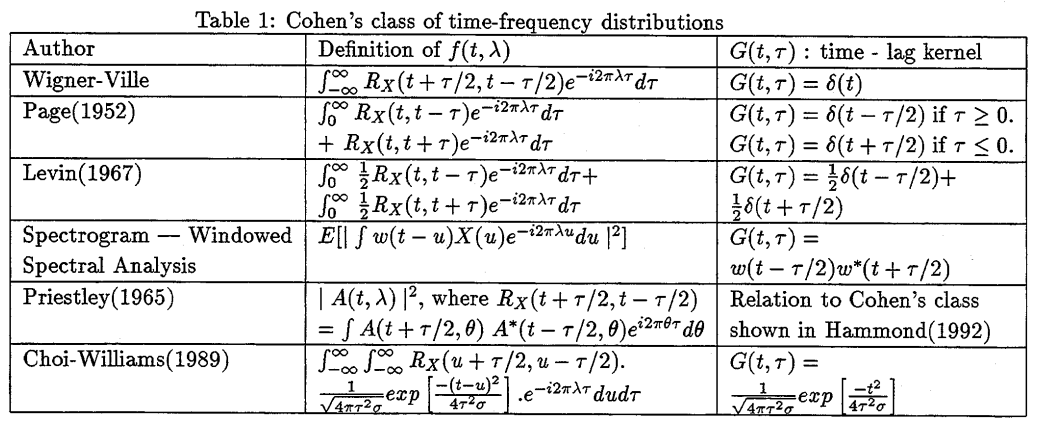
\includegraphics[width=0.9\textwidth]{tabla.png} 
\end{figure}

%Dos identidades muy importantes para estimar el espectro son la \textit{equivalencia} entre
%el espectro y la funci\'on de autocorrelaci\'on

%\begin{equation*}
%f(\omega ) = \int R_X(\tau ) e^{-i 2\pi \omega t} d\tau
%\end{equation*}
%
%Donde funci\'on de autocorrelaci\'on se ha definido como
%
%\begin{equation*}
%R_X(\tau) = E\left[ X(t) X(t+\tau) \right] = \int_0^{\infty} X(t)X(t+\tau) dt
%\end{equation*}
%
%[la demostracion es corta, batsa con reescribir una composicion de integrales como convolucion,
%la incluire mas tarde]
%
%Por otro lado, se tiene la Identidad de Parseval
%
%\begin{equation*}
%\int X^{2}(t) dt = \int f(\omega) d\omega
%\end{equation*}

%[esta demostracion se basa en la convergencia dominada del modulo de la integral de $X^{2}$ por
%la integral del modulo (...), la incluire mas tarde]

%%%%%%%%%%%%%%%%%%%%%%%%%%%%%%%%%%%%%%%%%%%%%%%%%%%%%%%%%%%%%%%%%%%%%%%%%%%%%%%%%%%%%%%%%%%%%%%%%%%

\subsection{Test Priestley-Subba Rao (PSR)}

%(seccion en proceso de re-redaccion)

A muy grosso modo, el test PSR estima localmente  el espectro evolutivo
 y revisa si estad\'isticamente
cambia en el tiempo.

Para ello, usa un estimador para la funci\'on de densidad espectral
que es aproximadamente (asint\'oticamente) insesgado y cuya varianza est\'a
determinada aproximadamente. La estimaci\'on se lleva a cabo en puntos en el tiempo y
la frecuencia tales que en conjunto son aproximadamente no-correlacionados.
Se aplica logaritmo para que la varianza de todos los estimadores sea aproximadamente
la misma (el logaritmo ayuda a), amen que los errores conjuntos tengan una
distribuci\'on cercana a una multinormal con correlaci\'on cero.
Finalmente se aplica una prueba ANOVA de varianza conocida.

%%%%%%%%%%%%%%%%%%%%%%%%%%%%%%%%%%%%%%%%%%%%%%%%%%%%%%%%%%%%%%%%%%%%%%%%%%%%%%%%%%%%%%%%%%%%%%%%%%%

\subsection{El espectro evolutivo}

Consid\'erese un proceso estoc\'astico a tiempo continuo $\{X(t)\}$, tal que
$E[X(t)]=0$ y $E\left[ X^{2}(t)\right] < \infty$ para todo $t$. Es decir que su media es constante
y sus segundos momentos est\'an bien definidos, aunque 
estos \'ultimos pueden cambiar con el tiempo.

Por el momento se supondr\'a que acepta una representaci\'on de la forma

\begin{equation*}
X(t) = \int_{-\pi}^{\pi} A(t ; \omega) e^{i\omega t} \, d Z(\omega)
\end{equation*}

Con $\{ Z(\omega) \}$ una familia de procesos ortogonales\footnote{De nuevo, esto implica que
$\Cov{dZ(\omega_1,dZ(\omega_2))} = \delta(\omega_1,\omega_1) d\omega$, una condici\'on m\'as
d\'ebil que la independencia} tales que

\begin{itemize}
\item $E \left[\abso{ dZ(\omega)}^{2} \right] = d\omega$
\item Para cada $t$ el m\'aximo de $A(t;\cdot)$ se encuentra en 0
\end{itemize}

Esta representaci\'on es an\'aloga a la representaci\'on de Cram\'er para un proceso
estacionario, salvo que se permite que la funci\'on $A$ cambie con el tiempo.
Siguiendo la analog\'ia, se define 
el \textbf{espectro evolutivo} de $\{X(t)\}$, con respecto a la la familia
$\mathcal{F} = \{ e^{i\omega t} A(t; \omega) \}$
 como
 
\begin{equation*}
d F(\omega;t) = \lvert A(t;\omega) \lvert^{2} d\omega
\end{equation*}

Ahora bien, si se supone que $\{X(t)\}$ es estoc\'asticametne diferenciable, entonces
se puede definir una \textbf{funci\'on de densidad espectral}

\begin{equation*}
f(t;\omega) = \lvert A(t;\omega) \lvert^{2}
\end{equation*}

Cabe destaca que si la funci\'on $A(t;\omega)$ fuera constante con respecto a $t$, se obtendr\'ia
un proceso estacionario de orden dos tal cual fue descrito en la secci\'on anterior.

%%%%%%%%%%%%%%%%%%%%%%%%%%%%%%%%%%%%%%%%%%%%%%%%%%%%%%%%%%%%%%%%%%%%%%%%%%%%%%%%%%%%%%%%%%%%%%%%%%%

\subsection{El estimador de doble ventana}

Esta t\'ecnica fue presentada por Priestley en 1965. Muy a grosso modo, es un estimador de la
funci\'on de densidad espectral con ciertas propiedades y que parte de la idea que un proceso
no-estacionario puede verse localmente como un proceso lineal generalizado.

Como meta-nota, yo empec\'e a estudiar este tipo de estimadores porque es \textit{el qeu ven\'ia
con el m\'etodo} ya que el test esta implementado en R; desde un punto de vista de difusi\'on,
es una ventaja usar un m\'etodo implementado en un software gratuito y de c\'odigo abierto --y
no una mera excusa para no explorar otros m\'etodos. En todo caso, he revisado varios otros test,
pero de momento solo este ha arrojado suficientes resultados para llenar un informe.

%{Estimador de doble ventana (Priestley, 1965 \& 1966)}
Para construir el estimador se reuieren dos funciones, $g$ y $w_T$, que servir\'an como ventanas
para extraer informaci\'on local de los datos. Debido a que sus propiedades tienen una interpretaci\'on
f\'isica desde la teor\'ia de circuitos, absorben su terminolog\'ia

\textit{
nota al pie: deberia incluir una motivacion de estos nombres,
que en parte tiene relevancia en la interpretacion. Los 
Linear Invariant Systems (LIS) suponen dependencia lineal
--constante-- respecto a todos los tiempos anteriores; 
a tiempo continuo son equivalentes a una ecuacion diferencial ordinaria lineal,
y a su vez a modelos AR. Un modelo fisico para ello son los circuitos RC, que
fueron usables en radios, y para los cuales las palabras 'filtro' y 'frecuencia'
tienen una interpretacion clara. Esta terminologia de circuitos electricos tiene sentido
para mi ya que todos los modelos de neuronas y poblaciones de neuronas que he visto hasta ahora,
por ejemplo de Ermentrout (falta citar), {Clark98,Priestley81}, PARTEN de considerar
circuitos equivalentes a los componentes neuronales, lo cual me hace pensar que es buena idea
mantener esta vision conjunta.
}

Primeramente se toma una funci\'on $g(u)$ normalizada, que en conjunto a su
transformada inversa de Fourier\footnote{Esta funci\'on 
$\Gamma(u) = \int_{-\infty}^{\infty} g(u) e^{i u \omega} du$
es referida como
\textbf{frequency-response function}, nombre tiene un poco de encanto cuando
$g$ adopta ciertas formas particulares (senos y cosenos).} 
$\Gamma$ tiene las siguientes propiedades

\begin{equation*}
2\pi \int_{-\infty}^{\infty} \lvert g(u) \lvert^{2} du 
= 
\int_{-\infty}^{\infty} \lvert \Gamma(\omega) \lvert^{2} d\omega
= 1
\end{equation*}


A partir de $g$ y $\Gamma$ se define el filtro $U$ como una convoluci\'on
con las realizaciones del proceso

\begin{equation*}
U(t,\omega) = \int_{t-T}^{t} g(u) X({t-u}) e^{i \omega (t-u)} du
\end{equation*}

Un ejemplo que est\'a en el libro de Priestley es tomar funciones del tipo

\begin{equation*}
g_h(u) = 
\begin{cases}
{1 \big{/} 2\sqrt{\pi h}} & \text{ , } \abso{u} \leq h
\\
0 & \text{ , } \abso{u} > 0
\end{cases}
\end{equation*}

Su correspondiente funci\'on de respuesta de frecuencia es complicada [me falta 
escribirla]. Es referida como la \textbf{ventana de Bartlett} y
est\'a totalmente caracterizada la siguiente propiedad

\begin{equation*}
\abso{\Gamma_h(\omega)}^{2} = \frac{1}{\pi h} \left( \frac{\text{sen} (h \omega)}{\omega} \right)^{2}
\end{equation*}

Cabe mencionar que puede entenderse al par $g$ y $\Gamma$ como ventanas en el tiempo
y las frecuencias para la serie.

---

Ahora bien, se toma una segunda ventana $W_\tau$ con las siguientes
restricciones para
su funci\'on de respuesta ante frecuencia $w_\tau$

\begin{itemize}
\item $w_{\tau}(t) \geq 0$ para cualesquiera $t$, $\tau$
\item $w_{\tau}(t) \rightarrow 0$ cuando $\lvert t \lvert \rightarrow \infty$, para todo $\tau$
\item $\displaystyle \int_{-\infty}^{\infty} w_{\tau}(t) dt = 1$ para todo $\tau$
\item $\displaystyle \int_{-\infty}^{\infty} \left( w_{\tau}(t) \right)^{2} dt < \infty$ para todo $\tau$
\item Existe una constante $C$ tal que  [T est\'a relacionado con el 'tiempo 0', pero para
tiempos de muestreo grandes se puede reemplazar por $-\infty$ EXCEPTO cerca del inicio y el final dle muestreo]
$$\lim_{\tau\rightarrow\infty} \left[ \tau \int_{t-T}^{t} \lvert W_{\tau}(\lambda) \lvert^{2} d\lambda \right] = C$$
\end{itemize}

%Ahora, si se define 
%$\displaystyle W_{T'}(\lambda) = \int_{-\infty}^{\infty} e^{-i\lambda t}w_{T'}(t) dt $

[posteriormente annadire mas detalles sobre el papel que juega el par $w_\tau$, $W_\tau$]

Como ejemplo, se puede tomar la siguiente funci\'on llamada \textbf{ventana de Daniell}

\begin{equation*}
W_\tau (t) = 
\begin{cases}
{1 \big{/} \tau} & \text{ , } -\nicefrac{1}{2} \tau \leq t \leq \nicefrac{1}{2} \tau
\\
0 & \text{ , otro caso}
\end{cases}
\end{equation*}

La cual se puede demostrar [tengo en algun lado esa demostracion]

$$\lim_{\tau\rightarrow\infty} \left[ \tau \int_{t-T}^{t} \lvert W_{\tau}(\lambda) \lvert^{2} d\lambda \right] = 2\pi$$

-----

Se define el estimador para $f_t$, con $0 \leq t \leq T$
\begin{equation*}
\widehat{f_t}(\omega) = \int_{t-T}^{t} w_{T'}(u) \lvert U(t-u,\omega) \lvert^{2} du
\end{equation*}

Fue demostrado por Priestley (1965, falta citar) que 

[aqui van las expresiones para el valor esperado y la varianza de $\widehat{f_t}$, me falta
escribirlas]

Pero, bajo varios supuesto adicionales [que me falta trascribir] se puede aproximar

\begin{equation*}
E\left[ \widehat{f_t}(\omega) \right] \sim f_t(\omega)
\end{equation*}

\begin{equation*}
\Var{\widehat{f_t}(\omega)} 
\sim 
\frac{C}{\tau} \left(f_t(\omega)\right)^{2} \int_{-\infty}^{\infty} \abso{\Gamma(\theta)}^{4} d\theta
\end{equation*}

Se advierte claramente que $\widehat{f_t}$ es unnestimados aproximadamente insesgado.
Para las ventanas de Bartlett y Daniell usadas como ejemplo, se tiene

\begin{equation*}
\Var{\widehat{f_t}} 
\sim 
\frac{4h}{3\tau} \left(f_t(\omega)\right)^{2}
\end{equation*}

Cabe mencionar que hay una expresi\'on expl\'icita para la covarianza de $\widehat{f_t}$
en para diferentes puntos en el tiempo y las frecuencias. Lamentablemente,
aun me falta escribirlas, son complicadas, y se describen situaciones bajo las
cuales estas covarianzas son negligibles; cabe destacar que TODAS las condiciones 
que se usan para aproximar son b\'asicamente las mismas, y dependen de que la distancia
entre los tiempos y las frecuencias sean tan grandes como sea posible.

------------

El \'ultimo ingrediente del test PSR es una transformaci\'on logar\'itmica
para regular la varianza, y quiza para cortar los bordes de las aproxiamciones.
Se define $Y_{i,j} = \log \left( \widehat{f_{t_i}}(\omega_j) \right)$, con las siguientes propiedades

\begin{equation*}
E\left[ Y_{i,j} \right] \thicksim \log \left( f_{t_i}(\omega_j) \right)
\hspace{4em}
\text{Var}\left( {Y\left(t,\omega\right)}\right) \thicksim \sigma^{2}
\end{equation*}

Luego as\'i, puede escribirse aproximadamente que

$$Y_{i,j} = \log \left( f_{t_i}(\omega_j) \right) + \varepsilon_{i,j}$$

donde $\varepsilon_{i,j}$ va iid tales que

$
E\left[ \varepsilon_{i,j} \right] = 0
\hspace{4em}
\text{Var}\left( \varepsilon_{i,j} \right) \sigma^{2}
$

Priestley cita que con esta informaci\'on incluso se puede considerar que los $\varepsilon_{i,j}$
siguen una distribuci\'on normal cada uno; Nason (2015, falta citar) comenta que
este supuesto no tiene por que cumplirse, y que es una popsible fuente de falsos positivos
para el test. Yo he hecho pruebas de normalidad a los datos, que incluire como anexos
mas tarde.

El test PSR \textit{per se} son tres test ANOVA --en su versi\'on en la que la varianza es conocida--
sobre si los $\varepsilon_{i,j}$ son estad\'isticamente negligibles en total, sobre el tiempo y sobre
las frecuencias. Para el fin de estudiar la estacionariedad, basta con que sean estad\'iticamente
no-negligibles sobre el tiempo.

[Por supuesto que los otros dos test tienen interpretacion: la negigibilidad total da informacion
sobre las marginales, y si estas pueden ser estimadas adecuadamente usando el estimador, si se
combina con negativo para no-estacionariedad es \textbf{efectivamente positivo} para estacionariedad
y toma una forma muy particular (proceso uniformemente modulado). Si sobre las frecuencias resulta
significativo (no-negligible) da informacion sobre la 'aeatoridad total' del proceso.
De tener tiempo, lo incluire como anexo, ya que ninguna de estas caracteristicas es estudiada :( ]

Lo detalles de la implementaci\'on en R estar\'an en la secci\'on de resultados.

%%%%%%%%%%%%%%%%%%%%%%%%%%%%%%%%%%%%%%%%%%%%%%%%%%%%%%%%%%%%%%%%%%%%%%%%%%%%%%%%%%%%%%%%%%%%%%%%%%%
%%%%%%%%%%%%%%%%%%%%%%%%%%%%%%%%%%%%%%%%%%%%%%%%%%%%%%%%%%%%%%%%%%%%%%%%%%%%%%%%%%%%%%%%%%%%%%%%%%%

%%%%%%%%%%%%%%%%%%%%%%%%%%%%%%%%%%%%%%%%%%%%%%%%%%%%%%%%%%%%%%%%%%%%%%%%%%%%%%%%%%%%%%%%%%%%%%%%%%%
\chapter{(Reubicar)}

\textbf{En proceso de redacci\'on}

La idea que una serie de tiempo puede no ser estacionaria, ni a\'un en un sentido d\'ebil, 
se puede rastrear en el tiempo a los a\~nos 50’s \cite{Page52,Silverman57}. 
Sin embargo, estas interrogantes en el contexto de series electrofisiol\'ogicas --en particular 
EEG-- no se ven claramente reflejados sino hasta los años 70’s 
\cite{Kawabata73,McEwen75,Cohen77,Sugimoto78}.
Esta brecha temporal se debe, quiz\'a, a la aparici\'on de computadoras digitales de bajo costo, 
gracias a las cuales es posible analizar mayores volúmenes de datos; m\'as a\'un, la escasa 
capacidad de c\'omputo promovi\'o la hip\'otesis de que las series de tiempo 
''cortas'' son estacionarias --al menos d\'ebilmente--, un hecho que ha sido 
rebatido \cite{Melard89,Adak98,Klonowski09}.

%Recientemente rige un dogma según el cual las series biológicas son –casi definición– complejas: no lineales, no estacionarias y sin equilibrio por naturaleza. Una vez se ha aceptado que las señales biológicas son naturalmente complejas, este trabajo retoma una pregunta en voga: ¿Qué implicaciones tiene haber captado una señal biológica que no es compleja? En particular, se sospecha que 

%%%%%%%%%%%%%%%%%%%%%%%%%%%%%%%%%%

%Este secci\'on contiene [va a contener] un bosquejo hist\'orico sobre los supuestos que se
%han hecho sobre la estacionariedad y otras series fisiol\'ogicas. Y es que en el resumen del
%congreso se incluyo la frase 
%
%\begin{quotation}
%Usualmente se asume que las series fisiol\'ogicas son complejas:
%no-estacionarias, no-lineales y no en equilibrio por naturaleza. Sin embargo, estas propiedades
%no se suelen probar formalmente.
%\end{quotation}

Debido a que mi trabajo pretende tomar una posici\'on opesta en alg\'un momento, en alg\'un grado,
ser\'ia incompatible que yo \textbf{simplemente suponga} que esa posici\'on es verdadera.
[Me he dado a la tarea de investigar un poco sobre el papel hist\'rico que han jugado las
hip\'otesis de regularidad en las series electrofisiol\'ogicas.]

Esta secci\'on debiera partir de los comentarios expresados 
en 'Everything you wanted to ask about EEG (..)'
(Klonowski, 2009) sobre c\'omo el concepto de ondas se acu\~na en el estudio de EEG, especilmente
de c\'omo se entienden las frecuencias en este contexto --visi\'on que es reforzada al citar
el manual de la IAAC 2007 para detectar las etaas de sue\~no.

En esta visi\'on, cabe destacar los muchos trabajos de Harmony y de Corsi-Cabrera
sobre la caracterizaci\'on y localizaci\'on de diferentes tipos de actividad cerebral 
durante diversas actividades y condiciones Adem\'as de otros autores. 
Sinceramente, son bastantes trabajos y
son la gu\'ia sobre los an\'alisis de composici\'on espectral que a\'un est\'an por hacerse.

Peor tambi\'en hay una discusi\'on sobre el balance entre los estudios espectrales contra
los avances en teor\'ia espectral: se puede citar a Cohen, quien asume que las series
cortas son b\'asicamente estacionarias. Por supuesto que cada punto en el tiempo es
t\'ecnicamente estacionario, y es completamente plausible --en el contexto de las series
electrofisiol\'ogicas-- suponer que para cada punto existe un abierto
en el tiempo tal que el subproceso definido all\'i es etsacionario para todo fin pr\'actico.
Como comenta Melard, la suposici\'on de estacionariedad para series cortas se 
consider\'o v\'alida por mucho tiempo debido a ala escasa capacidad de c\'omputo; a
modo de sintesis, Adak muestra un resultado negativo sobre la suposicion de estacionariedad
local pero muestra una prueba para detectar y medir la as\'i llamada 'estacionariedad local'.
[escribir\'e tal demostraci\'on]

En este punto, es conveniente hablar sobre los modelos ARMA como la forma mas natural de
estacionariedad a tiempo discreto, y como se usa en los modelos de estacionaeriedad 
local (citar a Adak). Se han posido generalizar estos modelos a parametros que
dependen del tiempo como los modelos ARCH (quia citar a Chatfield y a Subba Rao).

Hay una historia extensa al establecer el concepto de espectro en series no-estacionarias,
y para ello me servire de las revisiones de Loynes, Melard, Adak, Brillinger. En ella,
brillan la funcion de autocorrelacion que depende del tiempo y el que su transformada
de Fourier sea la funci\'on de densidad espectral en caso de existir. Muchas
definiciones de espectro basadas en su forma de ser calculadas.

Me gustar\'ia escribir un segundo resumen sobre el espectro de Wold-Cram\'er (el que se maneja
en el test PSR) en contraposici\'on al espectro de Wigner-Ville, el espectro de
ondeletas de Gabor y el espectro de ondeletas de Haar. Me apoyaria mucho de una discusion
hecha por Nason, de la cuakl resaltare una estimacion sobre los ordenes de tiempo de
computo para los estimadores de estos espectros.

----------------------------------------

Esta secci\'on debiera terminar nuevamente citando a Klonowski y, 
si bien no voy a usar en esta tesis, los
nuevos enfoques que consideran al EEG fundamentalmente como un sistema sujeto a ruido pero
fundamentalmente ca\'otico.

%%%%%%%%%%%%%%%%%%%%%%%%%%%%%%%%%%%%%%%%%%%%%%%%%%%%%%%%%%%%%%%%%%%%%%%%%%%%%%%%%%%%%%%%%%%%%%%%%%%

\section{EEG estacionario}

En los ochentas, antes de que las computadoras personales fueran usadas en la medicina, las
de\~nales de EEG eran registradas en una tira de papel. El registro se llevaba a cabo
en l\'ineas separadas entre s\'i por 3 cm aproximadamente, mientras que el papel se mov\'ia a 
raz\'on de 1.5, 3 o 6 cm/s seg\'un el aparato. Un m\'edico dedicado a interpetar el EEG pod\'ia
observar f\'acilmente la frecuancia de las ondas al contar el n\'umero de espigas dibujadas
en un segundo, si hab\'ia entre 2 y 30 de ellas entre dos l\'ineas verticales. De estos registros
en papel vienen los nombres cl\'asicos de las bandas, en especial las $\alpha$ y $\beta$; si las
ondas ten\'ian una frecuencia muy baja no podr\'ian distinguirse por el ojo, 
mientras que si su frecuencia era muy alta el aparato las registrar\'ia como un bloque 
indistinguible\cite{Klonowski09}.

%%%%%%%%%%%%%%%%%%%%%%%%%%%%%%%%%%%%%%%%%%%%%%%%%%%%%%%%%%%%%%%%%%%%%%%%%%%%%%%%%%%%%%%%%%%%%%%%%%%

%%%%%%%%%%%%%%%%%%%%%%%%%%%%%%%%%%%%%

%%%%%%%%%%%%%%%%%%%%%%%%%%%%%%%%%%%%%%%%%%%%%%%%%%%%%%%%%%%%%%%%%%%%%%%%%%%%%%%%%%%%%%%%%%%%%%%%%%%
%%%%%%%%%%%%%%%%%%%%%%%%%%%%%%%%%%%%%%%%%%%%%%%%%%%%%%%%%%%%%%%%%%%%%%%%%%%%%%%%%%%%%%%%%%%%%%%%%%%
\chapter{Resultados}

En cada canal que conforma el PSG (EEG, EOG y EMG), 
cada una de las \'epocas consideradas fue clasificada como 
''Posiblemente Estacionaria'' (PE) si no pudo ser rechazado la hip\'otesis de 
estacionariedad usando el test PSR ($\alpha = 0.05$), mientras que 
%el rechazo de esta misma 
%hip\'otesis es argumento ''suficiente'' para afirmar que el segmento de registro en cuenti\'on
%puede ser clasificado omo no.estacionario.
fue clasificado como ''No-estacionaria'' en caso contrario. Variar el valor cr\'itico
para la clasificaci\'on (siempre menor a 0.05) no pareci\'o generar diferencias significativas.
%La cantidad de \'epocas que no fueron para las cuales no es posible rechazar la hip\'otesis de
%estacionariedad ($\alpha=0.05$)
%clasificadas como ''Posiblemente Estacionarias'' (PE). 
La cantidad de \'epocas PE en cada individuo 
%con respecto a la cantidad total de \'epocas
durante el sue\~no MOR y no-MOR
muestra en las tablas \ref{total_gpos_mor}, \ref{total_gpos_nmor} y
\ref{total_gpos_total}; debido a que entre los sujetos hubo una gran variabilidad entre el tiempo 
que permanecieron en sue\~no MOR, se sugiri\'o comparar no el total de \'epocas PE sino
la proporci\'on --con respecto a la duraci\'on, medida en \'epocas-- de estas etapas, 
mustr\'andose estos resultados en las tablas \ref{gpos_mor}, \ref{gpos_nmor} y
\ref{gpos_total}. En estas \'ultimas tablas, se han calculado promedios y desviaciones
est\'andar muestrales entre los dos grupos que son comparados.


\begin{SidewaysFigure}
\centering
\begin{tabular}{c||ccccc||cccc||ccc}
&VCR&MJH&JAE&GHA&MFGR&CLO&RLO&RRU&JGZ&FGH&MGG&EMT \\
\hline
C3&**& &*&**& & &**&*& & & &  \\
C4&*& &***&*& & &***& & & &*&  \\
CZ&***& & & & & & & & & &***&  \\
F3&**& & &**& & &***& & & &*&** \\
F4& & & &*& & &***& & & &***&  \\
F7&*& &***&***& & & &*& & &***&*** \\
F8&**& & &**& & &*&*& & &***&  \\
FP1&***& & &*&*& & &*& & &***&  \\
FP2&***& & &*& & & & & & &***&  \\
FZ& & & &***& & &***&*& & &*&  \\
O1&*& & &***& & & & & &*& &  \\
O2& & &*&***& & &***& & & &***& \\ 
P3&*& &*&***& & &**& & & &*&  \\
P4&***& &***&*& & & & & &*&***&  \\
PZ&**& &***&*& & & &*& & &***&  \\
T3& & &**& & & &***& & & & &** \\
T4& & & &*& & &***& & & &*&  \\
T5&*& & &***& & &***& & & & &  \\
T6& & &*& & & & & & & &***&  \\
LOG&***& &***&***&**&***&**&***&*& &***&  \\
ROG&***& &***&***&*&*&***&*&*& &***&  \\
EMG& & & & & &***& &*& & & &  \\
\hline
General& & & & & &***& &*& & & & 
\end{tabular}
\caption{Diferencias significativas para la comparaci\'on entre la proporci\'on
de \'epocas PE en sue\~no MOR (fase R) y no-MOR (fases W y N).
Los asteriscos representan el pvalor con el cual se rechaza la hip\'otesis de
que las diferencias son significativas: *=0.05 , **=0.01 , ***=0.005}
\label{comparacion_mor_vs_total}
\end{SidewaysFigure}

Como un primer an\'alisis, para cada sujeto y en cada canal 
se compar\'o la proporci\'on de \'epocas PE en sue\~no MOR contra el registro completo;
el fin de ello es verificar si el sue\~no MOR --entendido como muestra no-aleatoria
del sue\~no-- tiene propiedades similares o no, y si \'esta similaridad pudiera estar
relacionada con el PDC del paciente. 
Las comparaciones se llevaron a cabo usando la prueba $\chi^{2}$ para 
proporciones\footnote{Implementada en R como la funci\'on \texttt{prop.test()}},
los resultados se muestran en la tabla \ref{comparacion_mor_vs_total}.
Se encontr\'o que no hay una relaci\'on clara entre el estado de salud del sujeto y
la aparici\'on de diferencias significativas entre estas proporciones, se hallaron
consistentemente diferencias en los canales LOG y ROG --que pueden explicarse como la actividad
ocular caracter\'istica del sue\~no MOR.
%; en la secci\'on
%de discusi\'on se mencionan algunos datos que se ''recuperaron'' de este an\'alisis.


Posteriormente se procedi\'o a comparar, por cada canal, si la proporci\'on de \'epocas PE
presenta diferencias significativas entre los grupos. Esta comparaci\'on se realiz\'o tomando
en cuenta las \'epocas de sue\~no MOR, de sue\~no no-MOR, y el registro completo 
--ver, respectivamente, tablas \ref{gpos_mor}, \ref{gpos_nmor}, \ref{gpos_total}.
Para una mejor visualizaci\'on de estos, se han graficado
% que representan
%las proporciones respectivas de cada sujeto --para ambos grupos.
en la figura \ref{comparacion_graf}
los datos de las tablas \ref{gpos_mor}, \ref{gpos_nmor} y
\ref{gpos_total}.

\begin{figure}
\centering
\subfloat[Comparaci\'on entre \'epocas MOR (fase R)]{
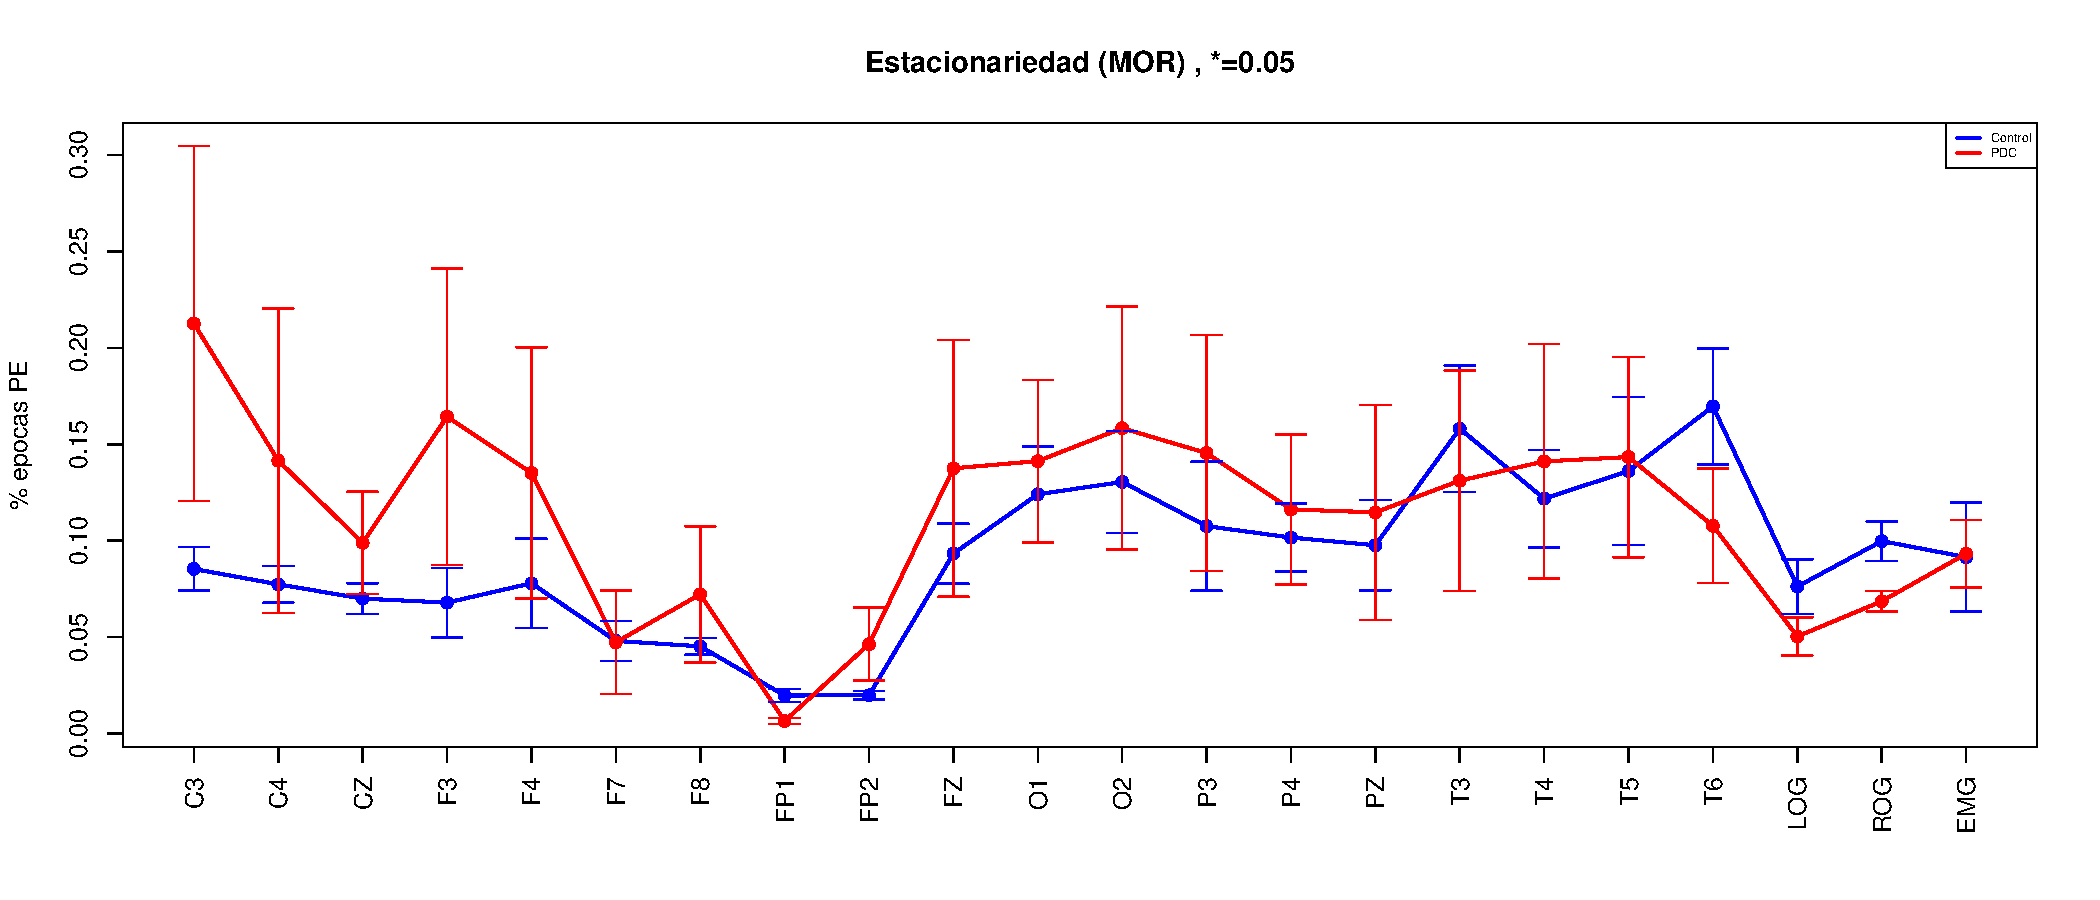
\includegraphics[width=0.95\linewidth]
{./new170424/Comparacion_gpos_MOR.pdf} 
}\\
\subfloat[Comparaci\'on entre \'epocas no-MOR (fases W y N)]{
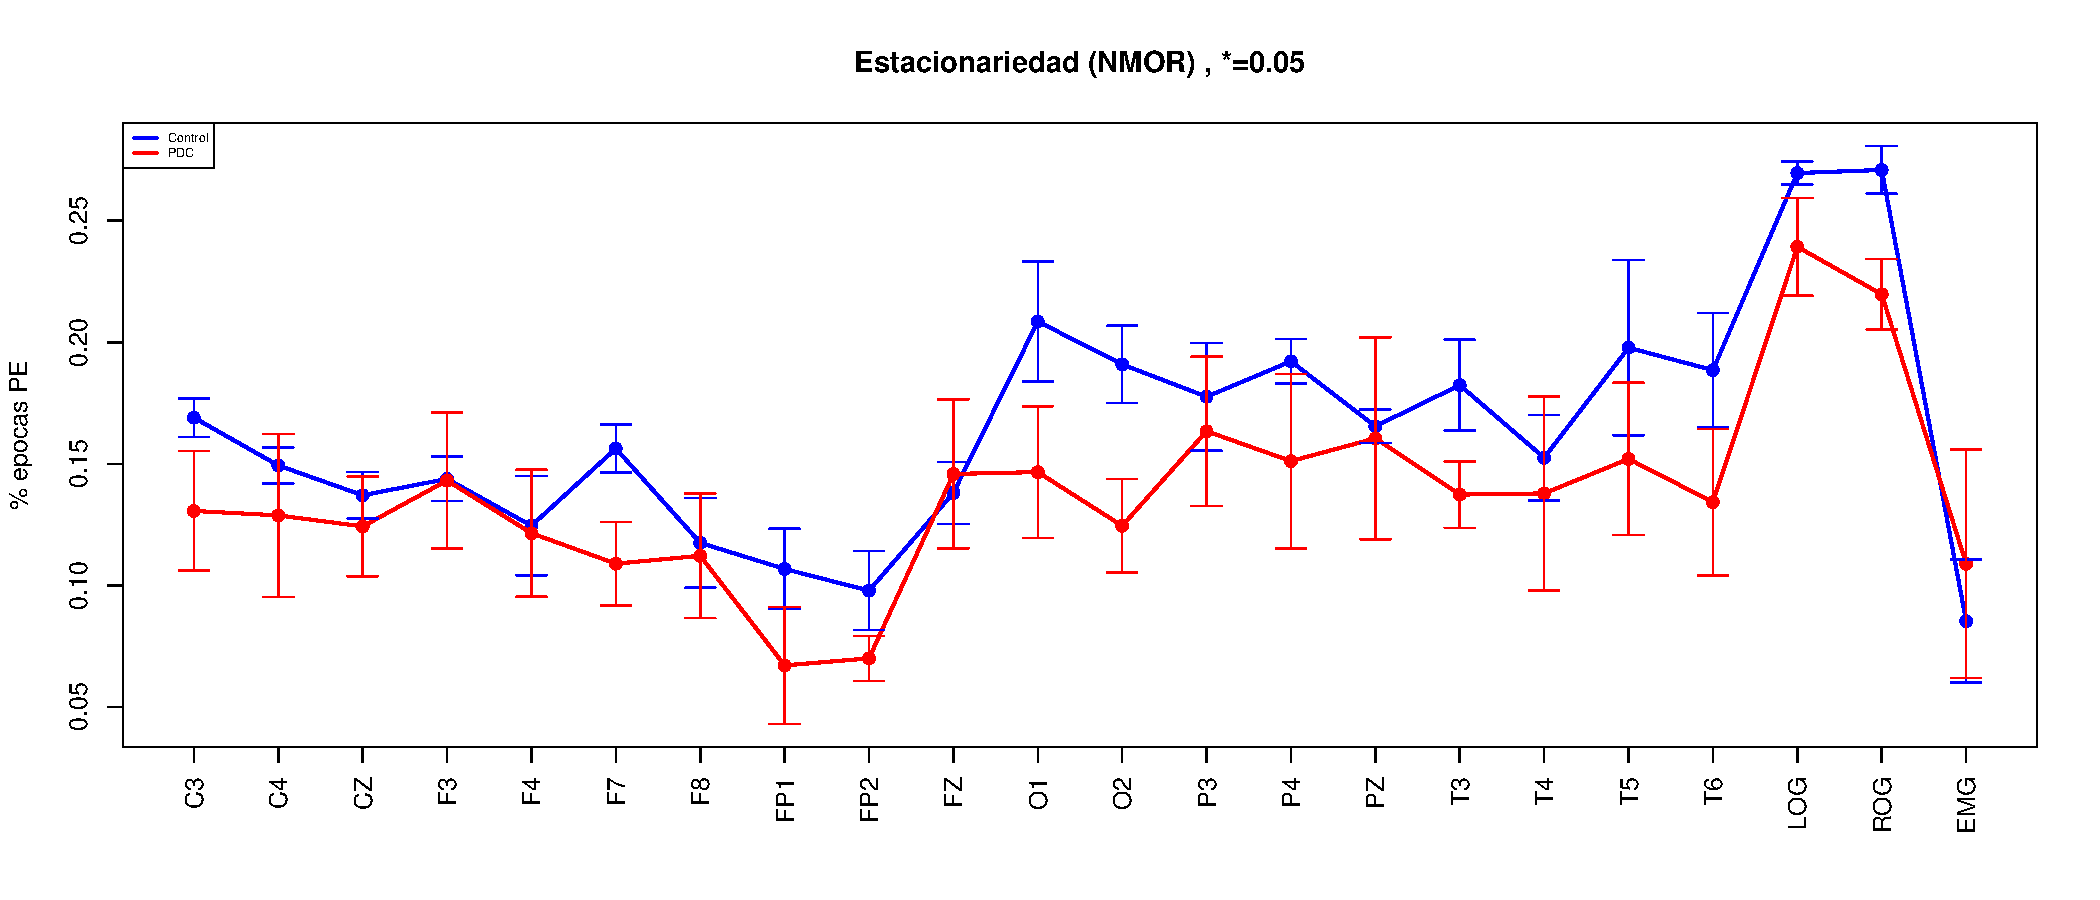
\includegraphics[width=0.95\linewidth]
{./new170424/Comparacion_gpos_NMOR.pdf} 
}\\
%\subfloat[Comparaci\'on entre el total de \'epocas registradas]{
%\includegraphics[width=0.95\linewidth]
%{./muypreeliminar170408/Comparacion_gpos_TOT.png} 
%}\\
\caption{Comparaci\'on sobre las proporciones de \'epocas PE entre los grupos, para diferentes
etapas de sue\~no. Se han graficado las proporciones de PE en todos los sujetos de ambos grupos,
as\'i como sus respectivos promedios, para cada etapa de sue\~no.}
\label{comparacion_graf}
\end{figure}

La comparaci\'on per se se llev\'o a cabo usando la prueba %no param\'etrica
%$t$ de Student y 
$U$ de Mann-Whitney\footnote{Implementada en R como la funci\'on \texttt{wilcox.test()}}.
%El primer test arroja diferencias significativas para los canales LOG, ROG y EMG, mientras que
%el segundo indica que no hay diferencias significativas. 
No se encontraron diferencias significativas para ninguno de los canales.

%Debido a que los canales
%donde se hallaron diferencias significativas no corresponden a registros de actividad
%cerebral, se considera que \textbf{esta caracter\'istica no proporciona evidencias
%suficientes sobre diferencias significativas entre adultos mayores con y sin PDC diagnosticado}.
%Este resultado es clave en el desarrollo de este trabajo.

Una tercera prueba efectuada sobre los datos fue una comparaci\'on para la proporci\'on de \'epocas
PE en cada canal, para revisar diferencias grupales entre sue\~no MOR y NMOR.
Esta prueba tiene una interpretaci\'on m\'as bien complicada, aunque su motivaci\'on es clara:
una vez hecha la comparaci\'on individial de las proporciones de PE al 
''transitar'' los sujetos entre etapas de sue\~no, y viendo que 
no hay diferencias claras entre grupos, cabe preguntarse si conviene considerar a los grupos 
como unidades.
Se encuentra que hay diferencias significativas ($\alpha<.1$) para el grupo normal
en los canales C3, C4, F7, F8, FP1, FP2, O2, P4, LOG, ROG; en el grupo PDC no se encontr\'o
ninguna diferencia.
Las diferencias encontradas pueden ser relevantes fisiol\'ogicamente, ya que 
abarcan gran parte de los l\'obulos frontal y parietal, y una regi\'on occipital-parietal derecha.
Se resta importancia a las diferencias halladas en LOG y ROG, ya que en el grupo PDC puede
aceptarse esta diferencia ''con no mucha probabilidad'' ($\alpha<.15$) y porque se esperaba
esta diferencia t\'ipica del sue\~no MOR

\begin{figure}
\centering
\subfloat[Comparaci\'on para el grupo control]{
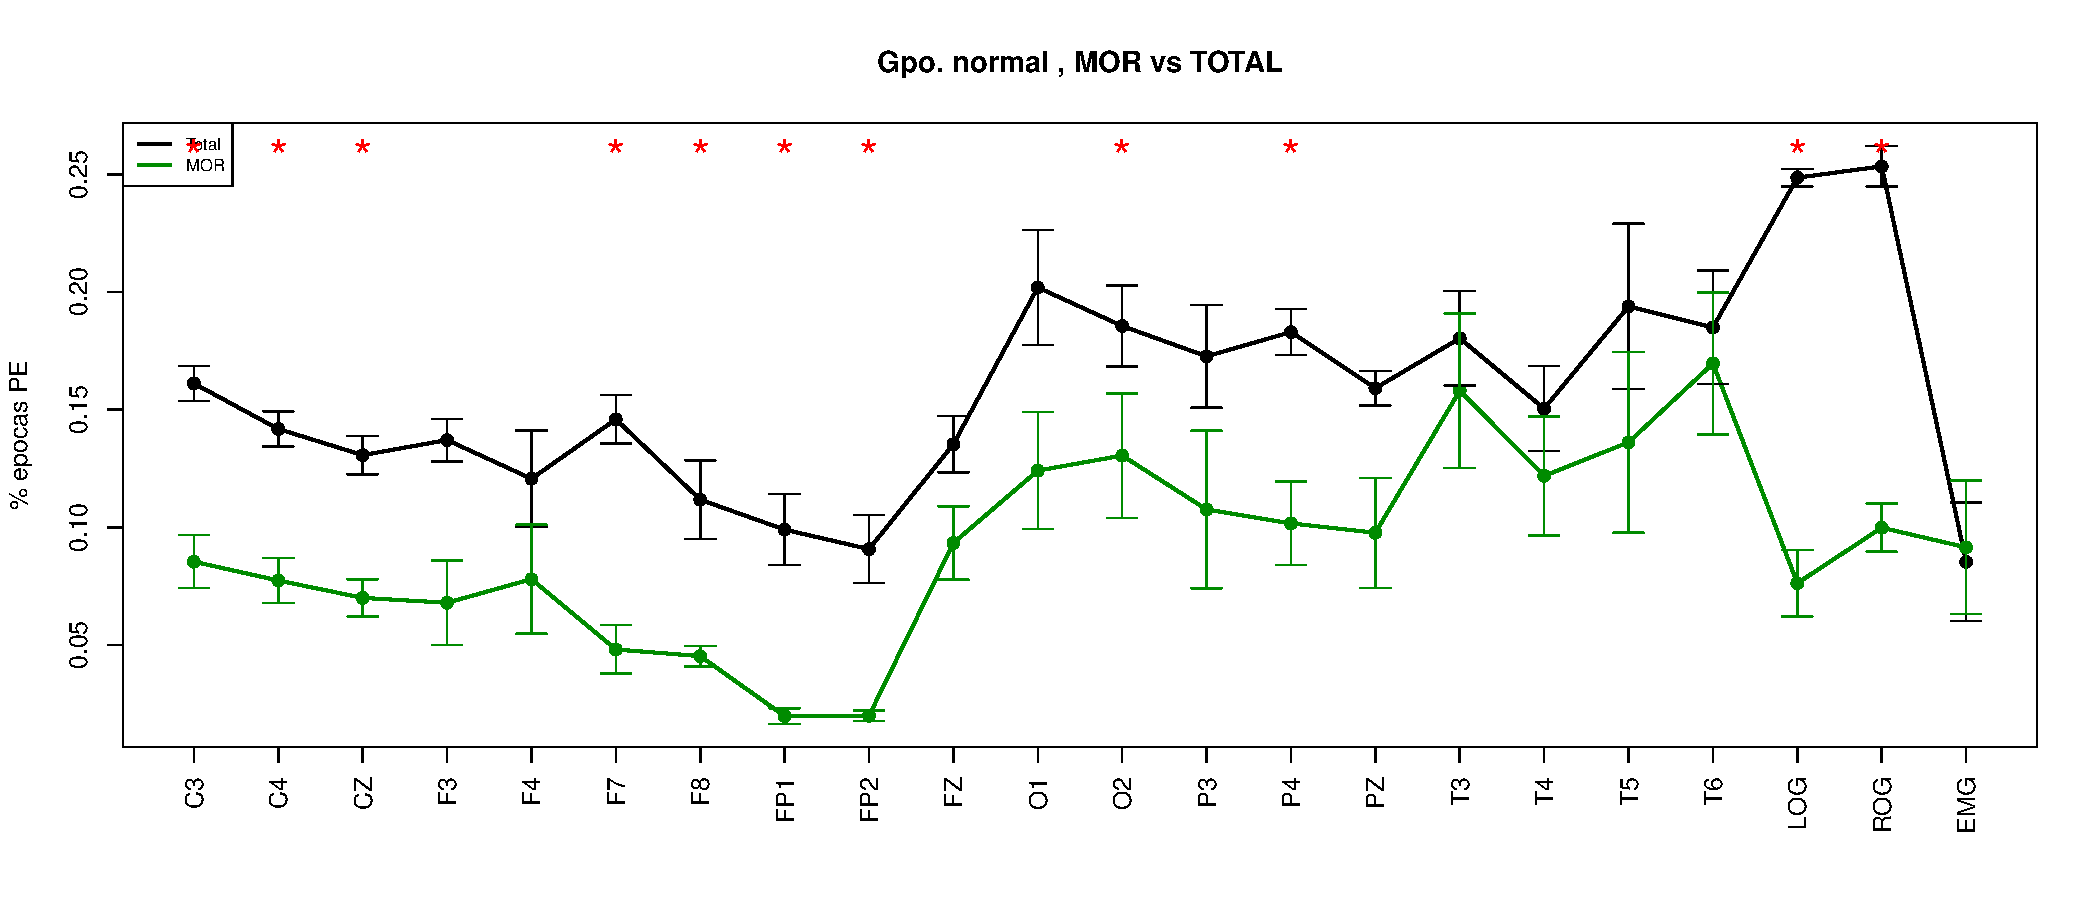
\includegraphics[width=0.95\linewidth]
{./new170424/comp_etapas_gpos_NORMALMOR_vs_TOTAL.pdf} 
}\\
\subfloat[Comparaci\'on para el grupo PDC]{
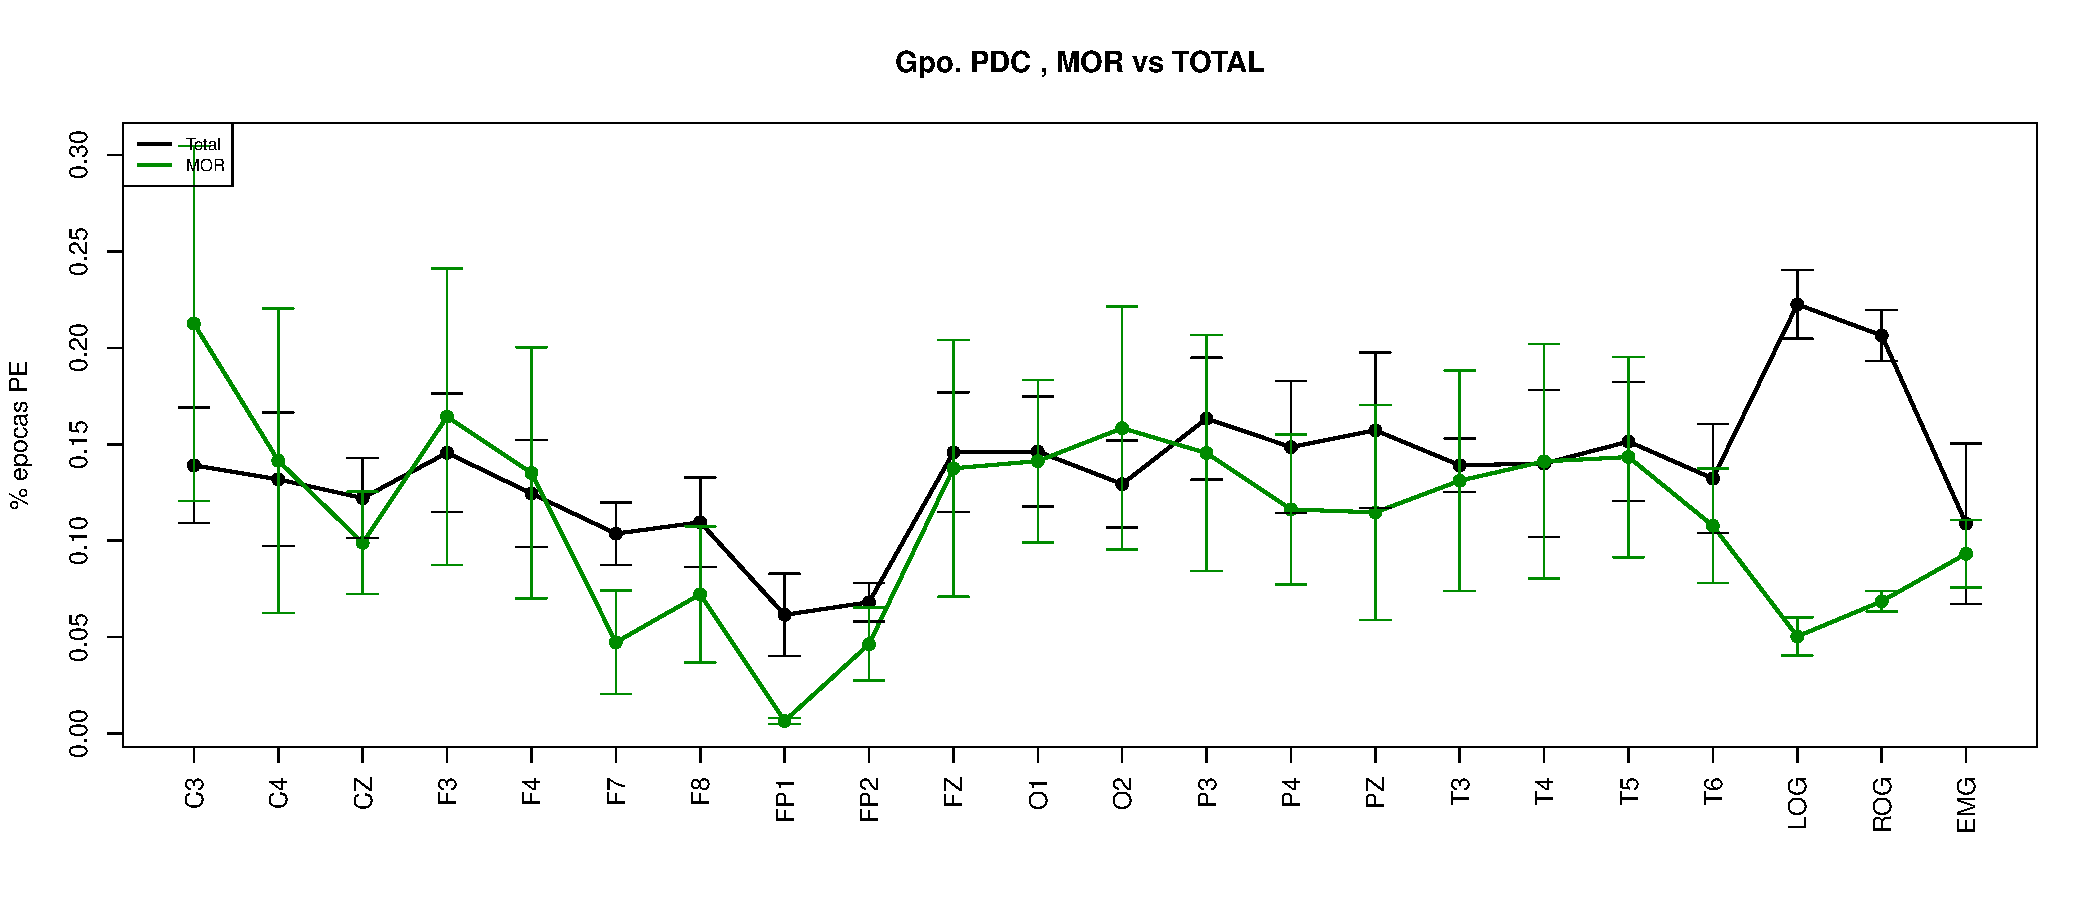
\includegraphics[width=0.95\linewidth]
{./new170424/comp_etapas_gpos_PDCMOR_vs_TOTAL.pdf} 
}\\
\subfloat[Comparaci\'on de los p-valores para aceptar diferencias]{
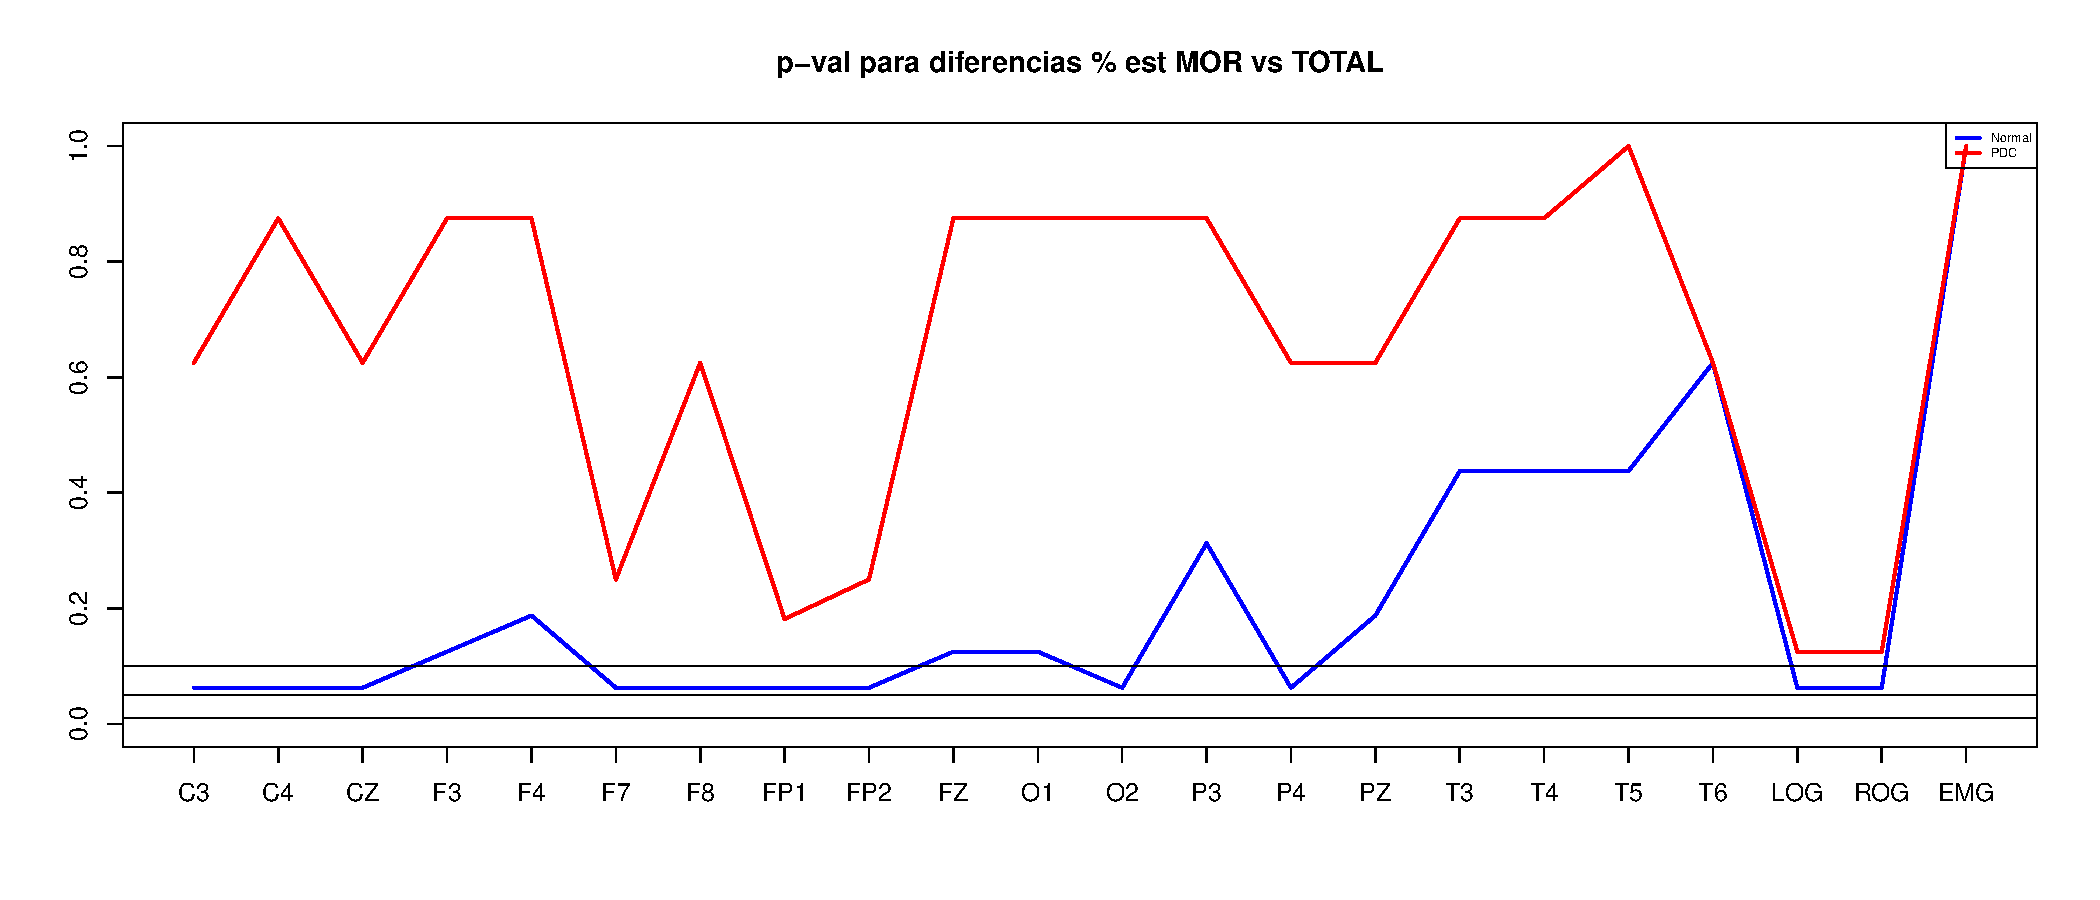
\includegraphics[width=0.95\linewidth]
{./new170424/Comparacion_pvals_gpos_MOR_vs_TOTAL.pdf} 
}\\
\caption{Comparaci\'on sobre las proporciones de \'epocas PE entre las etapas de sue\~no, 
para ambos grupos por separado. 
Se han graficado las proporciones de PE en todos los sujetos de cada grupo,
para todo el sue\~no y la etapa MOR.}
\label{comparacion_verde}
\end{figure}

\begin{figure}
\centering
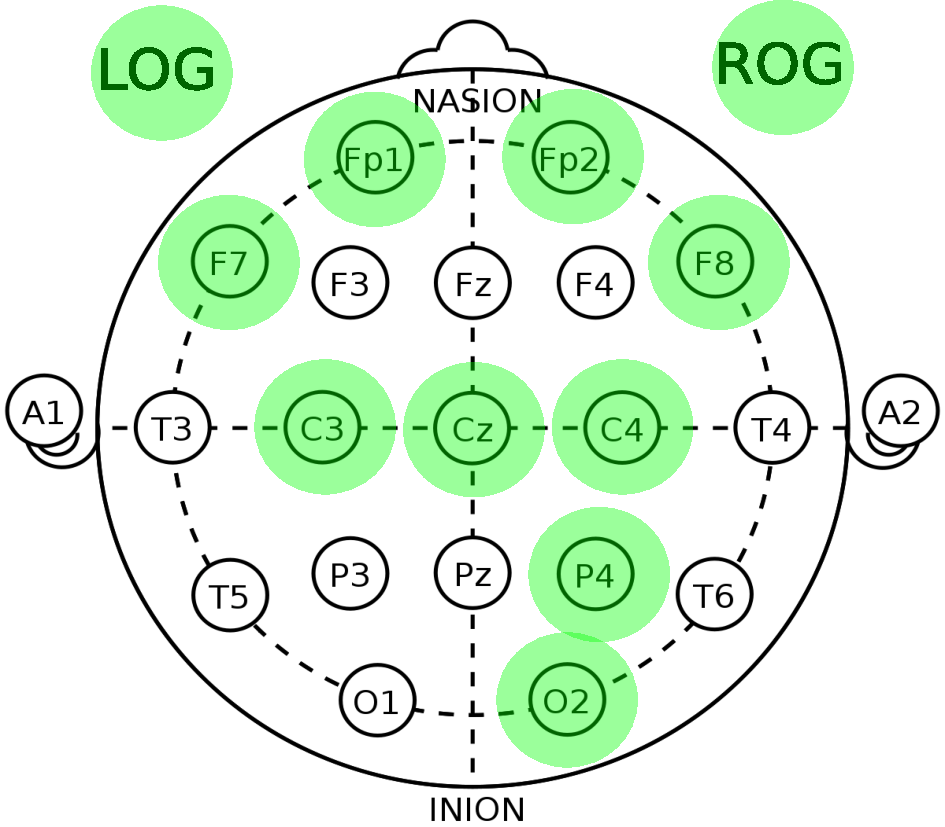
\includegraphics[width=0.65\linewidth]
{cabecita.pdf} 
\caption{Representaci\'on esquem\'atica de los sitios donde se encontraron diferencias significaticas}
\label{cabecita}
\end{figure}


Un \'ultimo an\'alisis que ser\'a reportado, es 
respecto a
una forma particular en que se han graficado los
datos obtenidos y que parece contener informaci\'on relevante.
Para esta disposici\'on gr\'afica, se colocaron en l\'inea horizontal 
''cuadros'' blanco y negros por cada
\'epoca analizada seg\'un haya sido clasificada usando el test PSR 
(blanco para PE, negro para no-estacionario)
Puede verse en la figura \ref{ejemplo_graf} un ejemplo de esta disposici\'on gr\'afica, mientras
que el resto de estos gr\'aficos se incluye como anexo.

\begin{figure}
\includegraphics[width=\textwidth]%{MJNNVIGILOS_127_mor127_tot1032_esttotal.pdf} 
{./g170413/MJNNVIGILOS_est.png}
\caption{Disposici\'on gr\'afica para los resultados del test PSR en el sujeto MJH., 
%para 1032 \'epocas de sue\~no y 22 canales. 
En el eje horizontal se muestra el tiempo desde el inicio de registro, en el eje vertical se 
muestra el nombre del canal. 
Se han resaltado con color verde las \'epocas clasificadas como de 
sue\~no MOR.
%, que son 127.
%Para este gr\'afico las \'epocas PE se clasificaron si la hip\'otesis de estacionaeriedad
%se pod\'ia rechazar la hip\'otesis de estacionariedad con en p-valor de 0.05
%seg\'un el test PSR.
}
\label{ejemplo_graf}
\end{figure}

Una debilidad 
a considerar sobre estos gr\'aficos
%importante de los gr\'aficos as\'i obtenidos 
es que, si bien hay patrones 
visuales en el tiempo,
deben ser definidos formalmente y cuantizados antes de poder ser
estudiados de manera efectiva; esta tarea ha sido poco fruct\'ifera 
y no ha aportado datos relevantes en cuanto a los objetivos planteados en un principio,
de modo que se ha exclu\'ido del cuepro principal de este trabajo.
%
% \'estos no se pueden cuantificar de una manera obvia y se dificulta la
%comparaci\'on entre sujetos, raz\'on por la cual se omiti\'o del cuerpo principal del trabajo. 
%%Se han inclu\'ido estos resultados porque sus caracter\'isticas 
%%sugieren una posible utilizaci\'on para otros fines --en alg\'un trabajo futuro.

Al ''calcular'' estos gr\'aficos para cada sujeto,
%Dentro de un mismo sujeto, 
aparecen diferencias cualitativas visibles
entre el sue\~no MOR y el resto del sue\~no nocturno; en la figura
\ref{patroncito} se muestra este patr\'on visual propuesto que,
%que vagamente est\'a caracterizado que, 
se observa, siempre contiene al sue\~no MOR si \'este no es fragmentado.
Se propone la siguiente caracterizaci\'on
para el patr\'on:
\begin{itemize}
\item Un ''bloque'' con muy pocas \'epocas PE, seguido por un bloque abundante en
\'epocas PE
\item Un bloque con una cantidad ''media'' de \'epocas PE en casi todos los canales,
excepto en LOG y ROG donde pr\'acticamente est\'an ausentes
\item Un bloque con muchas \'epocas PE en LOG y ROG, que interrumpe el bloque anterior
\end{itemize}
%Se observa que el segundo bloque siempre contiene al sue\~no MOR, si este no es fragmentado.
El tercer bloque, casi carente de \'epocas PE en los cnales LOG y ROG, parece contener
al sue\~no MOR si bien no es muy espec\'ifico. En un anexo se incluyen
todos los gr\'aficos obtenidos de esta forma.

\begin{figure}
\includegraphics[width=\textwidth]
%{./complementario170409/patrones_MJH.png}
{./graphs170427/zoom_MFGR.pdf}
\caption{Se han resaltado con color azul 
los patrones gr\'aficos 
cualitativos propuestos.}
\label{patroncito}
\end{figure}

Conviene mencionar que el origen de esta representaci\'on gr\'afica es un intento preeliminar de
fragmentar los an\'alsis de sue\~no MOR en grupos de \'epocas consecutivas en sue\~no MOR ya que,
en general, eesta etapa aparece fragmetnada durante el sue\~no nocturno \cite{CarrilloMora};
en otras palabras, existe una vaga motivaci\'on fisiol\'ogica para investigar estos patrones.
%La hip\'otesis de que se podr\'ian definir diferencias que involucraran la componente espacial,
%sin embargo, se vio opacada por la dificultad de definir formalmente tales diferencias a modo
%que pudieran compararse entre sujetos.
%Una sugerencia recibida consiste en seguir explorando estos patrones en el tiempo, pero quiz\'a
%no con la intenci\'on de detectar deterioro cognitivo sino como apoyo para la identificaci\'on de
%diferentes etapas de sue\~no.

Las hip\'otesis vertidas aqu\'i respecto a los patrones se mantendr\'an como comentarios
al cierre de este trabajo,
o como posible motivaci\'on para un trabajo futuro;
debido a que el hallazgo puede clasificarse como incidental, era menester mencionarlo.

%%%%%%%%%%%%%%%%%%%%%%%%%%%%%%%%%%%%%%%%%%%%%%%%%%%%%%%%%%%%%%%%%%%%%%%%%%%%%%%%%%%%%%%%%%%%%%%%%%%
%%%%%%%%%%%%%%%%%%%%%%%%%%%%%%%%%%%%%%%%%%%%%%%%%%%%%%%%%%%%%%%%%%%%%%%%%%%%%%%%%%%%%%%%%%%%%%%%%%%

%%%%%%%%%%%%%%%%%%%%%%%%%%%%%%%%%%%%%%%%%%%%%%%%%%%%%%%%%%%%%%%%%%%%%%%%%%%%%%%%%%%%%%%%%%%%%%%%%%%
%%%%%%%%%%%%%%%%%%%%%%%%%%%%%%%%%%%%%%%%%%%%%%%%%%%%%%%%%%%%%%%%%%%%%%%%%%%%%%%%%%%%%%%%%%%%%%%%%%%
\section{Discusi\'on}

Como se mencion\'o en la secci\'on de hip\'otesis, este trabajo pare del supuesto en que los
sujetos con PDC presentan con mayor probabilidad estacionariedad d\'ebil en sus registros de EEG.
Esta idea fue sugerida por Cohen \cite{Cohen77}, quien a su vez se refiere a trabajos anteriores
sobre regularidad estad\'stica --estacionariedad y normalidad-- sobre registros de 
EEG \cite{McEwen75,Sugimoto78,Kawabata73}. 
Si bien en estos primeros estudios se palpa la posibilidad de que los registros de EEG fueran
ruido de alg\'un tipo, esta idea se ha probado \'erronea en estudios m\'as recientes 
\cite{Klonowski09}.

Cabe entonces mencionar una segunda justificaci\'on, un poco m\'as arbitraria y personal, sobre
las hip\'otesis de este trabajo: en el trabajo de Valeria [no se como citarlo] se describen
diferencias significativas entre los registros de PSG en adultos mayores con y sin PDC,
refiri\'endose al exponente de Hurst ($H_\alpha$) estimado.
La cantidad $H_\alpha$, tambi\'en referido como el ''color'' de la se\~nal,
mide la ''fractalidad''\footnote{Este concepto no se
describir\'a en este trabajo, para m\'as informaci\'on ver el trabajo de Valeria} 
de un proceso estoc\'astico y es estimado a trav\'es del
algoritmo Detrended Fluctuation Analysis (DFA); se reporta
que el exponente $H_\alpha$ es menor para registros de PSG en adultos mayores con PSG, y que es
cercano a aqu\'el en el movimiento browniano. 
Luego entonces, cabe preguntarse sobre la naturaleza exacta de las diferencias detectadas en 
el trabajo de Valeria: ¿la se\~nal es ''menos compleja'' o 
s\'olo ''tiene otro color''?
De manera concreta, en este trabajo se ha hipotetizado sobre la primera opci\'on.

En cierto modo, se ha aportado evidencias suficientes para decir que no hay cambios significativos
en la porci\'on de tiempo durante la cual el registro de PSG se comporta de manera ''simple''
--es PE. Esto puede interpretarse como que --quiz\'a-- los mecanismos afectados durante el PDC no 
provocan que la se\~nal se vuelva m\'as simple desde el punto de vista estad\'istico

Cabe un comentario sobre c\'omo la evidencia exhibe al PSG como se\~nales no-estacionarias
por una porci\'on muy prque\~na de tiempo; luego, no es adecuado analizarla con m\'etodos que
supongan estacionariedad. M\'as a\'un este comentario aplica para individuos con y sin PDC, y
se acent\'ua m\'as en individuos con problemas adicionales.

\subsubsection{La inclusi\'on de sujetos}

%Con respecto a los sujetos con problemas adicionales, cabe mencionar el caso de FGH

Durante el trabajo se menciona constantemente a tres sujetos (FGH,MGG,EMT) que fueron considerados
pero que no son considerados dentro de las estad\'isticas; 
como se mencion\'o anteriormente,
cada uno de ellos fue exclu\'ido del
trabajo original por diversos motivos, pero dieron su consentimiento informado para la etapa
de registro de sue\~no debido a lo cual se decidi\'o analizar el efecto de su inclusi\'on dentro 
de los estad\'isticas.

El caso m\'as notorio es el sujeto FGH, quien padece de par\'alisis facial, problemas 
no especificados en la 
hipotiroides, en la columna y tiene cataratas. Seg\'un se reporta en el trabajo original,
el sujeto no inform\'o de la par\'alsis facial sino hasta despu\'es del registro de PSG, por lo
que su exlusi\'on se efectu\'o a posteriori.
Si bien la metodolog\'ia presentada aqu\'i no tiene como objetivo el diagn\'ostico
de tal padecimiento --y bajo el etendido que hay m\'etodos menos invasivos para ello--, los
registros confirman picos inusuales 


uashdflhasjkdfhlkasjdhflkajdhlkadfkasld+


\begin{comment}
\subsubsection{Otros estimadores espectrales}

Cabe mencionar que una motivaci\'on muy fuerte para utilizar el test PSR para detectar 
estacionariedad d\'ebil, tiene su origen en el objetivo informal de
''usar un m\'etodo previamente validado, f\'acil de
usar e interppretar, y que se encuentre implementado en software de f\'acil acceso''.
Este anhelo parece cumplido usando la functi\'on \texttt{stationarity} del paquete
\texttt{fractal}, en el software estad\'istico multiplataforma, gratuito y de c\'odigo abierto 
\texttt{R} --al menos en el \'ultimo punto.

Sin embargo, dado que la prueba PSR fue mostrada por primera vez en 1969 \cite{Priestley69}, es
intuitivo que debieran existir enfoques ''m\'as actuales''. En ese sentido
se puede hablar, por ejemplo, de la estimaci\'on del espectro que en este trabajo se realiz\'o a
trav\'es del estimador de doble ventana; un enfoque m\'as moderno que
cabe destacar
con mucho \'enfasis es
la familia de estimadores que satisfacen una serie depropiedades descritas por Cohen 
\cite{Cohen89} y que son referidos
como \textbf{la clase de Cohen}.
Esta clase puede ser interpretada como una ''suavizaci\'on'' del espectrograma, de forma similar al
uso de la ventana espectral; su uso parece m\'as adecuado para 
funciones 
deterministas cuyo espectro cambia en el tiempo, y se ha generalizado su uso para procesos 
d\'ebilmente estacionarios. 
El autor desconoce si existe alguna generalizaci\'on
para espectros de procesos estoc\'asticos.
%, pero se pueden exhibir trabajos donde se usan para
%calcular el espectro de realizaciones de procesos que presuponene como aleatorios [citar].
M\'as a\'un, un enfoque m\'as reciente se basa en la definici\'on de estacionariedad local

\end{comment}

\subsubsection{Otros usos para las t\'ecnicas utilizadas}

Como una etapa exploratoria de este trabajo, se dio un
%Un primer 
tratamiento cualitativo a los resultados obtenidos del test PSR
% es su
%disposici\'on gr\'afica.
grafic\'andolos de varias formas distintas; cabe destacar una de ellas que pudiera resultar
\'util pero que no hubo aportado suficiente informaci\'on clara sobre la hip\'otesis
principal de este trabajo.
%Una vez se hubo realizado el test para todas las \'epocas consideradas, se dispuso de los 
%resultados de manera gr\'afica  
%como se muestra en la figura \ref{ejemplo1}.
En esta disposici\'on gr\'afica,
se coloc\'o en l\'inea horizontal un cuadro blanco por cada
\'epoca PE (negro para \'epocas no-estacionarias);
% seg\'un el 
%el segmento en cuesti\'on halla sido clasi
%segmento referido haya sido clasificado como
%no-estacionario o posiblemente estacionario; 
posteriormente se colocaron verticalmente las
l\'ineas as\'i obtenidas.
% de todos los canales.
%Esta disposici\'on gr\'afica pretende ser consistente con las representaciones gr\'aficas
%usuales de EEG.
%, tomando en cuanta una escala m\'as amplia de tiempo gracias a que por
%cada \'epoca s\'olo se ha obtenido un dato.
Puede verse en la figura \ref{ejemplo1} un ejemplo de esta disposici\'on gr\'afica, mientras
que el resto de estos gr\'aficos se incluye como anexo.
%Los gr\'aficos as\'i obtenidos se incluyen como anexo.
%como se muestra en la figura \ref{ejemplo1}.

\begin{figure}
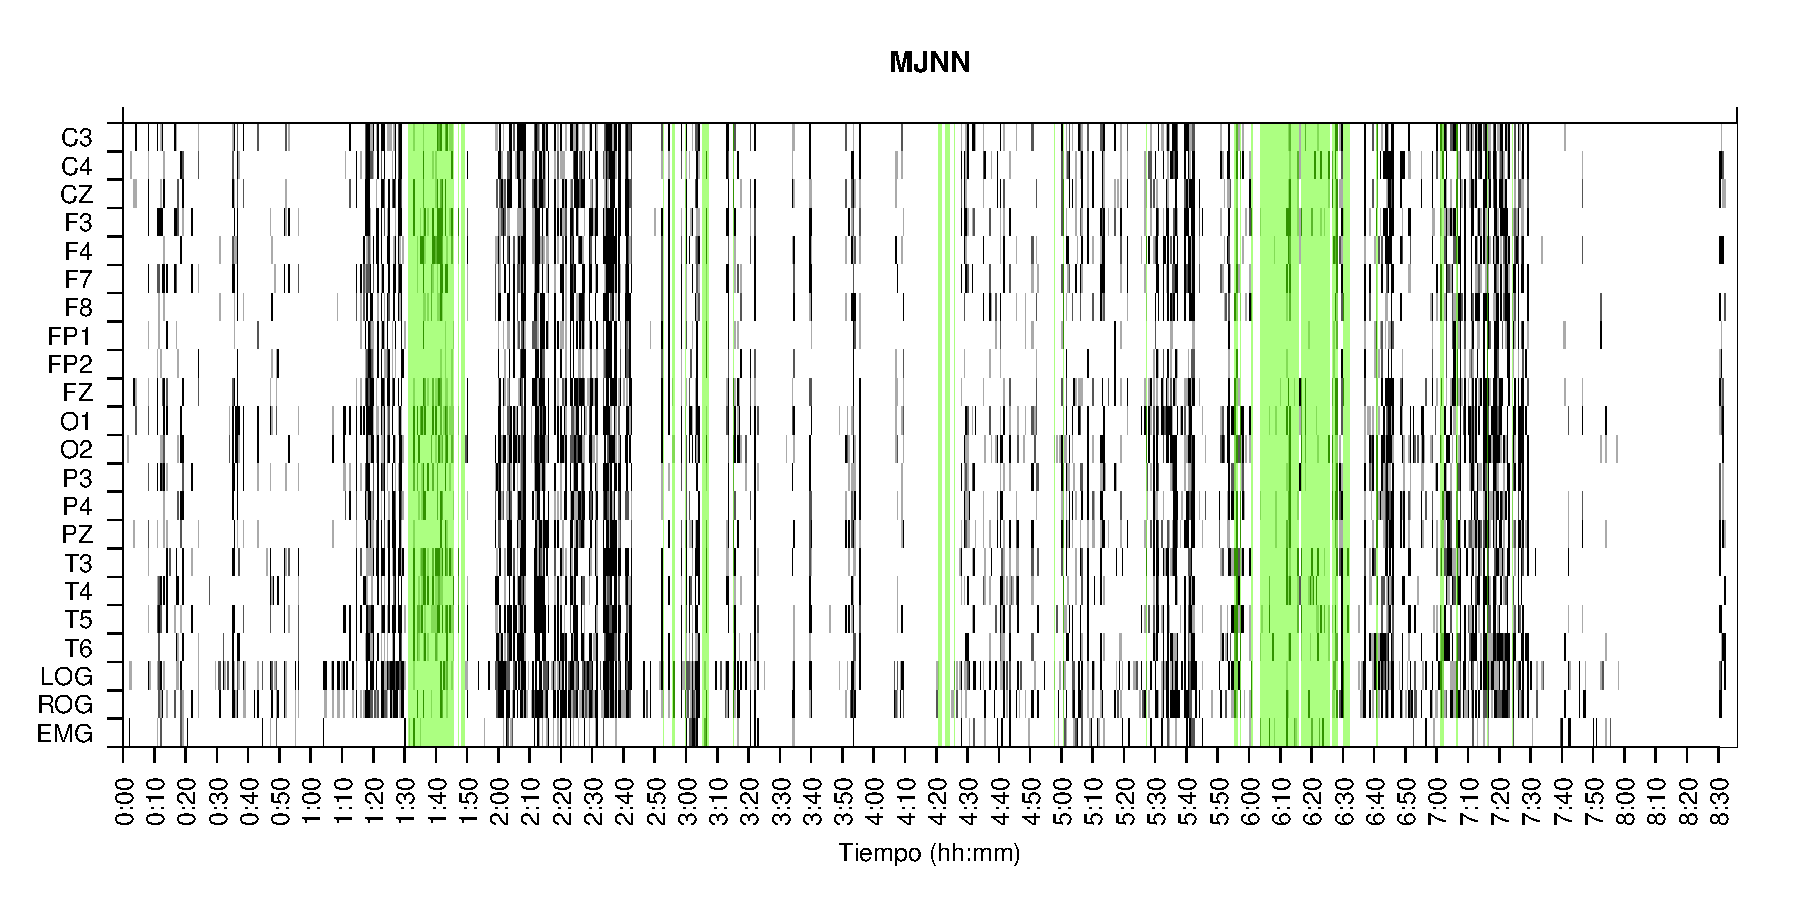
\includegraphics[width=\textwidth]{MJNNVIGILOS_127_mor127_tot1032_esttotal.pdf} 
\caption{Disposici\'on gr\'afica para los resultados del test PSR en el sujeto MJH, 
para 1032 \'epocas de sue\~no y 22 canales. 
En el eje horizontal se muestra el tiempo desde el inicio de registro, en el eje vertical se muestra al 
nombre del canal. 
Se han resaltado con color verde las \'epocas clasificadas como sue\~no MOR (ver texto), que son 127.
Para este gr\'afico se consider\'o con un p-valor cr\'itico de 0.01 para la hip\'otesis
de estacionariedad. Ver texto para m\'as detalles.}
\label{ejemplo1}
\end{figure}

Una debilidad importante de los gr\'aficos as\'i obtenidos es que, si bien muestran patrones 
claros en el tiempo, \'estos no se pueden cuantificar de una manera obvia y se dificulta la
comparaci\'on entre sujetos, raz\'on por la cual se omiti\'on del cuerpo principal del trabajo. 
%Se han inclu\'ido estos resultados porque sus caracter\'isticas 
%sugieren una posible utilizaci\'on para otros fines --en alg\'un trabajo futuro.
Sin embargo, dentro de un mismo sujeto, parecen visibles diferencias cualitativas
entre el sue\~no MOR y el resto del sue\~no nocturno.

Conviene mencionar que el origen de esta representaci\'on gr\'afica es un intento preeliminar de
fragmentar los an\'alsis de sue\~no MOR en grupos de \'epocas consecutivas en sue\~no MOR ya que,
en general, el sue\~no MOR aparece fragmetnado durante el sue\~no nocturno \cite{CarrilloMora}.
La hip\'otesis de que se podr\'ian definir diferencias que involucraran la componente espacial,
sin embargo, se vio opacada por la dificultad de definir formalmente tales diferencias a modo
que pudieran compararse entre sujetos.
Una sugerencia recibida consiste en seguir explorando estos patrones en el tiempo, pero quiz\'a
no con la intenci\'on de detectar deterioro cognitivo sino como apoyo para la identificaci\'on de
diferentes etapas de sue\~no.

%\begin{figure}
%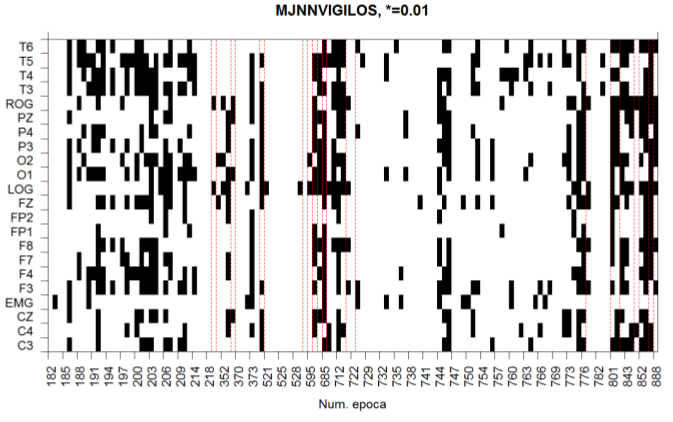
\includegraphics[width=\textwidth]{est02.png} 
%\caption{En este gráfico sólo se ilustran épocas MOR. Las líneas punteadas separan bloques continuos.
%Total de épocas: 1032 , Épocas MOR: 127}
%\label{ejemplo2}
%\end{figure}

%Me siento particularmente orgulloso
%de haber dise\~nado este tipo de gr\'aficos, ya que  organizan datos que ya se ten\'ian
%y dejan la sensaci\'on de portar nueva informaci\'on.

%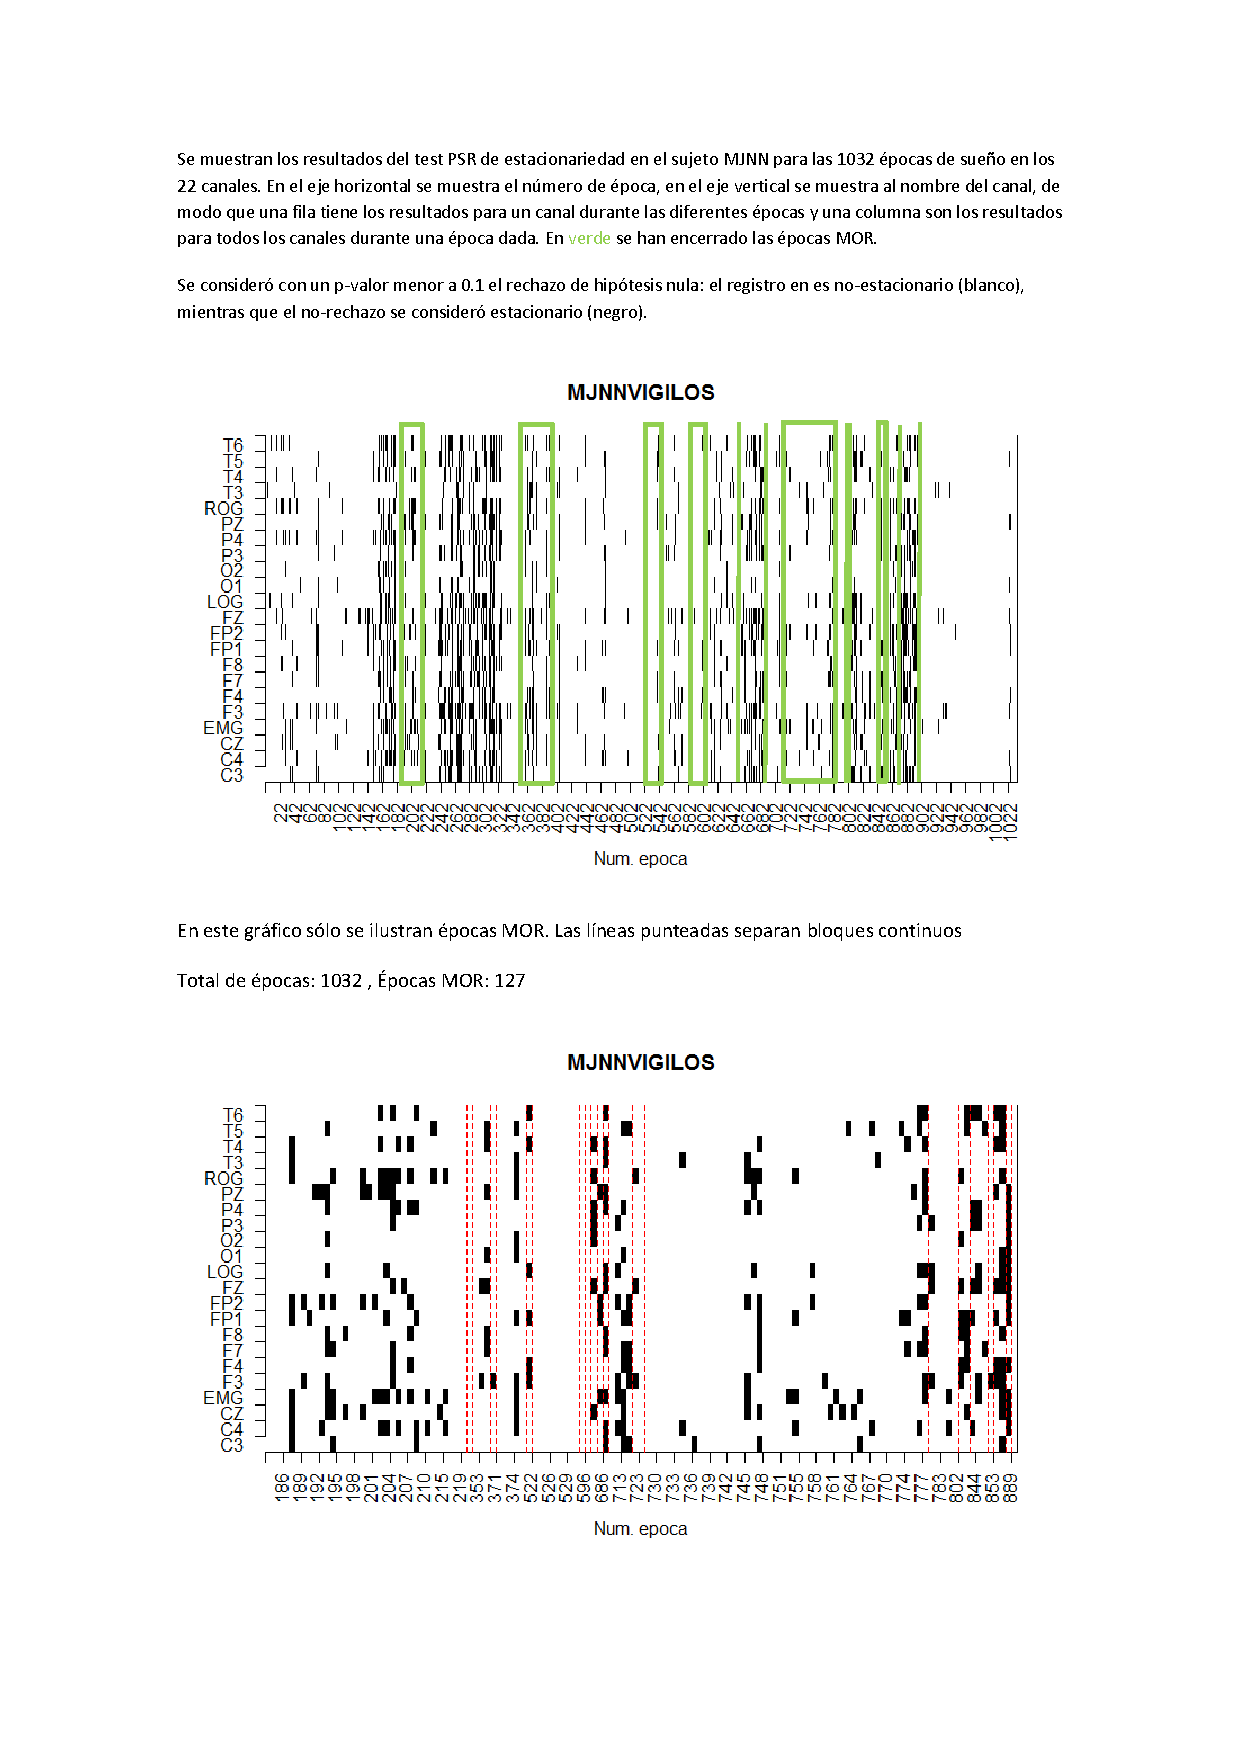
\includepdf[pages={1-},scale=.85]{reporte_de_estacionariedad_170120.pdf}
%
%\afterpage{%
%    \clearpage% Flush earlier floats (otherwise order might not be correct)
%    \thispagestyle{empty}% empty page style (?)
%    \begin{landscape}% Landscape page
%        \centering % Center table
%        \begin{figure}
%            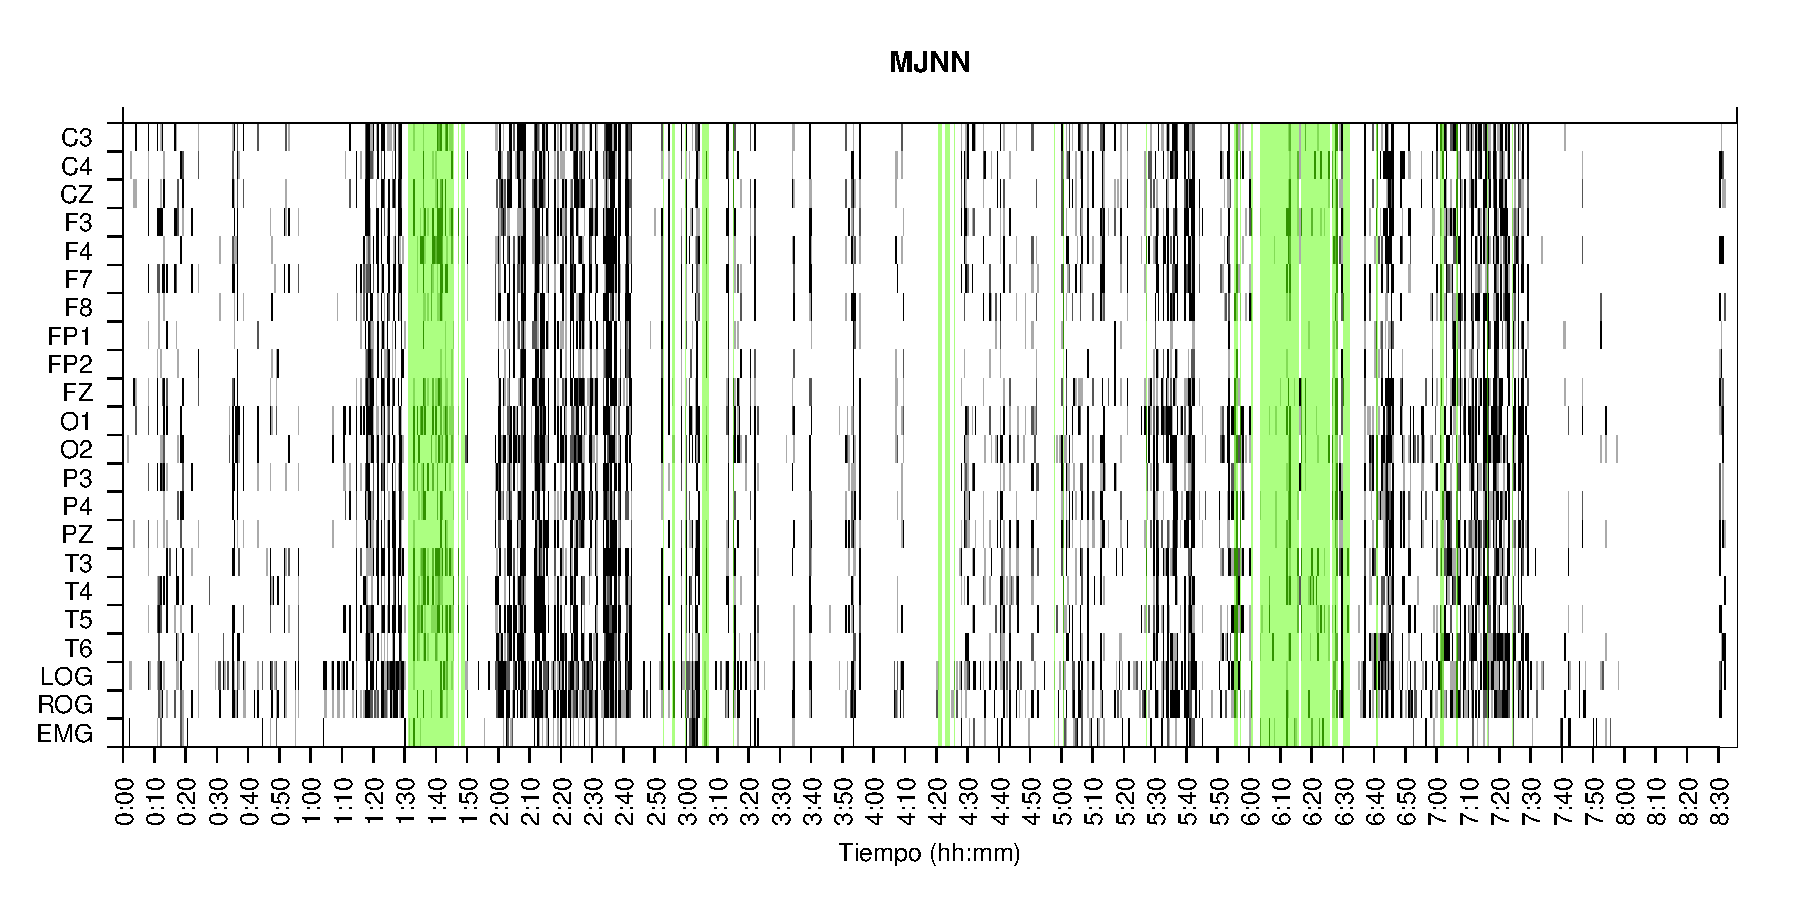
\includegraphics[width=\textwidth]{MJNNVIGILOS_127_mor127_tot1032_esttotal.pdf} 
%            \caption{Total de \'epocas: 1032, \'epocas MOR: 127}
%            %\label{ejemplo1}
%        \end{figure}
%    \end{landscape}
%    \clearpage% Flush page
%}

%%%%%%%%%%%%%%%%%%%%%%%%%%%%%%%%%%%%%%%%%%%%%%%%%%%%%%%%%%%%%%%%%%%%%%%%%%%%%%%%%%%%%%%%%%%%%%%%%%%
%%%%%%%%%%%%%%%%%%%%%%%%%%%%%%%%%%%%%%%%%%%%%%%%%%%%%%%%%%%%%%%%%%%%%%%%%%%%%%%%%%%%%%%%%%%%%%%%%%%

\section{Conclusiones}

Se aportan evidencias sobre que la presencia proporcional de estacionariedad d\'ebil en registros 
de PSG para adultos mayores, 
no presenta diferencias significativas entre sujetos con y sin PDC diagnosticado.
Luego entonces, esta caracter\'istica no es un indicador fiable 

%%%%%%%%%%%%%%%%%%%%%%%%%%%%%%%%%%%%%%%%%%%%%%%%%%%%%%%%%%%%%%%%%%%%%%%%%%%%%%%%%%%%%%%%%%%%%%%%%%%
%%%%%%%%%%%%%%%%%%%%%%%%%%%%%%%%%%%%%%%%%%%%%%%%%%%%%%%%%%%%%%%%%%%%%%%%%%%%%%%%%%%%%%%%%%%%%%%%%%%

\section{Trabajo a futuro}

Como se ha sugerido, los bloques de estacionariedad pueden tener un uso como 
caracter\'isticas auxiliares
para la detecci\'on autom\'atica de \'epocas MOR en registros de PSG: el hecho que la proporci\'on
de \'epocas PE no se vea afectada --estad\'isticamente-- por el PDC del paciente, sugiere que es
posible obtener resultados independientes de ello. Para ello cabe recordar, como se mencion\'o 
en la secci\'on de discusi\'on, que sujetos fuera del rango de los grupos considerados puede
que fallen respecto a esta conclusi\'on: hace falta m\'as indagaci\'on al respecto. 

Por otro lado, el uso de estimadores espectrales de ventana pueden explorarse de manera m\'as
puntual para detectar estacionariedad sobre componentes de frecuencia espec\'ificas, de modo
que es en principio posible separar las ondas cerebrales.

%%%%%%%%%%%%%%%%%%%%%%%%%%%%%%%%%%%%%%%%%%%%%%%%%%%%%%%%%%%%%%%%%%%%%%%%%%%%%%%%%%%%%%%%%%%%%%%%%%%
%%%%%%%%%%%%%%%%%%%%%%%%%%%%%%%%%%%%%%%%%%%%%%%%%%%%%%%%%%%%%%%%%%%%%%%%%%%%%%%%%%%%%%%%%%%%%%%%%%%

\appendix

\chapter{Resultados no re-redactados}

Estos reultados ya fueron presentados a la Dra Rosales Lagarde de ICSA, con quien se
trabajo si eran de relevancia fisiologica o no. Aun me falta redactar como texto las conclusiones
encontradas, y que tengo dispersas como notas. 

Cabe mencionar que se incluyen partes de un analisis
sobre somposicion de frecuencias sobre el que no he hablado para nada en el resto del texto,
y es que apenas y se esta trabajando en ello: he priorizado en el tiempo la redaccion
sobre  las bases
formales del test PSR, porque ya esta batsante avanzado y no habia escrito al respecto nada que fuera
suficientemente bueno. Si continuaba con esta actitud, ocurriria lo mismo con el analisis por bandas.

Aunque parece impresionante porque eleva el numero de paginas, son imagenes cuyo analisis puede 
reducirse a menos de 5 p\'aginas. Estas im\'agenes son muy importantes
porque muestran una suerte de distribuci\'ion temporal y --de manera reducida-- espacial 
de algunas caracter\'isticas de la se\~nal. 

Me siento particularmente orgulloso
de haber dise\~nado este tipo de gr\'aficos, ya que 
simlemente organizan
gr\'aficamente los datos que ya se ten\'ian de una forma
totalmente contraria a algo novedoso,
y a\'un as\'i dejan la sensaci\'on de portar nueva informaci\'on.

%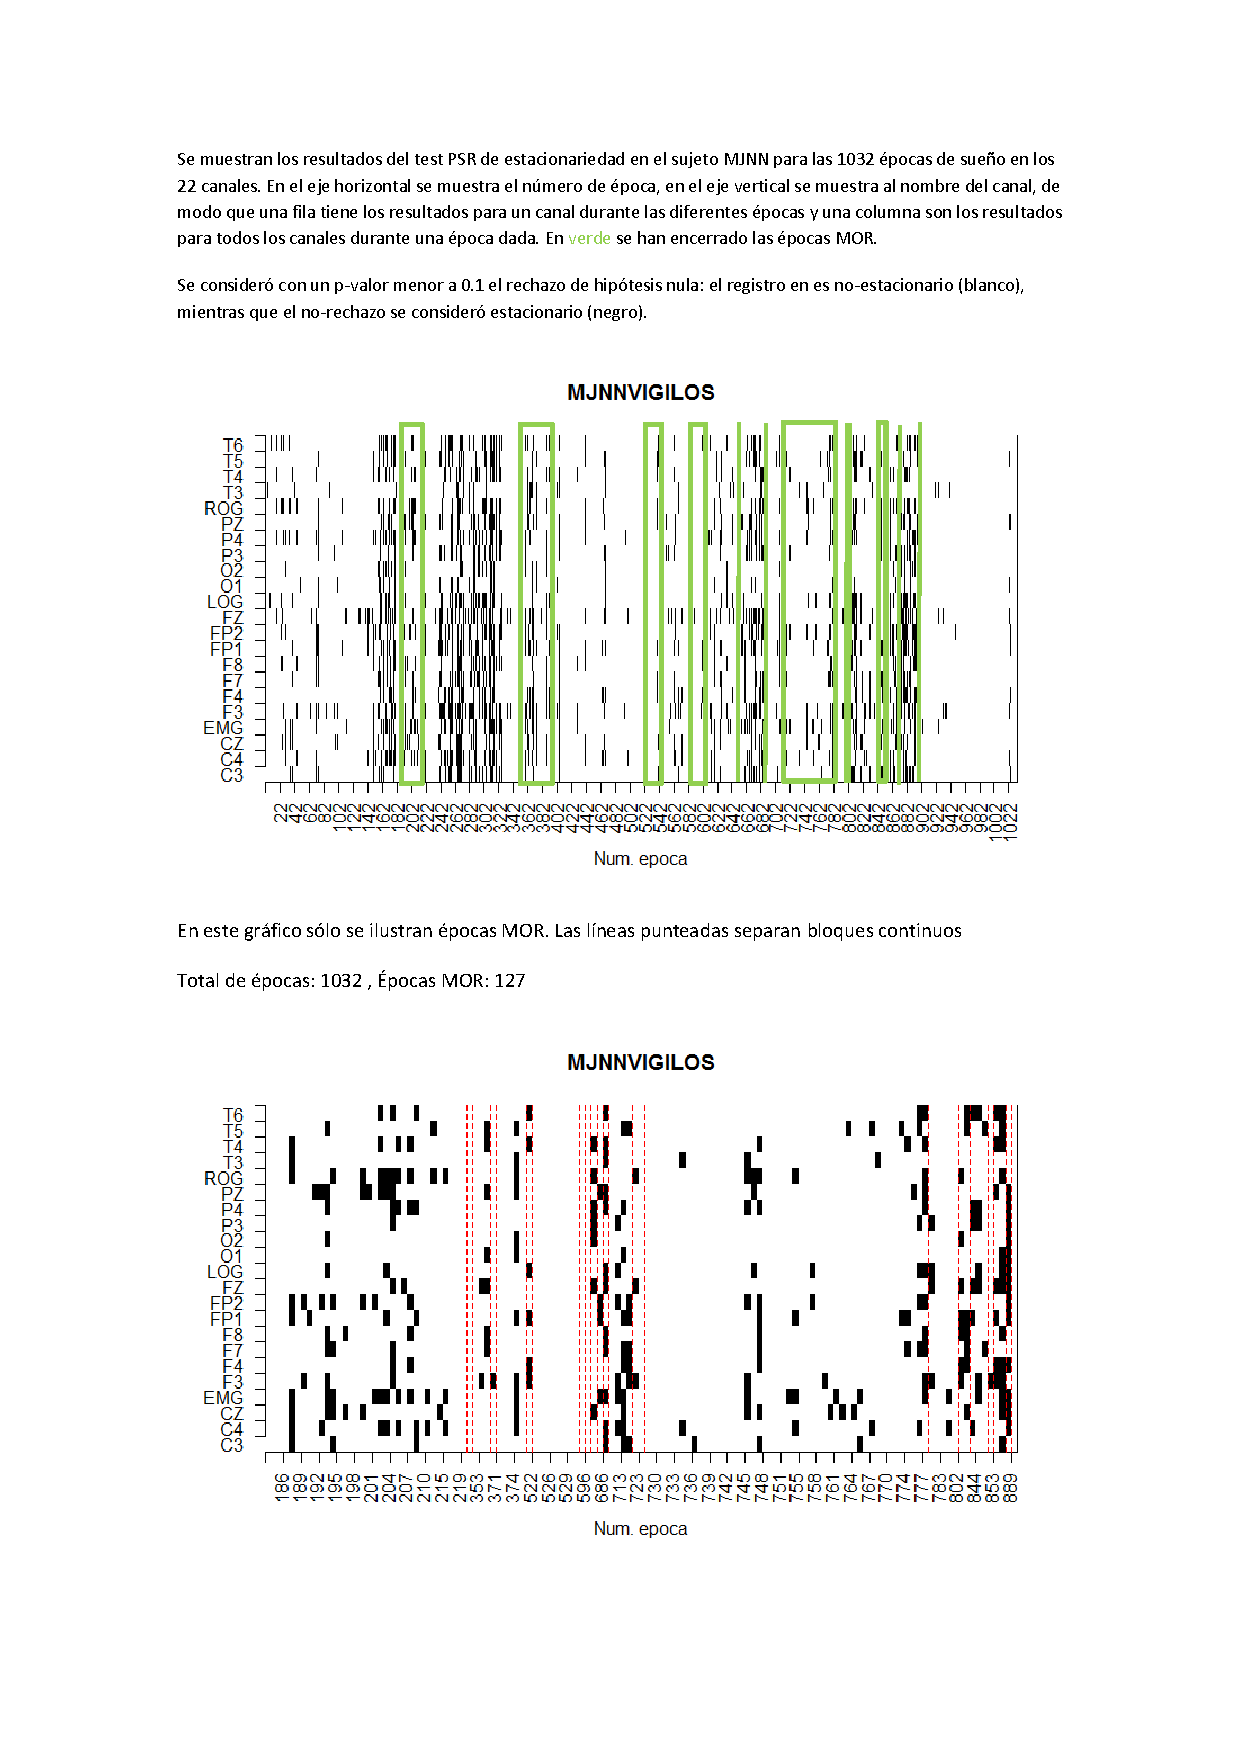
\includepdf[pages={1-},scale=.85]{reporte_de_estacionariedad_170120.pdf}

%%%%%%%%%%%%%%%%%%%%%%%%%%%%%%%%%%%%%%%%%%%%%%%%%%%%%%%%%%%%%%%%%%%%%%%%%%%%%%%%%%%%%%%%%%%%%%%%%%%
%%%%%%%%%%%%%%%%%%%%%%%%%%%%%%%%%%%%%%%%%%%%%%%%%%%%%%%%%%%%%%%%%%%%%%%%%%%%%%%%%%%%%%%%%%%%%%%%%%%

\bibliography{referencias_estacionariedad,referencias_fisiologia,referencias_otros}{}
%\bibliographystyle{apalike-es}
\bibliographystyle{plain}

%%%%%%%%%%%%%%%%%%%%%%%%%%%%%%%%%%%%%%%%%%%%%%%%%%%%%%%%%%%%%%%%%%%%%%%%%%%%%%%%%%%%%%%%%%%%%%%%%%%
%%%%%%%%%%%%%%%%%%%%%%%%%%%%%%%%%%%%%%%%%%%%%%%%%%%%%%%%%%%%%%%%%%%%%%%%%%%%%%%%%%%%%%%%%%%%%%%%%%%

\end{document}